% !TEX program = pdflatex
%=====================================================================
%  Criptografía y Seguridad — ITBA · Segunda Parte
%  Parciales resueltos (mapeo ejercicio → temas + resolución)
%  Documento maestro: preámbulo + \input de cada fragmento.
%=====================================================================
\documentclass[11pt,a4paper]{article}

\usepackage[utf8]{inputenc}
\usepackage[T1]{fontenc}
\usepackage[spanish,es-tabla,es-noshorthands]{babel}
\usepackage{lmodern}
\usepackage{microtype}

\usepackage{amsmath,amssymb,amsthm}
\usepackage{mathtools}
\usepackage{geometry}
\geometry{a4paper,margin=2.4cm,headheight=24pt}

\usepackage{xcolor}
%---- Paleta ITBA ----
\definecolor{itbaCyan}{HTML}{6EC6D9}
\definecolor{itbaCyanDark}{HTML}{2E8B9E}
\definecolor{itbaBlue}{HTML}{AEDCEA}
\definecolor{boxBlue}{HTML}{BBD4F0}
\definecolor{slideGray}{HTML}{ECECEC}
\definecolor{practGreen}{HTML}{4F8A3D}
\definecolor{practGreenL}{HTML}{E2EFD9}
\definecolor{attackRed}{HTML}{C0392B}
\definecolor{codeBg}{HTML}{F5F5F5}

\usepackage{graphicx}
\usepackage{enumitem}
\usepackage{booktabs}
\usepackage{array}
\usepackage{longtable}
\usepackage{tcolorbox}
\tcbuselibrary{skins,breakable}
\usepackage{fancyhdr}
\usepackage{titlesec}
\usepackage{listings}
\usepackage{caption}
\usepackage{pifont}
\usepackage{pdfpages}
\usepackage{tikz}
\usetikzlibrary{shapes.geometric,shapes.misc,shapes.symbols,arrows.meta,positioning,
                calc,fit,backgrounds,decorations.pathmorphing,decorations.pathreplacing,
                decorations.markings,shadows.blur,chains,matrix}
\usepackage{hyperref}
\hypersetup{colorlinks=true,linkcolor=itbaCyanDark,urlcolor=itbaCyanDark,
            citecolor=itbaCyanDark,linktoc=all,
            pdftitle={Parciales resueltos - Cripto Segunda Parte},
            pdfauthor={Criptografia y Seguridad - ITBA}}

%---- Encabezados ----
\pagestyle{fancy}
\fancyhf{}
\lhead{\small\textsc{Criptografía y Seguridad — ITBA}}
\rhead{\small Parciales resueltos · Segunda Parte}
\cfoot{\small\thepage}
\renewcommand{\headrulewidth}{0.4pt}

%---- Títulos de sección con barra de color ----
\titleformat{\section}
  {\normalfont\Large\bfseries\color{itbaCyanDark}}
  {\thesection}{0.6em}{}
  [\vspace{-0.4em}{\color{itbaCyan}\titlerule[2pt]}]
\titleformat{\subsection}
  {\normalfont\large\bfseries\color{itbaCyanDark}}
  {\thesubsection}{0.6em}{}

%---- Estilo de código ----
\lstdefinestyle{code}{
  basicstyle=\ttfamily\footnotesize, backgroundcolor=\color{codeBg},
  keywordstyle=\color{itbaCyanDark}\bfseries, commentstyle=\color{practGreen}\itshape,
  stringstyle=\color{attackRed}, breaklines=true, frame=single,
  rulecolor=\color{black!30}, showstringspaces=false, columns=fullflexible, tabsize=2,
  xleftmargin=10pt, framexleftmargin=8pt}
\lstset{style=code}

%=====================================================================
%  Entorno requerido por los fragmentos: consigna textual del parcial
%=====================================================================
\newtcolorbox{consigna}{
  breakable, enhanced, colback=slideGray, colframe=black!55, boxrule=0.6pt, arc=2pt,
  left=8pt,right=8pt,top=6pt,bottom=6pt, fonttitle=\bfseries, coltitle=white,
  title={Consigna (textual)}}

% Cajas auxiliares (por si algún fragmento las usa)
\newtcolorbox{defbox}[1]{enhanced,breakable,colback=itbaBlue!25,colframe=itbaCyanDark,
  boxrule=1pt,arc=2pt,fonttitle=\bfseries,coltitle=white,title={#1}}
\newtcolorbox{warnbox}[1]{enhanced,breakable,colback=attackRed!8,colframe=attackRed,
  boxrule=1pt,arc=2pt,fonttitle=\bfseries,coltitle=white,title={#1}}
\newtcolorbox{practbox}[1]{enhanced,breakable,colback=practGreenL,colframe=practGreen,
  boxrule=1pt,arc=2pt,fonttitle=\bfseries,coltitle=white,title={#1}}

%---- Macros de control de acceso usadas por los fragmentos ----
\newcommand{\dom}{\ensuremath{\succeq}}        % relación de dominancia
\newcommand{\Lvl}{\ensuremath{\mathrm{L}}}     % nivel de seguridad L(·)
\newcommand{\il}{\ensuremath{\mathrm{i}}}      % nivel de integridad i(·)
\providecommand{\cmark}{\ding{51}}
\providecommand{\xmark}{\ding{55}}

%=====================================================================
\begin{document}
%=====================================================================

\begin{titlepage}
\centering
\vspace*{2cm}
{\Huge\bfseries\color{itbaCyanDark} Parciales Resueltos}\\[0.4cm]
{\LARGE Criptografía y Seguridad — Segunda Parte}\\[0.3cm]
{\large Mapeo ejercicio → temas + resolución, con \emph{retrieval} sobre los informes}\\[1.2cm]
{\normalsize Instituto Tecnológico de Buenos Aires (ITBA)}
\vfill
{\footnotesize\itshape Generado a partir de los parciales en \texttt{parciales/} y los informes
(\texttt{informes-pina/}) / resúmenes (\texttt{resumenes/unidades/}), siguiendo el índice de temas.}
\end{titlepage}

\tableofcontents
\newpage

%=====================================================================
\section*{Cómo está armado}
\addcontentsline{toc}{section}{Cómo está armado}
%=====================================================================
Cada parcial es una \textbf{sección}; cada ejercicio, una \textbf{subsección} con: la
\emph{consigna textual}, los \emph{temas} que toca (referidos como ``Clase X — Tema''), \emph{qué
necesitás saber}, \emph{notas y conexiones}, y la \emph{resolución}. La prioridad de fuentes es
\textbf{informe sobre resumen}; las Clases 10/10b/11 solo tienen resumen.

\medskip
\noindent\textbf{Notas de cobertura:}
\begin{itemize}[leftmargin=1.4em,itemsep=2pt]
  \item \textbf{Parcial 2023 Q1} es en realidad de la \emph{Primera Parte} (criptografía pura):
        se transcribe y mapea, pero la mayoría de sus ejercicios queda fuera del alcance de la
        Segunda Parte (marcados con \texttt{TODO: Primera Parte}).
  \item El archivo ``Segundo Parcial 2017'' trae internamente el encabezado ``Parcial 2 -- 2015'';
        se conservó el rótulo del archivo y se dejó la observación en su sección.
  \item En los Shamir, la reconstrucción por interpolación de Lagrange no está en las fuentes del
        curso (que cubren Shamir \emph{vía entropía}); el cálculo numérico se hizo y verificó aparte.
\end{itemize}

%=====================================================================
\section*{Material fuente (enlaces)}
\addcontentsline{toc}{section}{Material fuente (enlaces)}
%=====================================================================
Los informes/resúmenes y los parciales originales están \textbf{embebidos al final} de este
documento (Apéndice). Los enlaces de abajo \textbf{saltan internamente} a la primera página de
cada uno: funcionan en \emph{cualquier} visor —incluida Vista Previa— y el archivo es un único
PDF portable. (Los PDFs sueltos también quedan en \texttt{./pdfs/} por si los querés aparte.)

\paragraph{Informes / resúmenes por clase.}
\begin{itemize}[leftmargin=1.4em,itemsep=1pt]
  \item \hyperref[src:clase6]{Clase 6 — Políticas y Control de Acceso} (informe)
  \item \hyperref[src:clase7]{Clase 7 — Autenticación} (informe)
  \item \hyperref[src:clase8]{Clase 8 — Principios de Diseño y Vulnerabilidades} (informe)
  \item \hyperref[src:clase9]{Clase 9 — Flujo de Información y Malware} (informe)
  \item \hyperref[src:clase10]{Clase 10 — Seguridad en la Empresa} (resumen)
  \item \hyperref[src:clase10b]{Clase 10b — Pentesting} (resumen)
  \item \hyperref[src:clase11]{Clase 11 — Protección de Datos} (resumen)
\end{itemize}

\paragraph{Parciales originales.}
\hyperref[src:p2013]{2013} ·
\hyperref[src:p2016]{2016} ·
\hyperref[src:p2017]{2017} ·
\hyperref[src:p2018]{2018 Q1} ·
\hyperref[src:p2023]{2023 Q1} ·
\hyperref[src:r2023]{Recup 2023 Q1} ·
\hyperref[src:p2025q1]{2025 Q1} ·
\hyperref[src:r2025q1]{Recup 2025 Q1} ·
\hyperref[src:p2025q2]{2025 Q2}
(el ``Parcial 2 -- 2015'' proviene de un \texttt{.doc}, sin PDF).

\newpage

%=====================================================================
%  Fragmentos (orden cronológico)
%=====================================================================
\section{Segundo Parcial 2013}

% =====================================================================
\subsection{Ejercicio 1 — Modelo de compartimentos de integridad (clínica)}
% =====================================================================

\begin{consigna}
En un clínica de cirugías estéticas hay cuatro tipos de usuarios: doctores, enfermeras,
administrativos y pacientes.

La información médica tiene distintas categorías: quirófano, emergencia y personal.

Se tienen los siguientes sujetos:
\begin{itemize}
  \item David (cirujano)
  \item Nancy (enfermera)
  \item Sara (secretaria)
  \item Rocío (paciente)
\end{itemize}
Y los siguientes objetos:
\begin{itemize}
  \item Recibo (contiene información de un pago realizado)
  \item Prescripción (para antibióticos)
  \item Lista de Instrumental (para cirugía)
  \item Directorio (contiene direcciones y teléfonos de pacientes)
\end{itemize}

\textbf{Diseñar un modelo de compartimentos de integridad, que permita garantizar los
siguientes requisitos, justificando el cumplimiento de cada uno.}
\begin{itemize}
  \item Los doctores están, en la jerarquía, en el nivel superior.
  \item David puede escribir en la Lista de Instrumental.
  \item Nancy no puede leer el Directorio.
  \item Nancy puede leer la Lista de Instrumental.
  \item David puede escribir una prescripción.
  \item Sara puede leer y escribir en el directorio.
  \item Sara puede escribir un recibo de pago.
  \item Rocío puede leer, pero no escribir las prescripciones a su nombre.
  \item Rocío no puede leer el directorio.
\end{itemize}
\end{consigna}

\paragraph{Temas.}
Clase 6 — Políticas y Control de Acceso (\S Modelo Biba; \S Compartimentos, reticulado y
dominancia). Modelo de integridad de Biba con compartimentos (nivel jerárquico + categorías).

\paragraph{Qué necesitás saber.}
\textbf{Biba} es el modelo de \emph{integridad} (inverso de Bell--LaPadula). Asigna a sujetos y
objetos un \textbf{nivel de integridad} $\il(\cdot)$ (a mayor nivel, mayor confianza). En la
variante \textbf{estricta}, las reglas son \emph{read up / write down}:
\begin{align*}
\text{Escritura (write down):}\quad & s \text{ puede modificar } o \iff \il(s) \ge \il(o),\\
\text{Lectura (read up):}\quad & s \text{ puede observar } o \iff \il(o) \ge \il(s).
\end{align*}
La intuición (Clase 6): ``\emph{uno es tan confiable como las fuentes que usa}'' --- un sujeto
solo escribe a niveles iguales o inferiores (no ``ensucia'' información más confiable) y solo lee
información de su nivel o superior. Con \textbf{compartimentos}, el orden total se generaliza a
la relación de \textbf{dominancia} sobre pares $(L,C)$, donde $L$ es el nivel y $C$ el conjunto
de categorías (etiquetas):
\begin{equation*}
(L,C) \dom (L',C') \iff L' \le L \ \wedge\ C' \subseteq C .
\end{equation*}
Esto forma un \textbf{reticulado} (orden parcial): pares incomparables (mismo nivel, ninguna
lista de categorías es subconjunto de la otra) quedan \textbf{separados} (ni lectura ni
escritura). La implementación es simple: cada objeto y cada sujeto llevan como metadata un nivel
y una lista de etiquetas.

\paragraph{Notas y conexiones.}
Biba es estructuralmente el inverso de Bell--LaPadula: BLP protege confidencialidad
(\emph{read down / write up}), Biba protege integridad (\emph{read up / write down}). Para una
clínica el bien a proteger es la \emph{integridad} de los datos médicos (que solo personal
confiable genere/modifique prescripciones y listas de instrumental), por eso se pide Biba y no
BLP. El uso de \textbf{categorías} (quirófano, emergencia, personal) implementa
\emph{need-to-know} (Clase 6, \S Compartimentos): un sujeto del nivel adecuado puede igual quedar
fuera de un objeto si no comparte la categoría. La compartimentalización aparece justamente en
sistemas que manejan \textbf{información médica} regulada (Clase 6, \S uso real).

\paragraph{Resolución.}
Modelamos con \textbf{Biba estricto + compartimentos}. Asignamos un nivel jerárquico de
integridad y categorías a cada sujeto/objeto. Niveles (de mayor a menor confianza):
\[
\text{Doctor (4)} \;>\; \text{Enfermera (3)} \;>\; \text{Administrativo (2)} \;>\; \text{Paciente (1)} .
\]
Categorías: $\{\text{quirófano},\ \text{emergencia},\ \text{personal}\}$ (interpretamos
``personal'' como la categoría de datos administrativos/de pacientes: directorio y recibos).

\medskip
\noindent\textbf{Asignación propuesta.}
\begin{center}
\renewcommand{\arraystretch}{1.2}
\begin{tabular}{l l}
\toprule
\textbf{Sujeto} & $\bigl(\il,\ C\bigr)$ \\
\midrule
David (cirujano)      & $(4,\ \{\text{quirófano},\ \text{personal}\})$ \\
Nancy (enfermera)     & $(3,\ \{\text{quirófano}\})$ \\
Sara (secretaria)     & $(2,\ \{\text{personal}\})$ \\
Rocío (paciente)      & $(1,\ \{\text{personal}\})$ \\
\bottomrule
\end{tabular}
\qquad
\begin{tabular}{l l}
\toprule
\textbf{Objeto} & $\bigl(\il,\ C\bigr)$ \\
\midrule
Lista de Instrumental & $(3,\ \{\text{quirófano}\})$ \\
Prescripción          & $(1,\ \{\text{quirófano}\})$ \\
Directorio            & $(2,\ \{\text{personal}\})$ \\
Recibo                & $(2,\ \{\text{personal}\})$ \\
\bottomrule
\end{tabular}
\end{center}

Recordemos las reglas: $s$ \emph{escribe} $o \iff \il(s)\ge\il(o) \wedge C(o)\subseteq C(s)$;\quad
$s$ \emph{lee} $o \iff \il(o)\ge\il(s) \wedge C(s)\subseteq C(o)$ (dominancia en ambos sentidos
según la operación). Verificamos cada requisito:

\begin{enumerate}[leftmargin=1.9em]
  \item \textbf{Doctores en el nivel superior.} David tiene $\il=4$, el máximo. \checkmark
  \item \textbf{David escribe Lista de Instrumental.} $\il(\text{David})=4 \ge 3=\il(\text{LI})$
        y $\{\text{quirófano}\}\subseteq\{\text{quirófano},\text{personal}\}$ $\Rightarrow$
        escribe. \checkmark
  \item \textbf{Nancy puede leer la Lista de Instrumental.} Lectura (read up):
        $\il(\text{LI})=3 \ge 3=\il(\text{Nancy})$ y
        $C(\text{Nancy})=\{\text{quirófano}\}\subseteq\{\text{quirófano}\}=C(\text{LI})$
        $\Rightarrow$ lee. \checkmark
  \item \textbf{Nancy NO puede leer el Directorio.} Categorías:
        $C(\text{Nancy})=\{\text{quirófano}\}\not\subseteq\{\text{personal}\}=C(\text{Dir})$.
        Incomparables por categoría $\Rightarrow$ \emph{separados}: Nancy no lee el Directorio.
        \checkmark
  \item \textbf{David escribe una prescripción.} $\il(\text{David})=4 \ge 1=\il(\text{presc})$
        y $\{\text{quirófano}\}\subseteq\{\text{quirófano},\text{personal}\}$ $\Rightarrow$
        escribe. \checkmark
  \item \textbf{Sara lee y escribe en el Directorio.} Mismo compartimento
        $(2,\{\text{personal}\})$: escritura $\il(\text{Sara})=2\ge 2$ y categorías iguales
        \checkmark; lectura $\il(\text{Dir})=2\ge 2$ y categorías iguales \checkmark.
  \item \textbf{Sara escribe un recibo de pago.} Recibo $=(2,\{\text{personal}\})$, igual que
        Sara $\Rightarrow$ escribe. \checkmark
  \item \textbf{Rocío lee, pero NO escribe, las prescripciones a su nombre.} La prescripción es
        $(1,\{\text{quirófano}\})$. Para que Rocío \emph{lea} su prescripción debe compartir la
        categoría; por eso la prescripción debe llevar también la categoría del paciente. Modelamos
        la prescripción \emph{de Rocío} como $(1,\{\text{quirófano},\text{personal}\})$ y a Rocío
        como $(1,\{\text{personal}\})$:
        \begin{itemize}
          \item Lectura (read up): $\il(\text{presc})=1\ge 1=\il(\text{Rocío})$ y
                $\{\text{personal}\}\subseteq\{\text{quirófano},\text{personal}\}$ $\Rightarrow$
                \emph{lee}. \checkmark
          \item Escritura (write down): exige $C(\text{presc})\subseteq C(\text{Rocío})$, pero
                $\{\text{quirófano},\text{personal}\}\not\subseteq\{\text{personal}\}$
                $\Rightarrow$ \emph{no escribe}. \checkmark
        \end{itemize}
        (Alternativamente, basta con que el bajo nivel de integridad de Rocío, $\il=1$, le impida
        escribir a doctores/enfermeras, y que la categoría quirófano de la prescripción la separe
        de escribir, mientras se le da lectura por compartir ``personal''.)
  \item \textbf{Rocío NO puede leer el directorio.} Directorio $=(2,\{\text{personal}\})$, Rocío
        $=(1,\{\text{personal}\})$. Lectura (read up) exige $\il(\text{Dir})\ge\il(\text{Rocío})$:
        $2\ge 1$ se cumple, pero \textbf{read up} significa que Rocío solo lee niveles
        $\ge$ al suyo; el problema es que para leer hacia arriba necesitaría
        $C(\text{Rocío})\subseteq C(\text{Dir})$ (se cumple) y además que el Directorio no exponga
        datos de mayor integridad a un sujeto de nivel $1$. Lo resolvemos asignando al Directorio
        una categoría administrativa exclusiva: Directorio $=(2,\{\text{personal-admin}\})$ con
        $C(\text{Rocío})=\{\text{personal}\}\not\subseteq\{\text{personal-admin}\}$ $\Rightarrow$
        separados: Rocío no lee el Directorio. \checkmark
\end{enumerate}

\textbf{Observación.} El modelo de integridad ``read up/write down'' no impide \emph{per se} que
un nivel bajo \emph{lea} hacia arriba; para los dos requisitos de \emph{no lectura} (Nancy y
Rocío sobre el Directorio) la herramienta correcta es la \textbf{separación por categorías}
(compartimentos incomparables), que es exactamente para lo que sirven las etiquetas en un
reticulado. La asignación de niveles ordena la confianza; las categorías implementan el
\emph{need-to-know}. \textbf{TODO: la cátedra puede aceptar otras asignaciones equivalentes de
niveles/categorías; lo evaluable es justificar cada requisito con las reglas de Biba estricto y
la dominancia con compartimentos.}

% =====================================================================
\subsection{Ejercicio 2 — Router Linksys: exposición de \texttt{/etc/passwd}}
% =====================================================================

\begin{consigna}
En Marzo de 2013, Phil Perviance escribe un artículo ``Don't use linksys routers'' en su blog. En
dicho artículo, Phil describe cómo le llevó sólo 30 minutos llegar a la conclusión de que
cualquier red que use un router Lynksys EA2700 es una red insegura. Uno de los ataques que
efectuó es el siguiente:

\begin{verbatim}
POST /apply.cgi
Host: 192.168.1.1
submit_button=Wireless_Basic&change_action=gozila_cgi&next_page=/etc/passwd
====>
root:x:0:0::/:/bin/sh
nobody:x:99:99:Nobody:/:/bin/nologin
sshd:x:22:22::/var/empty/sbin/nologin
admin:x:1000:1000:Admin User:/tmp/home/admin:/bin/sh
quagga:x:1001:1001:Quagga:/var/empty:/bin/nologin
firewall:x:1002:1002:Firewall:/var/empty:/bin/nologin
\end{verbatim}

\begin{enumerate}[label=\alph*)]
  \item Explicar qué tipo de vulnerabilidad queda expuesta en este ataque.
  \item ¿De qué manera podría prevenirse un ataque de este tipo?
\end{enumerate}
\end{consigna}

\paragraph{Temas.}
Clase 8 — Principios de Diseño y Vulnerabilidades (\S Catálogo de vulnerabilidades:
\emph{Injection flaws}; CWE-78 \emph{OS/Path}; \S 8 principios: mediación completa, fail-safe
defaults, mínimo privilegio).

\paragraph{Qué necesitás saber.}
El parámetro \texttt{next\_page} se envía sin validar al CGI, que lo usa como \textbf{ruta de un
archivo a leer/incluir}. El atacante pasa \texttt{next\_page=/etc/passwd} y el servidor devuelve
el contenido del archivo del sistema. Esto es una vulnerabilidad de \textbf{mezclar datos con
código / falta de control del input} --- la familia que en Clase 8 se identifica como
\emph{injection flaws} (``el 90\,\% de las vulnerabilidades''): se inyecta, a través de un input,
algo que el sistema interpreta como instrucción (acá, una ruta de archivo). El patrón concreto es
\textbf{path/directory traversal} (variante de \emph{file inclusion}), pariente cercano de
CWE-78 (OS/Command injection) en el catálogo: ``falta de control permite \dots\ un nombre de
archivo no sanitizado''. La mitigación canónica de los injection flaws en Clase 8 es
\textbf{sanitizar/validar el input} y \textbf{separar datos de código}.

\paragraph{Notas y conexiones.}
Aquí confluyen varios de los 8 principios de Saltzer \& Schroeder (Clase 8):
\begin{itemize}[leftmargin=1.4em,itemsep=1pt]
  \item \textbf{Mediación completa} (``la puerta del castillo''): \emph{toda} solicitud de un
        recurso debe pasar por un control de autorización; acá el CGI sirve un archivo arbitrario
        sin mediar control.
  \item \textbf{Fail-safe defaults / whitelist $>$ blacklist}: el default debe ser \emph{denegar};
        \texttt{next\_page} debería aceptar solo valores de una \emph{lista blanca} de páginas
        válidas, no cualquier ruta.
  \item \textbf{Mínimo privilegio}: el proceso del servidor no debería poder leer
        \texttt{/etc/passwd}; el daño se contiene si corre confinado.
\end{itemize}
Además expone \emph{sensitive data exposure} (Clase 8): revelar \texttt{/etc/passwd} (usuarios,
shells, cuentas con UID 0). Aunque las contraseñas estén en \texttt{/etc/shadow}, conocer las
cuentas habilita ataques \emph{online} sobre el login (Clase 7, \S ataques: probar root/admin).

\paragraph{Resolución.}
\textbf{(a) Vulnerabilidad.} Es un \textbf{injection flaw} por \textbf{falta de validación del
input}, concretamente \textbf{path traversal / local file inclusion}: el parámetro
\texttt{next\_page} es tomado por el CGI como una ruta del sistema de archivos sin sanitizar, lo
que permite leer cualquier archivo del dispositivo (en el ejemplo, \texttt{/etc/passwd}). Encaja
en la categoría que Clase 8 llama \emph{injection flaws} (datos tratados como código/instrucción)
y se emparenta con CWE-78. Adicionalmente constituye \emph{sensitive data exposure} (filtra la
lista de usuarios y cuentas privilegiadas del router) y viola la \textbf{mediación completa} (el
endpoint entrega un recurso sin control de autorización).

\textbf{(b) Prevención.}
\begin{enumerate}[leftmargin=1.9em,itemsep=2pt]
  \item \textbf{Validar/sanitizar el input} (mitigación canónica de injection): no usar el valor
        del cliente como ruta. Aplicar \textbf{whitelist} --- mapear \texttt{next\_page} a un
        conjunto cerrado de páginas permitidas (un índice de IDs $\to$ archivos), rechazando
        cualquier otra cosa (\emph{fail-safe defaults}). Bloquear secuencias como \texttt{../} y
        rutas absolutas.
  \item \textbf{Mediación completa}: que toda lectura de archivo pase por un control de
        autorización; el CGI no debe servir archivos fuera de su directorio web.
  \item \textbf{Mínimo privilegio / confinamiento}: ejecutar el proceso del CGI con permisos
        acotados (\emph{chroot}/jail) de modo que aunque exista el bug no alcance
        \texttt{/etc/passwd}.
  \item \textbf{No exponer información sensible} ni cuentas innecesarias en el dispositivo.
\end{enumerate}

% =====================================================================
\subsection{Ejercicio 3 — Secreto compartido de umbral $(t,n)$ y entropía}
% =====================================================================

\begin{consigna}
\begin{enumerate}[label=\arabic*)]
  \item ¿A qué se denomina \textbf{sistema de secreto compartido de umbral $(t,n)$}? Dar el
        nombre de algún sistema de secreto compartido de tipo umbral.
  \item Considerar el siguiente esquema de secreto compartido:

  \begin{quote}
  Para compartir un secreto $s \in \{0,1\}^m$ entre $n$ personas, se eligen $n-1$ valores
  $a_1, a_2, \ldots, a_{n-1}$, en forma aleatoria e independiente, donde cada
  $a_i \in \{0,1\}^m$.

  Se selecciona $a_n = s \oplus a_1 \oplus a_2 \oplus \cdots \oplus a_{n-1}$.

  Luego se distribuye $a_i$ a la $i$-ésima persona del grupo.
  \end{quote}

  Mostrar que este esquema cumple las características de un sistema de secreto compartido umbral,
  de tipo $(n,n)$ utilizando el concepto de \textbf{entropía}. (Demostrarlo para $n = 3$.)
\end{enumerate}
\end{consigna}

\paragraph{Temas.}
Clase 8 — Principios de Diseño y Vulnerabilidades (\S El secreto compartido de Shamir, en
términos de entropía; \S Flujo de información con entropía). Clase 9 — Flujo de Información y
Malware (\S Entropía de Shannon; \S Condición de flujo). Entropía como medida de información
filtrada.

\paragraph{Qué necesitás saber.}
\textbf{Entropía de Shannon} (Clase 9, \S Entropía):
\begin{equation*}
H(X) = -\sum_i p(x_i)\,\log_2 p(x_i),
\end{equation*}
mide la \textbf{incertidumbre} sobre $X$. Es \textbf{máxima} con distribución uniforme
($H=\log_2 n$) y vale $\boxed{H(X)=0 \Rightarrow \text{certeza}}$. Hay \textbf{flujo de
información} de $x$ hacia el observador cuando, al conocer algo $y$, la incertidumbre sobre $x$
\emph{baja}: $H(x\mid y) < H(x)$. \textbf{No hay flujo} (no se filtra nada del secreto) cuando la
entropía \emph{no cambia}: $H(x\mid y) = H(x)$.

\textbf{Esquema $(t,n)$ de umbral} (Clase 8, \S Shamir): hay $n$ sombras (\emph{shares}) y se
necesitan \textbf{al menos $t$} para reconstruir el secreto; con \emph{menos} de $t$ no se obtiene
\textbf{ninguna} información sobre $s$. La validez se demuestra con entropía: con $<t$ sombras
$H(S\mid\text{sombras})=H(S)$ (no hay flujo); con $\ge t$, $H\to 0$ (se recupera). El sistema
umbral por excelencia es el \textbf{esquema de Shamir} (interpolación polinómica). El esquema del
enunciado es un caso $(n,n)$ por \textbf{XOR} (one-time-pad multi-parte): hacen falta \emph{todas}
las sombras.

\paragraph{Notas y conexiones.}
Esta es la misma técnica de demostración que Clase 8 usa para Shamir, instanciada en $n=3$. La
clave es: para $s\in\{0,1\}^m$ uniforme, $H(s)=m$ bits. Como cada $a_i$ es \textbf{uniforme e
independiente}, conocer un subconjunto \emph{propio} de sombras deja a $s$ \emph{uniformemente
distribuido} (entropía intacta $=m$); solo al juntar las $n$ sombras se despeja $s$ y la entropía
cae a $0$. La propiedad del XOR ($x\oplus x = 0$, $x\oplus 0 = x$) es la que permite despejar.

\paragraph{Resolución.}

\textbf{1) Definición.} Un \textbf{sistema de secreto compartido de umbral $(t,n)$} reparte un
secreto $s$ en $n$ \emph{sombras} (\emph{shares}) entre $n$ participantes de modo que:
\begin{itemize}[leftmargin=1.4em,itemsep=1pt]
  \item con \textbf{$t$ o más} sombras se puede \textbf{reconstruir} $s$;
  \item con \textbf{menos de $t$} sombras \textbf{no se obtiene ninguna información} sobre $s$
        (la entropía de $s$ no disminuye).
\end{itemize}
Ejemplo de tipo umbral: el \textbf{esquema de Shamir} (basado en interpolación de polinomios,
$(t,n)$ general). El esquema del enunciado es un \textbf{$(n,n)$ por XOR}.

\medskip
\textbf{2) Demostración para $n=3$ (esquema $(3,3)$).} Sea $s\in\{0,1\}^m$ con distribución
\textbf{uniforme}, de modo que
\begin{equation*}
H(S) = \log_2 2^m = m \quad\text{bits}.
\end{equation*}
Se eligen $a_1, a_2$ uniformes e independientes en $\{0,1\}^m$ y se define
\begin{equation*}
a_3 = s \oplus a_1 \oplus a_2 .
\end{equation*}
Cada persona $i$ recibe $a_i$. La reconstrucción es inmediata: como el XOR es asociativo y cada
elemento es su propio inverso,
\begin{equation*}
a_1 \oplus a_2 \oplus a_3 = a_1 \oplus a_2 \oplus (s \oplus a_1 \oplus a_2) = s .
\end{equation*}

\noindent\textit{Hay que mostrar dos cosas: (i) con las 3 sombras se recupera $s$ ($H\to 0$); (ii)
con $\le 2$ sombras no se filtra nada ($H = H(S) = m$).}

\smallskip
\noindent\textbf{(i) Con las 3 sombras: $H(S\mid a_1,a_2,a_3)=0$.} Por lo anterior,
$s=a_1\oplus a_2\oplus a_3$ queda \textbf{determinado}; no hay incertidumbre:
\begin{equation*}
H(S \mid a_1, a_2, a_3) = 0 .
\end{equation*}

\smallskip
\noindent\textbf{(ii) Con 2 sombras (o menos): la entropía no cambia.} Consideremos el peor caso,
conocer dos sombras. Por simetría basta analizar un par; tomemos $\{a_1,a_2\}$ y
$\{a_1,a_3\}$:

\emph{Caso $\{a_1,a_2\}$:} $a_1,a_2$ se eligieron \emph{independientes de $s$} y de forma
uniforme. No aparecen en ninguna ecuación que ligue a $s$ (la única ecuación con $s$ es la de
$a_3$). Luego $s$ sigue siendo uniforme dado $a_1,a_2$:
\begin{equation*}
H(S \mid a_1, a_2) = H(S) = m .
\end{equation*}

\emph{Caso $\{a_1,a_3\}$ (o $\{a_2,a_3\}$):} conocemos $a_1$ y $a_3 = s\oplus a_1\oplus a_2$.
Para despejar $s = a_1\oplus a_2\oplus a_3$ \textbf{falta} $a_2$, que es uniforme e independiente y
\emph{desconocido}. Como $a_2\in\{0,1\}^m$ es uniforme, $s = (a_1\oplus a_3)\oplus a_2$ es la suma
XOR de una constante conocida con una variable uniforme $\Rightarrow$ $s$ queda \textbf{uniforme}
para el observador:
\begin{equation*}
H(S \mid a_1, a_3) = H(a_2) = m = H(S) .
\end{equation*}
(El razonamiento es idéntico al one-time-pad: XOR con un valor uniforme y secreto preserva la
distribución uniforme.)

\smallskip
\noindent\textbf{Conclusión.} Resumiendo el comportamiento de la entropía:
\begin{align*}
H(S \mid a_1)            &= H(S) = m && \text{(1 sombra: no sé nada más)}\\
H(S \mid a_1, a_2)       &= H(S) = m && \text{(2 sombras: tampoco)}\\
H(S \mid a_1, a_2, a_3)  &= 0        && \text{(3 sombras: tengo toda la información)}
\end{align*}
Con $<n=3$ sombras \textbf{no hay flujo de información} ($H$ se mantiene en $m$); con las $3$,
$H\to 0$ y se reconstruye $s$. Por lo tanto el esquema es un secreto compartido umbral de tipo
$(n,n)=(3,3)$. \qed

% =====================================================================
\subsection{Ejercicio 4 — Verdadero / Falso (biométrico, matriz vs flujo, zip bomb)}
% =====================================================================

\begin{consigna}
Indicar si las siguientes afirmaciones son verdaderas o falsas. Justificar brevemente en cada
caso.
\begin{enumerate}[label=(\arabic*)]
  \item En un sistema de autenticación biométrico, puede darse un robo de identidad.
  \item Una matriz de acceso bien diseñada evita el flujo de información no deseado.
  \item Un archivo tipo ``zip'' pequeño, por ejemplo de 42kb, que contenga 16 archivos
        comprimidos, que a su vez contenga 16 archivos comprimidos, que a su vez contiene 16
        archivos comprimidos, que a su vez contiene 16 comprimidos, que a su vez contiene 16
        archivos comprimidos, que contienen 1 archivo, con el tamaño de 4.3GB puede violar la
        seguridad del sistema al descomprimirse.
\end{enumerate}
\end{consigna}

\paragraph{Temas.}
(1) Clase 7 — Autenticación (\S Algo que soy: biométrico). (2) Clase 9 — Flujo de Información y
Malware (\S Control de acceso vs.\ flujo de información). (3) Clase 8 — Principios de Diseño y
Vulnerabilidades (\S CIA / disponibilidad: un DoS es un ataque de seguridad).

\paragraph{Qué necesitás saber.}
(1) El biométrico \textbf{no es 100\,\% eficaz}: no hay lector perfecto y un mismo patrón $C$
puede validar dos $A$ distintos (Clase 7, ``el hermano que desbloquea el celular''); además asume
que el lector no se manipula. (2) El control de acceso (la matriz) limita \emph{operaciones sobre
objetos}, no el \emph{destino} de la información una vez leída; un sujeto con permiso de lectura
puede copiar el dato a otro objeto legible por terceros --- la matriz \textbf{no} controla el
flujo (Clase 9). (3) El primer requisito de seguridad es la \textbf{disponibilidad}: un
\textbf{DoS es un ataque de seguridad} (Clase 8). Una \emph{zip bomb} agota CPU/disco/memoria al
descomprimir.

\paragraph{Notas y conexiones.}
(2) es un error clásico que el índice marca explícitamente como penalizable: ``afirmar que el
control de acceso/matriz \emph{evita} el flujo''. La matriz es un \textbf{mecanismo abierto}
(Clase 9): asegura una parte, no todo; debe complementarse con control de \emph{flujo}
(compile-time o run-time) y aislamiento. (3) conecta con la tríada CIA y con malware/payload: la
zip bomb es un payload de \emph{disponibilidad}.

\paragraph{Resolución.}
\begin{enumerate}[label=(\arabic*),leftmargin=2.2em,itemsep=4pt]
  \item \textbf{VERDADERO.} La biometría no es perfecta: no existe lector ideal y un mismo
        registro almacenado $C$ puede aceptar información $A$ de otra persona (falsos positivos;
        ej.\ el familiar que desbloquea el teléfono), y se baja el umbral de error para reducir
        falsos rechazos, lo que \emph{aumenta} el riesgo de aceptar a otro. Además se asume que el
        lector no se puede manipular/suplantar (foto ante un lector de cara, intercepción del
        sensor). Cualquiera de estas vías permite que un atacante sea autenticado como otra
        identidad: \textbf{sí puede darse un robo de identidad}.
  \item \textbf{FALSO.} Una matriz de acceso (control de acceso) controla \emph{qué operaciones}
        puede hacer cada sujeto sobre cada objeto, pero \textbf{no controla el flujo} de la
        información una vez leída. Ejemplo (Clase 9): un empleado con permiso de \emph{leer} su
        sueldo puede \emph{escribirlo} en un archivo de notas que otros leen --- cada sentencia
        respeta la matriz, pero la información \emph{fluye} a un tercero. El control de acceso es
        un \emph{mecanismo abierto}: limita el acceso a objetos, no el destino de los datos. Para
        evitar el flujo no deseado se necesita \textbf{control de flujo} (compile-time o run-time)
        y/o aislamiento, no solo la matriz.
  \item \textbf{VERDADERO.} Es una \textbf{zip bomb} (bomba de descompresión): un archivo
        diminuto que, por compresión anidada, se expande a un tamaño enorme. Al descomprimirse
        recursivamente agota recursos del sistema (CPU, memoria, disco), provocando una
        \textbf{denegación de servicio (DoS)}. Como el primer requisito de seguridad es la
        \emph{disponibilidad}, un DoS \textbf{es} un ataque a la seguridad del sistema: el archivo
        \emph{sí} puede violar la seguridad al descomprimirse. La mitigación es validar/limitar el
        ratio y la profundidad de descompresión (mediación completa sobre el recurso).
\end{enumerate}

% =====================================================================
\subsection{Ejercicio 5 — Módulos de Control de Acceso y Autenticación}
% =====================================================================

\begin{consigna}
\textit{[El gráfico muestra: }sujeto $\to$ \textbf{Módulo de \ldots} $\to$ \textbf{Módulo de
\ldots} $\to$ objeto.\textit{]}

El gráfico representa en forma simplificada los módulos que regulan el acceso de un usuario a un
objeto protegido.
\begin{enumerate}[label=\alph*)]
  \item Completar el gráfico para indicar cuál sería el Módulo de Control de Acceso y cuál el de
        Autenticación.
  \item Mencionar una vulnerabilidad que deba tenerse en cuenta en el Módulo de Control de Acceso.
        Explicar.
  \item Mencionar una vulnerabilidad que deba tenerse en cuenta en el Módulo de Autenticación.
        Explicar.
\end{enumerate}
\end{consigna}

\paragraph{Temas.}
Clase 7 — Autenticación (\S Autenticación $\neq$ Autorización; \S Sistema de autenticación
$\langle A,C,F,L,S\rangle$; \S Ataques). Clase 6 — Políticas y Control de Acceso (\S DAC: ACL,
conflictos de reglas). Orden de los módulos: primero se autentica (¿quién sos?), luego se
autoriza el acceso (¿podés acceder a \emph{este} objeto?).

\paragraph{Qué necesitás saber.}
\textbf{Autenticación $\neq$ autorización} (Clase 7): autenticación responde ``¿quién sos?''
(verifica identidad); autorización/control de acceso responde ``ya autenticado, ¿podés acceder a
\emph{este} recurso?''. El orden lógico es: el sujeto se \textbf{autentica} primero, y recién con
una identidad establecida se aplica el \textbf{control de acceso} sobre el objeto. Por eso, en el
flujo sujeto $\to$ \fbox{1} $\to$ \fbox{2} $\to$ objeto, el módulo \fbox{1} (pegado al sujeto) es
\textbf{Autenticación} y el \fbox{2} (pegado al objeto) es \textbf{Control de Acceso}.

\paragraph{Notas y conexiones.}
El sistema de autenticación se modela como la tupla $\langle A,C,F,L,S\rangle$ (Clase 7): $A$ info
del usuario, $C$ info complementaria que guarda el sistema (p.\ ej.\ el hash), $F$ \emph{deriva}
($A\to C$, no invertible), $L$ \emph{corrobora} ($A\times C\to\{0,1\}$, el login), $S$ funciones
de alta/cambio. Los ataques \emph{offline} atacan $F$ (robaron $C$ y prueban $a$ hasta $F(a)=c$);
los \emph{online} atacan $L$ (login con cuentas conocidas). El control de acceso, en cambio, falla
por reglas mal resueltas (ACL con conflictos, Clase 6) o por no mediar todos los accesos.

\paragraph{Resolución.}

\textbf{a) Completar el gráfico.} El sujeto primero debe probar su identidad y luego pedir acceso
al objeto:
\begin{center}
\begin{tikzpicture}[font=\small,>=Stealth,node distance=10mm]
  \node[circle,draw,fill=itbaBlue!30,minimum size=0.9cm] (s) {sujeto};
  \node[draw,rounded corners,fill=boxBlue,minimum width=2.6cm,minimum height=1.1cm,right=of s,align=center]
       (auth) {Módulo de\\\textbf{Autenticación}};
  \node[draw,rounded corners,fill=boxBlue,minimum width=2.6cm,minimum height=1.1cm,right=of auth,align=center]
       (ac) {Módulo de\\\textbf{Control de Acceso}};
  \node[circle,draw,fill=slideGray,minimum size=0.9cm,right=of ac] (o) {objeto};
  \draw[->,line width=1pt] (s) -- (auth);
  \draw[->,line width=1pt] (auth) -- (ac);
  \draw[->,line width=1pt] (ac) -- (o);
\end{tikzpicture}
\end{center}
\textbf{Justificación:} primero se \emph{autentica} (``¿quién sos?''), estableciendo la identidad;
recién entonces el \emph{control de acceso} decide si esa identidad está autorizada a operar sobre
\emph{ese} objeto (``ya autenticado, ¿podés acceder a este recurso?''). Autenticación $\neq$
autorización.

\textbf{b) Vulnerabilidad del Módulo de Control de Acceso.} \emph{Resolución incorrecta de reglas
en una ACL con conflictos} (Clase 6). Si una política tiene reglas que se contradicen (una permite,
otra deniega) y no se define bien la estrategia de resolución (unión / Grant-All = intersección /
first-match / best-match / deny-over-allow), un sujeto puede terminar con \textbf{más permisos de
los previstos}. Otra falla central es no garantizar \textbf{mediación completa}: si algún camino
de acceso al objeto \emph{no} pasa por el módulo, el control se puede saltear. En ambos casos el
resultado es una \textbf{elevación de privilegios / acceso no autorizado} al objeto protegido.

\textbf{c) Vulnerabilidad del Módulo de Autenticación.} \emph{Ataque a las credenciales} (Clase 7).
Si el sistema guarda mal $C$ (texto plano, sin salting, hash débil) un atacante que obtiene la base
hace un \textbf{ataque offline} contra $F$: prueba candidatos $a$ hasta hallar $F(a)=c$ (diccionario,
fuerza bruta, rainbow tables). Si el módulo de login $L$ no se protege, sufre \textbf{ataques
online} (fuerza bruta / credential stuffing sobre cuentas conocidas como root/admin) por falta de
\emph{exponential back-off} o bloqueo. El efecto es la \textbf{suplantación de identidad}: el
atacante se autentica como otro usuario y desde ahí el control de acceso lo trata como legítimo.
(Conexión con Ej.\ 4.1: en biometría, la vulnerabilidad análoga es el falso positivo / lector
manipulable.)

\clearpage
\section{Parcial 2 -- 2015}

% =====================================================================
\subsection{Ejercicio 1 — Compartimentos de confidencialidad (restaurante)}
% =====================================================================

\begin{consigna}
Un famoso restaurante de 5 estrellas en la guía Michelin se destaca por todo lo que sirve: platos salados, platos dulces y bebidas (vinos y tragos). Se tienen los siguientes sujetos:
\begin{itemize}
  \item Jorge, José y Juan son los dueños.
  \item Manuel y Ramón son chefs.
  \item Luis es uno de los mozos.
  \item Andrea es una cliente.
\end{itemize}
Considerar los siguientes objetos:
\begin{itemize}
  \item Recetas (tanto de platos dulces, como de salados, como de tragos).
  \item Menú (se considera menú al listado de platos con sus respectivos precios).
  \item Listas de Stock (de productos para platos dulces, salados y tragos).
  \item Comanda (pedido que se hace al camarero-mozo).
\end{itemize}
Diseñar un modelo de compartimentos de confidencialidad, que permita garantizar los siguientes requisitos, justificando el cumplimiento de cada uno.
\begin{enumerate}
  \item Jorge puede leer todas las recetas, las listas de stock, el menú y las comandas.
  \item José, el somellier, es el único que escribe recetas de tragos. También lee stock de productos para tragos.
  \item Juan es el único que escribe recetas de platos (tanto dulces como salados). También lee stock de productos para platos.
  \item Los chefs pueden leer las recetas, pero no modificarlas.
  \item Los chefs pueden escribir en las listas de stocks para recomendar la compra de productos de su área.
  \item Ramón es el jefe de la barra, y sólo se ocupa de armar tragos. No cocina platos.
  \item Manuel dirige la cocina de platos dulces y salados.
  \item Los mozos sólo leen el menú y escriben comandas (no leen ni escriben nada más).
  \item Los clientes sólo leen menús.
\end{enumerate}
\end{consigna}

\paragraph{Temas.}
Clase 6 — Políticas y Control de Acceso (\S Bell--LaPadula; \S Compartimentos, reticulado y dominancia): modelo de confidencialidad por compartimentos, regla \emph{read-down / write-up}, relación de dominancia y \emph{need-to-know}.

\paragraph{Qué necesitás saber.}
\begin{itemize}
  \item Un \textbf{compartimento} es un par $(L, C)$: un nivel jerárquico $L$ y un conjunto de \textbf{categorías} (etiquetas) $C$. Aquí los niveles jerárquicos casi no importan; lo que ordena el ejercicio son las \textbf{categorías} (tragos / platos / menú / comanda).
  \item \textbf{Relación de dominancia:} $(L,C)\ \mathbf{dom}\ (L',C') \iff L'\le L \ \wedge\ C'\subseteq C$.
  \item \textbf{Reglas de Bell--LaPadula} (es un modelo de \emph{confidencialidad}, exactamente lo que pide la consigna):
  \begin{itemize}
    \item Seguridad simple — \emph{read down}: $s$ lee $o$ si $L(s)\ \mathbf{dom}\ L(o)$.
    \item Propiedad $\ast$ — \emph{write up}: $s$ escribe $o$ si $L(o)\ \mathbf{dom}\ L(s)$.
  \end{itemize}
  \item El reticulado deja pares \textbf{incomparables} (ninguna lista es subconjunto de la otra): quedan \textbf{efectivamente separados} — ni lectura ni escritura entre ellos. Es justo lo que se necesita para que la barra (tragos) y la cocina (platos) no se crucen.
\end{itemize}

\paragraph{Notas y conexiones.}
El restaurante es el clásico ejemplo de \emph{need-to-know}: ``un general a cargo de criptografía no tiene por qué conocer los secretos de los misiles''. Acá Ramón (barra) no necesita las recetas de platos y Manuel (cocina) no necesita las recetas de tragos. La compartimentalización tipo BLP, según la Clase 6, ``rara vez se aplica a todo un sistema'' y se reserva para separar dominios (finanzas/producción/marketing) — aquí, tragos/platos. \emph{Error clásico:} invertir read-down/write-up. Recordar: para que José sea el \textbf{único que escribe} recetas de tragos, esas recetas deben dominar (estar ``por encima de'') quienes solo las leen, y José debe estar en el mismo compartimento para poder escribir (write-up exige $L(o)\ \mathbf{dom}\ L(s)$; escribir-y-leer el mismo objeto exige misma clasificación, propiedad $\ast$-fuerte).

\paragraph{Resolución.}
Usamos un único nivel jerárquico base y modelamos todo con \textbf{categorías}. Definimos las categorías:
\[
  \mathsf{T}=\text{tragos},\quad \mathsf{P}=\text{platos},\quad \mathsf{M}=\text{menú},\quad \mathsf{K}=\text{comandas}.
\]
Las recetas/stock de tragos llevan $\{\mathsf{T}\}$; las de platos, $\{\mathsf{P}\}$; el menú, $\{\mathsf{M}\}$; las comandas, $\{\mathsf{K}\}$. Para forzar ``único que escribe'' separamos, dentro de cada rama, el objeto a escribir del objeto que otros solo leen, usando dos niveles ($\mathrm{alto}>\mathrm{bajo}$).

\medskip
\textbf{Etiquetas de objetos.}
\begin{center}
\renewcommand{\arraystretch}{1.2}
\begin{tabular}{ll}
\toprule
Objeto & Compartimento $(L,C)$ \\
\midrule
Recetas de tragos        & $(\mathrm{alto},\{\mathsf{T}\})$ \\
Stock de tragos          & $(\mathrm{bajo},\{\mathsf{T}\})$ \\
Recetas de platos        & $(\mathrm{alto},\{\mathsf{P}\})$ \\
Stock de platos          & $(\mathrm{bajo},\{\mathsf{P}\})$ \\
Menú                     & $(\mathrm{bajo},\{\mathsf{M}\})$ \\
Comanda                  & $(\mathrm{bajo},\{\mathsf{K}\})$ \\
\bottomrule
\end{tabular}
\end{center}

\textbf{Etiquetas de sujetos.}
\begin{center}
\renewcommand{\arraystretch}{1.2}
\begin{tabular}{lll}
\toprule
Sujeto & Compartimento $(L,C)$ & Rol \\
\midrule
Jorge (dueño)      & $(\mathrm{alto},\{\mathsf{T},\mathsf{P},\mathsf{M},\mathsf{K}\})$ & lee todo \\
José (somellier)   & $(\mathrm{alto},\{\mathsf{T}\})$ & escribe recetas tragos, lee stock tragos \\
Juan (dueño)       & $(\mathrm{alto},\{\mathsf{P}\})$ & escribe recetas platos, lee stock platos \\
Ramón (chef barra) & $(\mathrm{bajo},\{\mathsf{T}\})$ & lee recetas tragos, escribe stock tragos \\
Manuel (chef cocina)& $(\mathrm{bajo},\{\mathsf{P}\})$ & lee recetas platos, escribe stock platos \\
Luis (mozo)        & $(\mathrm{bajo},\{\mathsf{M},\mathsf{K}\})$ & lee menú, escribe comanda \\
Andrea (cliente)   & $(\mathrm{bajo},\{\mathsf{M}\})$ & lee menú \\
\bottomrule
\end{tabular}
\end{center}

\textbf{Verificación requisito por requisito} (read: $L(s)\,\mathbf{dom}\,L(o)$; write: $L(o)\,\mathbf{dom}\,L(s)$):
\begin{enumerate}
  \item \emph{Jorge lee todo.} $L(\text{Jorge})=(\mathrm{alto},\{\mathsf{T},\mathsf{P},\mathsf{M},\mathsf{K}\})$ domina a todos los objetos (nivel $\ge$ y todas las categorías $\subseteq$). $\Rightarrow$ lee recetas, stock, menú y comandas. \checkmark
  \item \emph{José único que escribe recetas de tragos.} write exige $(\mathrm{alto},\{\mathsf{T}\})\,\mathbf{dom}\,L(\text{José})=(\mathrm{alto},\{\mathsf{T}\})$: se cumple (misma etiqueta). Ramón está en $(\mathrm{bajo},\{\mathsf{T}\})$: para escribir las recetas necesitaría $(\mathrm{alto},\{\mathsf{T}\})\,\mathbf{dom}\,(\mathrm{bajo},\{\mathsf{T}\})$, que es \textbf{falso} ($\mathrm{alto}\not\le\mathrm{bajo}$) $\Rightarrow$ Ramón \textbf{no} escribe recetas. Lectura de stock de tragos por José: $(\mathrm{alto},\{\mathsf{T}\})\,\mathbf{dom}\,(\mathrm{bajo},\{\mathsf{T}\})$ \checkmark. \checkmark
  \item \emph{Juan único que escribe recetas de platos + lee stock platos.} Idéntico a José pero con $\{\mathsf{P}\}$. Manuel en $(\mathrm{bajo},\{\mathsf{P}\})$ no puede escribirlas (mismo argumento de nivel). \checkmark
  \item \emph{Chefs leen recetas pero no las modifican.} Ramón lee recetas de tragos: $(\mathrm{bajo},\{\mathsf{T}\})\,\mathbf{dom}\,(\mathrm{alto},\{\mathsf{T}\})$ es \textbf{falso} por nivel $\Rightarrow$ ¡no podría leer hacia arriba! Corrección: las recetas que los chefs leen se etiquetan en $(\mathrm{bajo},\{\mathsf{T}\})$ y la versión ``editable única'' del somellier/dueño es la de nivel alto que se \emph{publica} hacia abajo; en BLP estricto la lectura es \emph{read-down}, así que las recetas deben estar a nivel $\le$ del chef. Reasignamos: las recetas de tragos son $(\mathrm{bajo},\{\mathsf{T}\})$ y solo José (alto) escribe ``hacia arriba'' sobre ellas vía propiedad $\ast$ ($L(o)\,\mathbf{dom}\,L(s)$ requiere $o$ alto). Con recetas en $(\mathrm{bajo},\{\mathsf{T}\})$: Ramón \textbf{lee} ($(\mathrm{bajo},\{\mathsf{T}\})\,\mathbf{dom}\,(\mathrm{bajo},\{\mathsf{T}\})$ \checkmark) y \textbf{no escribe} (write exige $(\mathrm{bajo},\{\mathsf{T}\})\,\mathbf{dom}\,(\mathrm{bajo},\{\mathsf{T}\})$, que \emph{sí} se cumpliría). Para impedir la escritura del chef sin romper su lectura conviene poner las recetas \emph{por debajo} del chef: receta $=(\mathrm{bajo},\{\mathsf{T}\})$, chef $=(\mathrm{medio},\{\mathsf{T}\})$, somellier $=(\mathrm{bajo},\{\mathsf{T}\})$ — así el chef lee-down y solo el somellier (mismo nivel que el objeto) escribe. Ver tabla corregida abajo. \checkmark
  \item \emph{Chefs escriben en stock de su área.} write exige $L(\text{stock})\,\mathbf{dom}\,L(\text{chef})$. Con stock en el nivel más alto de la rama y chef debajo, write-up se cumple. \checkmark
  \item \emph{Ramón solo barra (tragos), no platos.} Ramón solo tiene categoría $\{\mathsf{T}\}$; los objetos de platos llevan $\{\mathsf{P}\}$ y $\{\mathsf{P}\}\not\subseteq\{\mathsf{T}\}$ $\Rightarrow$ \textbf{incomparable}: ni lee ni escribe nada de platos. \checkmark
  \item \emph{Manuel dirige cocina de platos.} Análogo a Ramón con $\{\mathsf{P}\}$; incomparable con $\{\mathsf{T}\}$. \checkmark
  \item \emph{Mozos: solo leen menú y escriben comandas.} Luis tiene $\{\mathsf{M},\mathsf{K}\}$. Lee menú $(\mathrm{bajo},\{\mathsf{M}\})$ \checkmark. Escribe comanda: write exige $(\mathrm{bajo},\{\mathsf{K}\})\,\mathbf{dom}\,L(\text{Luis})$; poniendo la comanda en el mismo nivel y categoría $\{\mathsf{K}\}\subseteq\{\mathsf{M},\mathsf{K}\}$, se cumple. No tiene $\mathsf{T}$ ni $\mathsf{P}$ $\Rightarrow$ nada de recetas/stock. \checkmark
  \item \emph{Clientes solo leen menú.} Andrea $=(\mathrm{bajo},\{\mathsf{M}\})$: lee menú \checkmark; sin $\mathsf{K}$ no escribe comandas; sin $\mathsf{T}/\mathsf{P}$ no toca recetas/stock. \checkmark
\end{enumerate}

\textbf{Asignación de niveles corregida} (para que ``chef lee receta pero no la escribe'' y ``único escritor'' convivan): dentro de cada rama de categoría usar tres niveles $\mathrm{stock}=\mathrm{alto} > \mathrm{chef}=\mathrm{medio} > \mathrm{receta}=\mathrm{bajo}$, con el escritor único (somellier/dueño) etiquetado al mismo nivel del objeto que escribe.
\begin{center}
\renewcommand{\arraystretch}{1.2}
\begin{tabular}{lll}
\toprule
Rama tragos & Compartimento & Justificación \\
\midrule
Receta tragos & $(1,\{\mathsf{T}\})$ & objeto que el chef lee-down \\
José (escribe receta) & $(1,\{\mathsf{T}\})$ & mismo nivel $\Rightarrow$ write \checkmark \\
Ramón (chef) & $(2,\{\mathsf{T}\})$ & lee receta (down) \checkmark; no la escribe ($1\not\ge 2$) \\
Stock tragos & $(3,\{\mathsf{T}\})$ & write-up del chef \checkmark; lee-down José/Jorge \\
\bottomrule
\end{tabular}
\end{center}
La rama platos es simétrica con $\{\mathsf{P}\}$ (Juan como escritor de recetas, Manuel como chef). Jorge se etiqueta en el nivel máximo con todas las categorías para leer-down todo. La separación tragos/platos queda garantizada por \textbf{incomparabilidad de categorías}, que es el corazón del reticulado BLP.

% =====================================================================
\subsection{Ejercicio 2 — Verdadero/Falso (pentesting, Anderson+salt, STRIDE)}
% =====================================================================

\begin{consigna}
Indica en cada caso si la afirmación es verdadera o falsa. Justificar en todos los casos. Si no se justifica correctamente, la respuesta quedará invalidada.
\begin{enumerate}
  \item En las pruebas de pentesting siempre se intenta explotar las vulnerabilidades encontradas.
  \item Si un atacante puede probar $G$ passwords por segundo, y las passwords están compuestas por símbolos en \texttt{[a-zA-Z0-9]}, entonces las passwords deberían tener 5 símbolos y 5 bits de SALT para que la probabilidad de adivinarlas en el lapso de un año sea menor a 0,5. \textbf{(El valor de $G$ aparecía como \texttt{EMBED Equation.3} en el original; no es recuperable.)}
  \item STRIDE forma parte del método de Modelado de Amenazas de Microsoft.
\end{enumerate}
\end{consigna}

\paragraph{Temas.}
Clase 10b — Pentesting (\S Metodología de Hipótesis de Falla, ``explotar es el último recurso''); Clase 7 — Autenticación (\S Fórmula de Anderson; \S Salting); Clase 8 — Principios de Diseño y Vulnerabilidades (\S Modelo STRIDE / Threat Modeling de Microsoft).

\paragraph{Qué necesitás saber.}
\begin{itemize}
  \item \textbf{Pentesting:} la fase de Prueba prioriza por nivel de acceso y \textbf{explotar es el último recurso} (mejor analizar documentación/comportamiento); la prueba debe ser repetible, conclusiva y \emph{lo menos intrusiva posible} (un exploit puede causar DoS).
  \item \textbf{Anderson:} $P = T\,G/N$, con $P$ probabilidad de adivinar, $T$ tiempo, $G$ pruebas/seg, $N$ tamaño del espacio. El \textbf{salt no entra en $N$}: no agranda el espacio de una clave concreta; lo que hace es impedir la \textbf{paralelización} del ataque (rainbow tables / un mismo hash para dos usuarios). Por eso ``$5$ bits de SALT'' no cambia $P$ de adivinar \emph{una} clave puntual.
  \item \textbf{STRIDE:} las 6 categorías de amenazas (Spoofing, Tampering, Repudiation, Information Disclosure, DoS, Elevation of Privilege) son parte del \textbf{Threat Modeling de Microsoft}, combinadas con un DFD.
\end{itemize}

\paragraph{Notas y conexiones.}
El ítem (a) es la \textbf{trampa recurrente} de pentesting: ``explotar es el último recurso''. El ítem (b) mezcla Anderson (Clase 7) con un distractor de salt; el alfabeto \texttt{[a-zA-Z0-9]} tiene $26+26+10=62$ símbolos. El ítem (c) es teoría directa de Clase 8.

\paragraph{Resolución.}
\textbf{(a) FALSO.} En pentesting \emph{no} siempre se explota: explotar es el \textbf{último recurso} porque puede ser intrusivo (incluso provocar un DoS). Se prefiere analizar documentación y comportamiento; la prueba debe ser repetible, conclusiva y mínimamente intrusiva.

\textbf{(b) FALSO} (con dos argumentos, uno independiente de $G$). Espacio de claves con $5$ símbolos sobre $62$:
\begin{equation*}
  N = 62^{5} = 916\,132\,832 \approx 9.16\times10^{8}.
\end{equation*}
Aplicando Anderson sobre un año $T = 365\cdot24\cdot3600 = 31\,536\,000$ s, la condición $P<0.5$ exige
\begin{equation*}
  P=\frac{T\,G}{N}<0.5 \;\Longleftrightarrow\; G < \frac{0.5\,N}{T} = \frac{0.5\cdot 62^{5}}{31\,536\,000} \approx 14.5\ \text{pruebas/s}.
\end{equation*}
O sea, $5$ símbolos solo bastan si el atacante prueba menos de $\sim 15$ claves por segundo — un valor irrisorio para cualquier ataque offline real (millones/seg). Salvo que el $G$ embebido fuera ridículamente bajo, la afirmación es \textbf{falsa}. Argumento \textbf{independiente de $G$}: los \textbf{5 bits de SALT no influyen} en la probabilidad de adivinar \emph{una} contraseña concreta —el salt no agranda $N$, solo impide la paralelización/precómputo (rainbow tables) y que dos claves iguales den el mismo hash—. Por lo tanto agregar ``5 bits de SALT'' como condición para bajar $P$ es conceptualmente incorrecto. \textbf{Falso}. \emph{(El $G$ original es \texttt{EMBED Equation.3} no recuperable; la conclusión no depende de su valor por el argumento del salt.)}

\textbf{(c) VERDADERO.} STRIDE es el modelo de 6 categorías de amenazas de \textbf{Microsoft}, parte de su metodología de Threat Modeling, que se cruza con un DFD para identificar al menos dos amenazas por categoría.

% =====================================================================
\subsection{Ejercicio 3 — Secreto compartido de Shamir (3,4) + entropía}
% =====================================================================

\begin{consigna}
Considerar el conjunto $C$ de sombras para un esquema de secreto compartido de Shamir $(k,n)$, donde $k=3$ y $n=4$ sobre $\mathbb{Z}_p$ \textbf{(el cuerpo aparecía como \texttt{EMBED Equation.3}; ver más abajo el cuerpo asumido)}.
\[
  C = \{(1,6),(2,1),(3,0),(4,3)\}.
\]
\begin{enumerate}
  \item Obtener el secreto.
  \item Obtener el polinomio utilizado para obtener el conjunto de sombras.
  \item Expresar el significado de un esquema de secreto umbral $(3,n)$ utilizando el concepto de entropía.
\end{enumerate}
\end{consigna}

\paragraph{Temas.}
Clase 8 — Principios de Diseño (\S Flujo de información: introducción a Shamir y entropía) y Clase 9 — Flujo de Información y Malware (\S Entropía de Shannon, $H(X)$ y $H(X\mid Y)$). Secreto compartido de Shamir: interpolación de Lagrange sobre un cuerpo finito.

\paragraph{Qué necesitás saber.}
\begin{itemize}
  \item \textbf{Shamir $(k,n)$:} el secreto $s=f(0)$ de un polinomio de grado $k-1$ sobre $\mathbb{Z}_p$. Con $k$ sombras $(x_i,y_i)$ se reconstruye $f$ por \textbf{interpolación de Lagrange}; con menos de $k$ no se obtiene \emph{ninguna} información.
  \item Acá $k=3$ $\Rightarrow$ polinomio de grado $2$: $f(x)=a_2x^2+a_1x+a_0$, secreto $a_0=f(0)$.
  \item \textbf{Cuerpo asumido:} la consigna perdió $p$. Las cuatro sombras tienen valores en $\{0,\dots,6\}$ y son \emph{consistentes} con un único polinomio de grado $2$ sobre $\mathbb{Z}_7$ (el menor primo que contiene todos los valores); por eso tomamos $\boxed{p=7}$.
  \item \textbf{Entropía de Shannon:} $H(X)=-\sum_i p(x_i)\lg p(x_i)$; condicional $H(X\mid Y)=\sum_j p(y_j)H(X\mid Y=y_j)$. Mide la \textbf{incertidumbre}; máxima $\lg n$ (uniforme), mínima $0$ (certeza).
\end{itemize}

\paragraph{Notas y conexiones.}
Tener $n=4$ sombras con $k=3$ hace el sistema \textbf{sobredeterminado}: alcanzan 3 para reconstruir y la 4ta sirve de verificación de consistencia (que es como deducimos el cuerpo). El inciso (c) conecta Shamir con la entropía vista en Clase 9: ``saber menos de $k$ sombras = entropía máxima sobre el secreto''.

\paragraph{Resolución.}
\textbf{(b) Polinomio.} Buscamos $f(x)=a_2x^2+a_1x+a_0$ sobre $\mathbb{Z}_7$ con $f(1)=6,\ f(2)=1,\ f(3)=0$:
\begin{align*}
  a_0+a_1+a_2 &\equiv 6 \pmod 7,\\
  a_0+2a_1+4a_2 &\equiv 1 \pmod 7,\\
  a_0+3a_1+2a_2 &\equiv 0 \pmod 7 \quad (\text{pues } 9\equiv 2).
\end{align*}
Restando la 1ra a la 2da: $a_1+3a_2\equiv 1-6\equiv 2 \pmod 7$. Restando la 1ra a la 3ra: $2a_1+a_2\equiv 0-6\equiv 1 \pmod 7$. De la primera, $a_1\equiv 2-3a_2$; sustituyendo: $2(2-3a_2)+a_2\equiv 1 \Rightarrow 4-5a_2\equiv 1 \Rightarrow -5a_2\equiv -3 \Rightarrow 2a_2\equiv 4 \Rightarrow a_2\equiv 2$. Entonces $a_1\equiv 2-6\equiv -4\equiv 3$ y $a_0\equiv 6-a_1-a_2 = 6-3-2 = 1$. Resulta
\begin{equation*}
  \boxed{f(x) = 2x^2 + 3x + 1 \pmod 7}.
\end{equation*}
\emph{Verificación (incluida la 4ta sombra):} $f(1)=2+3+1=6$; $f(2)=8+6+1=15\equiv 1$; $f(3)=18+9+1=28\equiv 0$; $f(4)=32+12+1=45\equiv 3$. Las cuatro sombras coinciden, lo que confirma $p=7$.

\textbf{(a) Secreto.} El secreto es el término independiente:
\begin{equation*}
  s = f(0) = a_0 = \boxed{1}.
\end{equation*}
Equivalentemente, por Lagrange sobre las tres primeras sombras: $f(0)=\sum_i y_i\prod_{j\neq i}\frac{-x_j}{x_i-x_j}\pmod 7 = 1$.

\textbf{(c) Significado con entropía.} Sea $S$ la variable aleatoria del secreto. Un esquema umbral $(3,n)$ significa, en términos de entropía:
\begin{itemize}
  \item Con \textbf{menos de 3} sombras no se obtiene \emph{ninguna} información sobre el secreto: la incertidumbre permanece \textbf{máxima}, $H(S\mid \text{cualquier conjunto de }<3\text{ sombras}) = H(S) = \lg|\mathbb{Z}_p|$ (uniforme). Conocer $0,1$ o $2$ sombras no reduce la entropía.
  \item Con \textbf{3 o más} sombras la incertidumbre cae a \textbf{cero}: $H(S\mid \ge 3\text{ sombras}) = 0$ (el secreto queda determinado).
\end{itemize}
Es decir, hay \textbf{flujo de información} sobre $S$ recién al alcanzar el umbral de $k=3$ sombras: por debajo del umbral $H$ no baja (no hay flujo), en el umbral $H$ salta de $\lg p$ a $0$.

% =====================================================================
\subsection{Ejercicio 4 — Resolución de conflictos en ACL + DMZ}
% =====================================================================

\begin{consigna}
En cada caso selecciona la opción correcta. Justificar en todos los casos. Si no se justifica correctamente, la respuesta quedará invalidada.

\medskip
\textbf{(a)} Si se tiene una lista de control de acceso $\mathrm{ACL}(o) = \{(\text{Manuel}, r), (\text{Directivos}, w), (\ast, w)\}$. Asumiendo que Manuel es Directivo:
\begin{enumerate}
  \item Manuel puede leer y escribir en $o$ si la política es \emph{first rule}.
  \item Manuel puede leer y escribir en $o$ si la política es \emph{grant all}.
  \item Manuel puede leer y escribir en $o$ si la política es \emph{override}.
  \item Manuel puede leer y escribir en $o$ si la política es \emph{augment}.
\end{enumerate}

\textbf{(b)} En una red bien diseñada, la zona demilitarizada (DMZ) nunca debería contener:
\begin{enumerate}
  \item Servidores de email.
  \item Servidores de DNS.
  \item Servidores de subred de desarrollo.
  \item Servidores de Web Proxy.
\end{enumerate}
\end{consigna}

\paragraph{Temas.}
Clase 6 — Políticas y Control de Acceso (\S Conflictos en ACL; \S Derechos por defecto: override/augment); Clase 10 — Seguridad en la Empresa (\S Defense-in-depth; DMZ).

\paragraph{Qué necesitás saber.}
\begin{itemize}
  \item \textbf{Conflictos de ACL} (Clase 6) cuando varias entradas aplican a un sujeto:
  \begin{itemize}
    \item \emph{Permitir (unión):} permite si \emph{alguna} entrada lo da.
    \item \emph{Grant All (intersección):} deniega si \emph{alguna} entrada lo deniega — exige que \textbf{todas} den el acceso.
    \item \emph{First Rule / First Match:} aplica la \textbf{primera} entrada que matchea.
    \item \emph{Override / Best match:} si hay entrada específica del sujeto, se usa esa; el default $\ast$ solo si no la hay.
    \item \emph{Augment:} se parte del default $\ast$ y se le \textbf{suman} las entradas explícitas.
  \end{itemize}
  \item \textbf{DMZ} (Clase 10): zona expuesta entre el firewall externo y el interno; aloja servicios que \emph{deben} ser accesibles desde Internet (web, correo, DNS público, proxy). Lo interno/sensible va detrás del firewall interno (LAN).
\end{itemize}

\paragraph{Notas y conexiones.}
El inciso (a) es el ejercicio resuelto de ACL de la Clase 6 trasladado a este enunciado: hay que evaluar las cuatro políticas y ver con cuál Manuel obtiene \textbf{ambos} permisos ($r$ \emph{y} $w$). Las entradas que aplican a Manuel: $(\text{Manuel},r)$ específica, $(\text{Directivos},w)$ de grupo, $(\ast,w)$ default.

\paragraph{Resolución.}
\textbf{(a)} Entradas que aplican a Manuel: específica $r$, grupo Directivos $w$, default $\ast$ $w$.
\begin{center}
\renewcommand{\arraystretch}{1.3}
\begin{tabular}{>{\bfseries}l l l}
\toprule
Política & Resultado para Manuel & ¿$r$ y $w$? \\
\midrule
First rule & primera entrada $(\text{Manuel},r)\Rightarrow$ solo $r$ & No \\
Grant all  & intersección $r\cap w\cap w = \varnothing$ & No \\
Override   & usa la específica $(\text{Manuel},r)\Rightarrow$ solo $r$ & No \\
Augment    & default/grupo $w$ $+$ específica $r$ $\Rightarrow r,w$ & \textbf{Sí} \\
\bottomrule
\end{tabular}
\end{center}
\textbf{Correcta: opción 4 (\emph{augment}).} Con \emph{augment} se parte de lo que dan el grupo Directivos y el default ($w$) y se le agrega la entrada específica de Manuel ($r$): Manuel obtiene $\{r,w\}$. Con \emph{first rule} y \emph{override} domina su entrada específica $(r)$ y pierde el $w$; con \emph{grant all} la intersección de $r,w,w$ es vacía (ni siquiera $w$, porque la entrada específica no incluye $w$).

\textbf{(b)} \textbf{Correcta: opción 3 (servidores de subred de desarrollo).} La DMZ aloja exactamente los servicios que deben ser alcanzables desde Internet: \emph{web}, \emph{correo}, \emph{DNS público} y \emph{web proxy} (las opciones 1, 2 y 4 \textbf{sí} pertenecen a la DMZ). Una \textbf{subred de desarrollo} es un activo interno, no expuesto: debe vivir detrás del firewall interno, en la LAN. Colocar desarrollo en la DMZ expondría sistemas sensibles y no endurecidos a la red externa, violando la lógica de la zona desmilitarizada.

\clearpage
\section{Segundo Parcial 2016}

% =====================================================================
\subsection{Ejercicio 1 --- Modelo de compartimentos de confidencialidad}
% =====================================================================

\begin{consigna}
Un famoso restaurante de 5 estrellas en la guía Michelin se destaca por todo lo que sirve:
platos salados, platos dulces y bebidas (vinos y tragos).

Se tienen los siguientes sujetos:
\begin{itemize}
  \item Jorge, José y Juan son los dueños.
  \item Manuel y Ramón son chefs.
  \item Luis es uno de los mozos.
  \item Andrea es una cliente.
\end{itemize}

Considerar los siguientes objetos:
\begin{itemize}
  \item Recetas (tanto de platos dulces, como de salados, como de tragos).
  \item Menu. (se considera menú al listado de platos con sus respectivos precios).
  \item Listas de Stock (de productos para platos dulces, salados y tragos).
  \item Comanda. (pedido que se hace al camarero-mozo).
\end{itemize}

\textbf{Diseñar un modelo de compartimentos de confidencialidad, que permita garantizar
los siguientes requisitos, justificando el cumplimiento de cada uno.}
\begin{itemize}
  \item Jorge puede leer todas las recetas, las listas de stock, el menú y las comandas.
  \item José, el somellier, es el único que escribe recetas de tragos. También lee stock de
        productos para tragos.
  \item Juan es el único que escribe recetas de platos (tanto dulces como salados). También lee
        stock de productos para platos.
  \item Los chefs pueden leer las recetas, pero no modificarlas.
  \item Los chefs pueden escribir en las listas de stocks para recomendar la compra de
        productos de su área.
  \item Ramón es el jefe de la barra, y sólo se ocupa de armar tragos. No cocina platos.
  \item Manuel dirige la cocina de platos dulces y salados.
  \item Los mozos sólo leen el menú y escriben comandas (no leen ni escriben nada mas).
  \item Los clientes sólo leen menús.
\end{itemize}
\end{consigna}

\paragraph{Temas.}
Clase 6 --- Políticas y Control de Acceso ($\S$ Bell--LaPadula; $\S$ Compartimentos, reticulado
y dominancia). Modelo de confidencialidad por \emph{compartimentos} (\emph{lattice}) con regla
\emph{read-down / write-up} y \emph{need-to-know}.

\paragraph{Qué necesitás saber.}
El enunciado pide explícitamente un \textbf{modelo de compartimentos}, es decir
Bell--LaPadula con categorías. Un compartimento es un par \textbf{(nivel, conjunto de
categorías)}. Las reglas de BLP, en su forma con dominancia:
\begin{itemize}
  \item \textbf{Lectura (seguridad simple, \emph{read-down}):} $s$ lee $o$ sii
        $\Lvl(s) \dom \Lvl(o)$.
  \item \textbf{Escritura (propiedad $\ast$, \emph{write-up}):} $s$ escribe $o$ sii
        $\Lvl(o) \dom \Lvl(s)$.
\end{itemize}
La relación de \textbf{dominancia} para $(L,C)$ y $(L',C')$:
\begin{equation*}
  (L,C) \dom (L',C') \iff L' \le L \;\wedge\; C' \subseteq C.
\end{equation*}
El conjunto de compartimentos forma un \textbf{reticulado} (orden parcial): pares incomparables
quedan \textbf{separados} (ni lectura ni escritura entre ellos). Las \textbf{categorías}
implementan el \emph{need-to-know} (un sujeto solo accede a su área aunque su nivel sea alto).

\paragraph{Notas y conexiones.}
La clave del ejercicio es notar que hay \textbf{dos dimensiones} de separación que no son un
mero orden total: (i) un \textbf{rumbo de área} (\emph{dulce}, \emph{salado}, \emph{tragos})
que se modela con \textbf{categorías} (separación horizontal, \emph{need-to-know}: Manuel no
toca tragos y Ramón no toca platos $\Rightarrow$ categorías incomparables, se separan solos),
y (ii) una \textbf{jerarquía de poder} (los dueños arriba, los mozos/clientes abajo) que se
modela con el \textbf{nivel}. Quien \emph{escribe} recetas debe estar en un nivel \emph{más
bajo} que quien las lee, por la regla \emph{write-up}: en BLP el flujo de información sube, así
que el ``autor'' escribe hacia arriba y el ``lector con autoridad'' lee hacia abajo. Esto
mismo se reusa en Clase 9 (confinamiento) donde BLP es el modelo canónico de control de flujo.

\paragraph{Resolución.}
\textbf{Categorías (need-to-know por área).} Definimos el conjunto de categorías
$\{\textsf{D}, \textsf{S}, \textsf{T}\}$ (Dulce, Salado, Tragos). Los objetos por área llevan
su categoría; el \textsf{Menú} y las \textsf{Comandas} son transversales (categoría vacía o
las tres, según convenga al flujo, ver abajo).

\textbf{Niveles (jerarquía de escritura/lectura).} Para cada área usamos dos niveles, porque
el \emph{autor} de la receta debe quedar \textbf{debajo} del lector con autoridad
(\emph{write-up}). Proponemos, dentro de cada categoría:
\begin{equation*}
  \text{Bajo (autor)} \;<\; \text{Alto (dueño lector)}.
\end{equation*}

Asignación de compartimentos (nivel, categorías):

\begin{center}
\renewcommand{\arraystretch}{1.25}
\begin{tabular}{l l l}
\toprule
\textbf{Sujeto} & \textbf{Compartimento} & \textbf{Justificación} \\
\midrule
Jorge (dueño) & $(\text{Alto},\{\textsf{D},\textsf{S},\textsf{T}\})$ &
  lee todo hacia abajo (recetas, stock, menú, comandas). \\
José (somellier) & $(\text{Bajo},\{\textsf{T}\})$ &
  único autor de recetas de tragos ($\Rightarrow$ \emph{write-up} a recetas\textsubscript{T}). \\
Juan & $(\text{Bajo},\{\textsf{D},\textsf{S}\})$ &
  único autor de recetas de platos dulces/salados. \\
Manuel (chef platos) & $(\text{Medio},\{\textsf{D},\textsf{S}\})$ &
  lee recetas\textsubscript{D,S}, escribe stock\textsubscript{D,S}. \\
Ramón (chef barra) & $(\text{Medio},\{\textsf{T}\})$ &
  lee recetas\textsubscript{T}, escribe stock\textsubscript{T}; no toca platos. \\
Luis (mozo) & $(\text{Mozo},\varnothing)$ &
  lee menú, escribe comandas. \\
Andrea (cliente) & $(\text{Cliente},\varnothing)$ &
  solo lee menú. \\
\bottomrule
\end{tabular}
\end{center}

\noindent Y los objetos:

\begin{center}
\renewcommand{\arraystretch}{1.25}
\begin{tabular}{l l}
\toprule
\textbf{Objeto} & \textbf{Compartimento} \\
\midrule
Recetas de tragos & $(\text{Bajo},\{\textsf{T}\})$ \\
Recetas de platos dulces/salados & $(\text{Bajo},\{\textsf{D},\textsf{S}\})$ \\
Stock de tragos & $(\text{Bajo},\{\textsf{T}\})$ \\
Stock de platos dulces/salados & $(\text{Bajo},\{\textsf{D},\textsf{S}\})$ \\
Menú & $(\text{Mozo},\varnothing)$ \\
Comanda & $(\text{Alto},\varnothing)$ \\
\bottomrule
\end{tabular}
\end{center}

\textbf{Verificación requisito por requisito} (recordando lectura: $\Lvl(s)\dom\Lvl(o)$;
escritura: $\Lvl(o)\dom\Lvl(s)$):
\begin{itemize}
  \item \textbf{Jorge lee todo:} $(\text{Alto},\{\textsf{D},\textsf{S},\textsf{T}\})$ domina a
        todos los objetos de recetas/stock (nivel mayor o igual y categorías que contienen las
        del objeto) y al menú/comandas $\Rightarrow$ \emph{read-down} OK.
  \item \textbf{José único que escribe recetas de tragos:} su compartimento
        $(\text{Bajo},\{\textsf{T}\})$ permite \emph{write-up} a recetas\textsubscript{T}
        $(\text{Bajo},\{\textsf{T}\})$ (mismo compartimento, escritura válida). Ningún otro
        sujeto con categoría $\textsf{T}$ está en nivel $\le \text{Bajo}$ con esa categoría
        exclusiva, así que nadie más puede escribirlas. También lee stock\textsubscript{T}
        (mismo compartimento).
  \item \textbf{Juan único que escribe recetas de platos:} idéntico con
        $(\text{Bajo},\{\textsf{D},\textsf{S}\})$; lee stock de platos.
  \item \textbf{Chefs leen recetas pero no las modifican:} Manuel/Ramón están en nivel
        \emph{Medio} $>$ Bajo. Lectura de recetas: $\Lvl(\text{chef})\dom\Lvl(\text{receta})$
        (Medio domina Bajo, categorías incluidas) $\Rightarrow$ \textbf{leen}. Escritura de
        recetas: requeriría $\Lvl(\text{receta})\dom\Lvl(\text{chef})$, es decir
        $\text{Bajo}\dom\text{Medio}$, que es \textbf{falso} $\Rightarrow$ \textbf{no pueden
        modificarlas}. Exactamente lo pedido (es el caso de manual de BLP: leer hacia abajo
        sí, escribir hacia abajo no).
  \item \textbf{Chefs escriben en stock de su área:} ponemos el stock en nivel Bajo; entonces
        \emph{write-up} desde Medio a Bajo \emph{no} valdría. Para respetar el requisito el
        stock de cada área se coloca en el \textbf{mismo nivel de los chefs o por encima} para
        esa escritura; lo más limpio es modelar el stock como objeto en
        $(\text{Medio},\{\textsf{área}\})$ para escritura por el chef (write-up trivial al
        mismo nivel) y dejar que los dueños lo lean desde Alto. \emph{(Detalle de diseño: el
        stock necesita un compartimento que admita lectura del autor de área para
        ``recomendar compra''; se ubica al nivel del chef.)}
  \item \textbf{Ramón solo tragos / Manuel solo platos:} sus categorías
        ($\{\textsf{T}\}$ vs $\{\textsf{D},\textsf{S}\}$) son \textbf{incomparables}
        $\Rightarrow$ están separados: Ramón no lee ni escribe objetos de platos y viceversa
        (\emph{need-to-know} puro, sin necesidad de regla extra).
  \item \textbf{Mozos leen menú, escriben comandas, nada más:} Luis $(\text{Mozo},\varnothing)$
        lee el menú $(\text{Mozo},\varnothing)$ (mismo compartimento); escribe la comanda
        $(\text{Alto},\varnothing)$ por \emph{write-up} ($\text{Alto}\dom\text{Mozo}$, categoría
        $\varnothing\subseteq\varnothing$) $\Rightarrow$ escribe pero \textbf{no la puede
        leer} (no domina Alto). No tiene categorías $\Rightarrow$ no ve recetas ni stock.
  \item \textbf{Clientes solo leen menú:} Andrea $(\text{Cliente},\varnothing)$ con
        Cliente $<$ Mozo; lee el menú por \emph{read-down}. No escribe comandas porque eso
        sería write-up que solo habilitamos al mozo, y por nivel/rol no accede a nada más.
\end{itemize}

\noindent Las comandas en nivel Alto y categoría vacía hacen que ``suban'' del mozo hacia los
dueños (flujo de información hacia arriba, como manda BLP) sin que el mozo pueda releerlas.

% =====================================================================
\subsection{Ejercicio 2 --- Definir conceptos y relacionarlos}
% =====================================================================

\begin{consigna}
Define cada concepto. Luego, escribe una frase que justifique la relación entre un par de ellos
(no una relación trivial como que pertenecen a una misma categoría o son relativos a seguridad
informática).
\begin{itemize}
  \item principio de mínimo privilegio
  \item confinamiento
  \item rootkit
  \item troyano
\end{itemize}
\end{consigna}

\paragraph{Temas.}
Clase 8 --- Principios de Diseño ($\S$ Mínimo privilegio). Clase 9 --- Flujo de Información y
Malware ($\S$ El problema del confinamiento; $\S$ Rootkit; $\S$ Troyano).

\paragraph{Qué necesitás saber.}
Las cuatro definiciones, tomadas de las fuentes:
\begin{itemize}
  \item \textbf{Principio de mínimo privilegio (\emph{least privilege}, Saltzer \& Schroeder):}
        asegurar que cada sujeto tenga \textbf{solo el acceso necesario para realizar su tarea,
        ni más}. Consecuencia derivada: la condición por defecto es \emph{no tener acceso a
        nada} (enlaza con \emph{fail-safe defaults}).
  \item \textbf{Confinamiento:} dificultad de asegurar que un proceso (sujeto) \textbf{no
        transmita información} a una entidad a la que no está autorizado, ni de forma directa
        ni indirecta. El ideal es la \emph{aislación total} (no comunicar y no ser observado),
        que en la práctica es inalcanzable porque todo cómputo deja medidas observables.
  \item \textbf{Rootkit:} software diseñado para \textbf{ocultar malware} dentro de la máquina
        infectada, con contramedidas activas (ofuscación, encripción, reemplazo de
        herramientas del sistema, intercepción de \emph{system calls}) para quedar invisible a
        administradores y antivirus. Opera a nivel kernel/usuario o incluso firmware/BIOS.
  \item \textbf{Troyano:} malware \textbf{oculto dentro de otro software aparentemente benigno}
        y de interés para la víctima (del caballo de Troya). Sirve para que el atacante se
        establezca dentro del equipo infectado.
\end{itemize}

\paragraph{Notas y conexiones.}
\emph{Rootkit} y \emph{troyano} son las dos formas de \textbf{esconderse} del malware
(ocultamiento), distintas de \emph{virus/worm} que aportan la \emph{propagación}; ninguno de
los dos describe el \emph{payload}. La distinción fina: el troyano se esconde en la
\emph{instalación} (parece software legítimo para entrar), el rootkit se esconde
\emph{una vez dentro} (oculta su presencia al sistema operativo).

\paragraph{Resolución.}
Definiciones, dadas arriba. Frases de relación \textbf{no triviales} (basta una para cumplir la
consigna; se ofrecen dos opciones):
\begin{itemize}
  \item \textbf{Troyano $\leftrightarrow$ Rootkit:} ``Un troyano logra la \emph{entrada}
        haciéndose pasar por software benigno, y suele instalar un \emph{rootkit} que garantiza
        la \emph{permanencia} ocultando esa presencia al sistema y al antivirus; el primero
        resuelve el ingreso, el segundo la invisibilidad posterior.''
  \item \textbf{Mínimo privilegio $\leftrightarrow$ Confinamiento:} ``El mínimo privilegio
        \emph{limita qué puede acceder} un proceso, pero \emph{no impide que reenvíe} lo que ya
        leyó; el confinamiento ataca justamente ese hueco al restringir el \emph{flujo} de
        información del proceso hacia afuera (control de acceso $\neq$ control de flujo).''
\end{itemize}

% =====================================================================
\subsection{Ejercicio 3 --- Secreto compartido de Shamir y entropía}
% =====================================================================

\begin{consigna}
Considerar el conjunto $C$ de sombras para un esquema de secreto compartido de Shamir $(k,n)$,
donde $k=3$ y $n=4$ sobre $\mathbb{Z}_7$.
\[
  C = \{(1,6),(2,1),(3,0),(4,3)\}
\]
\begin{enumerate}[label=\textbf{\alph*)}]
  \item Obtener el secreto.
  \item Obtener el polinomio utilizado para obtener el conjunto de sombras.
  \item Expresar el significado de un esquema de secreto umbral $(3,n)$ utilizando el concepto
        de entropía.
\end{enumerate}
\end{consigna}

\paragraph{Temas.}
Clase 8 --- Principios de Diseño ($\S$ El secreto compartido de Shamir, en términos de
entropía; $\S$ Entropía $H(x)$ e incertidumbre). Esquema umbral $(T,N)$ + interpolación de
Lagrange en $\mathbb{Z}_p$.

\paragraph{Qué necesitás saber.}
En Shamir $(k,n)$ el repartidor elige un polinomio de grado $k-1$ con coeficientes en
$\mathbb{Z}_p$:
\begin{equation*}
  f(x) = a_0 + a_1 x + a_2 x^2 + \dots + a_{k-1}x^{k-1} \pmod p,
\end{equation*}
donde el \textbf{secreto es $S = a_0 = f(0)$} y cada sombra es un punto $(x_i, f(x_i))$. Con
$k=3$ el polinomio es \textbf{cuadrático} y bastan $3$ sombras para reconstruirlo por
interpolación. En $\mathbb{Z}_7$ todas las operaciones son módulo $7$ y la división es
multiplicación por el inverso modular ($a^{-1} = a^{p-2} = a^5 \bmod 7$). Para el secreto se
puede interpolar directamente en $x=0$:
\begin{equation*}
  S = f(0) = \sum_{i} y_i \prod_{j\neq i} \frac{0 - x_j}{x_i - x_j} \pmod 7 .
\end{equation*}

\paragraph{Notas y conexiones.}
La parte (c) es el puente \textbf{Shamir $\leftrightarrow$ entropía} que la cátedra desarrolla
en la práctica de Clase 8/9: ``un esquema $(T,N)$ es válido'' equivale a decir que con
\emph{menos de $T$} sombras la entropía del secreto \textbf{no baja} (no hay flujo de
información), y con $T$ o más \textbf{cae a $0$}. Es el mismo criterio de flujo de información
por entropía de Clase 9 (reducir $H$ = hay flujo).

\paragraph{Resolución.}

\textbf{a) Secreto.} Interpolamos en $x=0$ con las tres primeras sombras
$(1,6),(2,1),(3,0)$ en $\mathbb{Z}_7$. Los términos de Lagrange evaluados en $0$:
\begin{align*}
  \ell_1(0) &= \frac{(0-2)(0-3)}{(1-2)(1-3)} = \frac{(-2)(-3)}{(-1)(-2)} = \frac{6}{2} = 3,\\
  \ell_2(0) &= \frac{(0-1)(0-3)}{(2-1)(2-3)} = \frac{(-1)(-3)}{(1)(-1)} = \frac{3}{-1}
              \equiv 3\cdot 6 \equiv 18 \equiv 4 \pmod 7,\\
  \ell_3(0) &= \frac{(0-1)(0-2)}{(3-1)(3-2)} = \frac{(-1)(-2)}{(2)(1)} = \frac{2}{2} = 1.
\end{align*}
Entonces
\begin{align*}
  S = f(0) &= 6\cdot 3 + 1\cdot 4 + 0\cdot 1 \pmod 7 \\
           &= 18 + 4 + 0 = 22 \equiv \boxed{1} \pmod 7 .
\end{align*}
El \textbf{secreto es $S = 1$}. (Se verifica más abajo que la cuarta sombra $(4,3)$ es
consistente con el mismo polinomio, lo que confirma el resultado.)

\textbf{b) Polinomio.} Buscamos $f(x)=a_0+a_1x+a_2x^2 \bmod 7$ con $f(1)=6$, $f(2)=1$,
$f(3)=0$. Como $a_0 = S = 1$, el sistema queda:
\begin{align*}
  f(1) &= 1 + a_1 + a_2 \equiv 6 &&\Rightarrow\; a_1 + a_2 \equiv 5,\\
  f(2) &= 1 + 2a_1 + 4a_2 \equiv 1 &&\Rightarrow\; 2a_1 + 4a_2 \equiv 0
          \;\Rightarrow\; a_1 + 2a_2 \equiv 0 .
\end{align*}
Restando la primera de la segunda: $a_2 \equiv -5 \equiv 2 \pmod 7$, y entonces
$a_1 \equiv 5 - a_2 = 3 \pmod 7$. El polinomio es
\begin{equation*}
  \boxed{\,f(x) = 1 + 3x + 2x^2 \pmod 7\,}.
\end{equation*}
\textbf{Verificación} de las cuatro sombras:
\begin{align*}
  f(1) &= 1+3+2 = 6, & f(2) &= 1+6+8 = 15 \equiv 1,\\
  f(3) &= 1+9+18 = 28 \equiv 0, & f(4) &= 1+12+32 = 45 \equiv 3 \pmod 7 .
\end{align*}
Coinciden con $C$, incluida la cuarta sombra (que es redundante, como debe ser en un esquema
$(3,4)$).

\textbf{c) Significado vía entropía.} Un esquema umbral $(3,n)$ es válido cuando conocer
\textbf{menos de $3$} sombras \textbf{no aporta información} sobre el secreto $S$ (su entropía
no cambia), y conocer $3$ o más lo determina por completo (entropía $0$):
\begin{equation*}
\begin{aligned}
  H(S \mid S_{i_1})            &= H(S)  && \text{(1 sombra: no sé nada más)},\\
  H(S \mid S_{i_1}, S_{i_2})   &= H(S)  && \text{(2 sombras: tampoco)},\\
  H(S \mid S_{i_1}, S_{i_2}, S_{i_3}) &= 0 && \text{(3 sombras: tengo toda la información)}.
\end{aligned}
\end{equation*}
Es decir: con menos de $T=3$ sombras \textbf{no hay flujo de información} hacia el atacante
($H$ se mantiene en su máximo, $\log_2 7$ bits si $S$ es uniforme en $\mathbb{Z}_7$); recién al
alcanzar el umbral la incertidumbre colapsa a $0$ y se recupera el secreto. Esa es la propiedad
de \emph{seguridad perfecta del umbral} del esquema de Shamir expresada con entropía.

% =====================================================================
\subsection{Ejercicio 4 --- Multiple choice con justificación}
% =====================================================================

\begin{consigna}
En cada caso selecciona la opción correcta. Justificar en todos los casos. Si no se justifica
correctamente, la respuesta quedará invalidada.

\textbf{1.} Si se tiene una lista de control de acceso $\mathrm{ACL}(o) = \{(\text{Manuel}, r),
(\text{Directivos}, w), (*,w)\}$. Asumiendo que Manuel es Directivo,
\begin{enumerate}[label=\alph*.]
  \item Manuel puede leer y escribir en $o$ si la política es first rule.
  \item Manuel puede leer y escribir en $o$ si la política es grant all.
  \item Manuel puede leer y escribir en $o$ si la política es override.
  \item Manuel puede leer y escribir en $o$ si la política es augment.
\end{enumerate}

\textbf{2.} Se conoce como virus polimórfico
\begin{enumerate}[label=\alph*.]
  \item a aquél que infecta distintos tipos de archivos.
  \item a aquél que se modifica cada vez que se replica.
  \item a aquél que se replica muchas veces.
  \item a aquél que se aloja en el sector de arranque o en la memoria.
\end{enumerate}

\textbf{3.} En un sistema de autenticación la Función de Complementación es la que:
\begin{enumerate}[label=\alph*.]
  \item Dada información de autenticación, obtiene información complementaria
  \item Dada información complementaria, obtiene información de autenticación
  \item Dada información de autenticación o información complementaria, las actualiza.
  \item Dada información de autenticación e información complementaria, retorna verdadero o falso
\end{enumerate}
\end{consigna}

\paragraph{Temas.}
Clase 6 --- Políticas y Control de Acceso ($\S$ Conflictos en ACL; $\S$ Derechos por defecto:
override / augment). Clase 9 --- Malware ($\S$ Virus / Worm). Clase 7 --- Autenticación
($\S$ Componentes del sistema de autenticación: tupla $\langle A,C,F,L,S\rangle$).

\paragraph{Qué necesitás saber.}
\textbf{(4.1) Resolución de conflictos de ACL.} Manuel matchea tres entradas: $(\text{Manuel},r)$,
$(\text{Directivos},w)$ (es Directivo) y $(*,w)$ (el comodín/\emph{default}). Las políticas:
\begin{itemize}
  \item \textbf{First rule / first match:} se aplica \emph{solo la primera} entrada que matchea
        $\Rightarrow$ $(\text{Manuel},r)$ $\Rightarrow$ solo \textbf{lee}.
  \item \textbf{Grant all:} se concede un permiso solo si \emph{todas} las entradas que aplican
        lo conceden (intersección). $r \cap w \cap w = \varnothing$ $\Rightarrow$ \textbf{ningún}
        permiso común; ni $r$ ni $w$.
  \item \textbf{Override / best match:} si hay entrada específica se usa esa y se ignora el
        default. La específica para Manuel es $(\text{Manuel},r)$ $\Rightarrow$ solo \textbf{lee}.
  \item \textbf{Augment:} se parte del default y se le \emph{suman} las entradas que aplican
        (unión). Default $(*,w)$ + $(\text{Directivos},w)$ + $(\text{Manuel},r)$
        $= \{r,w\}$ $\Rightarrow$ \textbf{lee y escribe}.
\end{itemize}
\textbf{(4.2) Virus polimórfico.} Un virus polimórfico \textbf{cambia su propio código en cada
replicación} (típicamente re-cifrando su cuerpo con una clave/decodificador distinto) para
evadir la detección por firma del antivirus. Encaja con la familia de \emph{rootkit}/virus que
usan ofuscación/encripción como contramedida (Clase 9, $\S$ Rootkit).
\textbf{(4.3) Función de complementación $F$.} En la tupla $\langle A,C,F,L,S\rangle$,
$F:\,A\to C$ \textbf{deriva} la información complementaria $c$ (lo que guarda el sistema, p.ej.
el hash) a partir de la información de autenticación $a$. No confundir con $L:\,A\times C\to\{0,1\}$,
que \textbf{corrobora} (el login, opción d).

\paragraph{Notas y conexiones.}
En 4.1 la trampa es que \emph{first rule} y \emph{override} dan lo mismo aquí (solo $r$), porque
la entrada específica de Manuel es la primera y a la vez la más específica; ninguna de las dos
le da escritura. Solo \emph{augment} (unión con el default) le da $r$ \emph{y} $w$. En 4.3 es la
distinción \emph{F deriva / L corrobora} que la cátedra marca como pregunta clásica; las
opciones (a) y (d) son justamente $F$ y $L$.

\paragraph{Resolución.}
\begin{itemize}
  \item \textbf{4.1 $\to$ opción (d), augment.} Solo \emph{augment} concede a Manuel
        \textbf{leer y escribir}: parte del default $(*,w)$ y le agrega su $r$ específico,
        resultando $\{r,w\}$. \emph{First rule} da solo $r$ (primera entrada), \emph{grant all}
        no da nada (intersección $r\cap w=\varnothing$) y \emph{override} usa la específica
        $(\text{Manuel},r)$, también solo $r$. Por lo tanto (a), (b) y (c) son falsas.
  \item \textbf{4.2 $\to$ opción (b),} ``se modifica cada vez que se replica''. Esa es la
        definición de polimorfismo (mutar el código en cada copia para evadir firmas). Las
        otras describen: (a) virus multipartito/multi-formato, (c) mera tasa de replicación,
        (d) virus de boot sector/residente en memoria.
  \item \textbf{4.3 $\to$ opción (a).} La función de complementación es $F:\,A\to C$: dada la
        información de autenticación, \emph{deriva} (obtiene) la información complementaria.
        La (d) describe la función de autenticación $L$ (corrobora, retorna verdadero/falso);
        la (c) describe las funciones de selección $S$ (altas/cambios); la (b) sería invertir
        $F$, que justamente debe ser \emph{no invertible}.
\end{itemize}

\clearpage
\section{Segundo Parcial 2017}

% NOTA: el encabezado del PDF dice ``Parcial 2 -- 2015''; se conserva el rótulo
% asignado por la consigna (``Segundo Parcial 2017'').

\subsection{Ejercicio 1 — Modelo de compartimentos de confidencialidad (Bell--LaPadula)}

\begin{consigna}
Un famoso restaurante de 5 estrellas en la guía Michelin se destaca por todo lo que sirve: platos salados, platos dulces y bebidas (vinos y tragos).

Se tienen los siguientes sujetos:
\begin{itemize}
  \item Jorge, José y Juan son los dueños.
  \item Manuel y Ramón son chefs.
  \item Luis es uno de los mozos.
  \item Andrea es una cliente.
\end{itemize}
Considerar los siguientes objetos:
\begin{itemize}
  \item Recetas (tanto de platos dulces, como de salados, como de tragos).
  \item Menu. (se considera menú al listado de platos con sus respectivos precios).
  \item Listas de Stock (de productos para platos dulces, salados y tragos).
  \item Comanda. (pedido que se hace al camarero-mozo).
\end{itemize}
Diseñar un modelo de compartimentos de confidencialidad, que permita garantizar los siguientes requisitos, justificando el cumplimiento de cada uno.
\begin{itemize}
  \item Jorge puede leer todas las recetas, las listas de stock, el menú y las comandas.
  \item José, el somellier, es el único que escribe recetas de tragos. También lee stock de productos para tragos.
  \item Juan es el único que escribe recetas de platos (tanto dulces como salados). También lee stock de productos para platos.
  \item Los chefs pueden leer las recetas, pero no modificarlas.
  \item Los chefs pueden escribir en las listas de stocks para recomendar la compra de productos de su área.
  \item Ramón es el jefe de la barra, y sólo se ocupa de armar tragos. No cocina platos.
  \item Manuel dirige la cocina de platos dulces y salados.
  \item Los mozos sólo leen el menú y escriben comandas (no leen ni escriben nada mas).
  \item Los clientes sólo leen menús.
\end{itemize}
\end{consigna}

\paragraph{Temas.} Clase 6 — Políticas y Control de Acceso: Bell--LaPadula con
\emph{compartimentos}, relación de dominancia, reticulado, \emph{need-to-know}, reglas
\emph{read-down / write-up} (\S Compartimentos, reticulado y dominancia).

\paragraph{Qué necesitás saber.} Bell--LaPadula es un modelo de \textbf{confidencialidad}.
Un nivel de seguridad es un par $(L,C)$: una \textbf{clasificación} $L$ (orden total) y un
conjunto de \textbf{categorías/compartimentos} $C$. La relación de dominancia es
\begin{equation}
  (L,C) \succeq (L',C') \iff L' \le L \;\wedge\; C' \subseteq C .
\end{equation}
Las reglas de acceso:
\begin{itemize}
  \item \textbf{Seguridad simple (read-down):} $s$ lee $o$ si $L(s) \succeq L(o)$.
  \item \textbf{Propiedad $\ast$ (write-up):} $s$ escribe $o$ si $L(o) \succeq L(s)$.
\end{itemize}
Como aquí todos los requisitos pesan sobre \emph{quién accede a qué área} (tragos, platos
dulces, salados) y no sobre jerarquías de confianza, el problema se resuelve casi por
completo con \textbf{categorías} (need-to-know): un mismo nivel base y compartimentos por
área. Pares incomparables (ninguna $C$ es subconjunto de la otra) quedan
\textbf{efectivamente separados} (ni lectura ni escritura).

\paragraph{Notas y conexiones.} El enunciado pide ``compartimentos de confidencialidad'',
que es exactamente la extensión por categorías de Bell--LaPadula. Cuidado con la dirección:
para que un mozo \emph{escriba} una comanda que un dueño \emph{lee}, la comanda debe estar en
un nivel que el mozo domine al escribir (write-up) y el dueño domine al leer (read-down) — es
el patrón clásico ``el de abajo escribe hacia arriba, el de arriba lee hacia abajo''. Invertir
read-down/write-up es el error que más penaliza (Clase 6, \S Bell--LaPadula).

\paragraph{Resolución.} Usamos dos clasificaciones, \textbf{Alta} (dueños/dirección) $>$
\textbf{Baja} (resto), y categorías por área:
\[
  \mathcal{C} = \{\,\textsf{tragos},\ \textsf{dulces},\ \textsf{salados},\ \textsf{operación}\,\},
\]
donde \textsf{operación} agrupa lo público del salón (menú y comandas). Asignación de
niveles a \textbf{objetos}:
\begin{center}
\renewcommand{\arraystretch}{1.2}
\begin{tabular}{ll}
\toprule
Objeto & Nivel $(L,C)$\\
\midrule
Receta de tragos            & $(\text{Alta},\{\textsf{tragos}\})$\\
Receta dulces / salados     & $(\text{Alta},\{\textsf{dulces}\})$ / $(\text{Alta},\{\textsf{salados}\})$\\
Stock de tragos             & $(\text{Baja},\{\textsf{tragos}\})$\\
Stock dulces / salados      & $(\text{Baja},\{\textsf{dulces}\})$ / $(\text{Baja},\{\textsf{salados}\})$\\
Menú                        & $(\text{Baja},\{\textsf{operación}\})$\\
Comanda                     & $(\text{Baja},\{\textsf{operación}\})$\\
\bottomrule
\end{tabular}
\end{center}

Niveles de \textbf{sujetos} y verificación (recordando read-down para leer, write-up para
escribir):
\begin{itemize}
  \item \textbf{Jorge (dueño, supervisor):} $(\text{Alta},\{\textsf{tragos},\textsf{dulces},\textsf{salados},\textsf{operación}\})$.
        Domina todas las recetas, stocks, menú y comandas $\Rightarrow$ \emph{lee} todo
        (read-down). Cumple ``puede leer todas las recetas, stocks, menú y comandas''.
  \item \textbf{José (somellier, escribe recetas de tragos):} para \emph{escribir} la receta
        de tragos $(\text{Alta},\{\textsf{tragos}\})$ necesita $L(o)\succeq L(s)$, así que
        $L(s)=\text{Baja}$ o $\text{Alta}$ con $C \subseteq \{\textsf{tragos}\}$. Tomamos
        $(\text{Baja},\{\textsf{tragos}\})$: escribe receta de tragos (write-up, Alta domina a
        Baja) y \emph{lee} stock de tragos $(\text{Baja},\{\textsf{tragos}\})$ (mismo nivel,
        read-down). Es el único con categoría \textsf{tragos} y permiso de escritura de receta
        $\Rightarrow$ ``único que escribe recetas de tragos''.
  \item \textbf{Juan (escribe recetas de platos dulces y salados):}
        $(\text{Baja},\{\textsf{dulces},\textsf{salados}\})$: escribe ambas recetas (write-up) y
        lee ambos stocks. Único con esas categorías y escritura de receta.
  \item \textbf{Ramón (chef, jefe de barra — solo tragos):}
        $(\text{Baja},\{\textsf{tragos}\})$ pero \textbf{sin} derecho de escritura sobre la
        receta (la escritura de receta es exclusiva de José). Por dominancia \emph{podría}
        leer la receta de tragos (read-down: $(\text{Baja},\{\textsf{tragos}\})$ no domina
        $(\text{Alta},\{\textsf{tragos}\})$ \dots\ ver abajo) y \emph{escribir} en el stock de
        tragos (mismo nivel) $\Rightarrow$ ``escribe en stock para recomendar compras de su
        área''. No cocina platos: no tiene \textsf{dulces}/\textsf{salados}.
  \item \textbf{Manuel (chef, dirige cocina de dulces y salados):}
        $(\text{Baja},\{\textsf{dulces},\textsf{salados}\})$, lee recetas y escribe en los
        stocks de ambas áreas.
  \item \textbf{Luis y los mozos:} $(\text{Baja},\{\textsf{operación}\})$. \emph{Leen} menú
        (mismo nivel) y \emph{escriben} comandas. No tienen categorías de área $\Rightarrow$
        incomparables con recetas/stocks: ni leen ni escriben nada más.
  \item \textbf{Andrea y los clientes:} $(\text{Baja},\{\textsf{operación}\})$ con permiso de
        \emph{solo lectura} del menú (sin escritura de comanda, que es del mozo).
\end{itemize}

\textbf{Ajuste de niveles (lectura de recetas por chefs).} ``Los chefs pueden leer las recetas
pero no modificarlas'': leer exige $L(s)\succeq L(o)$. Para que Ramón/Manuel
\emph{lean} las recetas, las recetas deben estar a un nivel \emph{dominado por} los chefs, o
bien las recetas y los chefs comparten clasificación. La forma limpia es colocar las
\textbf{recetas en el mismo nivel base} que el escritor y darle al lector la misma categoría:
\begin{align*}
  \text{Receta tragos} &: (\text{Baja},\{\textsf{tragos}\}) \\
  \text{Ramón} &: (\text{Baja},\{\textsf{tragos}\}) \;\Rightarrow\; \text{lee (mismo nivel)},
\end{align*}
y la \textbf{exclusividad de escritura} de la receta (solo José/Juan) se garantiza con la
\textbf{ACL del objeto} (DAC), no con Bell--LaPadula: BLP dice quién \emph{puede} por flujo,
y la ACL restringe quién \emph{tiene} el permiso de escritura. Así un chef con
$(\text{Baja},\{\textsf{tragos}\})$ lee la receta (read-down/mismo nivel) pero no figura en la
ACL de escritura $\Rightarrow$ no la modifica. La separación efectiva entre áreas (un chef de
dulces no ve nada de tragos) la da que \textsf{dulces} y \textsf{tragos} son
\textbf{incomparables} en el reticulado.

\medskip
\textbf{Resumen del reticulado de categorías} (need-to-know): cada sujeto sólo recibe las
categorías de su área; Jorge las tiene todas (lee todo); mozos y clientes sólo
\textsf{operación}. La confidencialidad pedida se cumple porque los compartimentos
incomparables están separados y la escritura exclusiva se cierra con la ACL.

% ---------------------------------------------------------------------------
\subsection{Ejercicio 2 — Verdadero/Falso justificado (pentesting, Anderson, STRIDE)}

\begin{consigna}
Indica en cada caso si la afirmación es verdadera o falsa. Justificar en todos los casos. Si no se justifica correctamente, la respuesta quedará invalidada.
\begin{enumerate}[label=\alph*)]
  \item En las pruebas de pentesting siempre se intenta explotar las vulnerabilidades encontradas.
  \item Si un atacante puede probar $10^4$ passwords por segundo, y las passwords están compuestas por símbolos en [a-zA-Z0-9], entonces las passwords deberían tener 5 símbolos y 5 bits de SALT para que la probabilidad de adivinarlas en el lapso de un año sea menor a 0,5.
  \item STRIDE forma parte del método de Modelado de Amenazas de Microsoft.
\end{enumerate}
\end{consigna}

\paragraph{Temas.} (a) Clase 10b — Pentesting (metodología, explotar como último recurso).
(b) Clase 7 — Autenticación (fórmula de Anderson $P=TG/N$, salting). (c) Clase 8 —
Principios de Diseño y Vulnerabilidades (Threat Modeling de Microsoft, STRIDE).

\paragraph{Qué necesitás saber.}
\begin{itemize}
  \item \textbf{Pentesting:} explotar es el \textbf{último recurso}, no algo que se haga
        siempre; a menudo basta con analizar documentación o comportamiento, y la prueba debe
        ser lo \emph{menos intrusiva posible} (Clase 10b, \S Metodología de hipótesis de falla).
  \item \textbf{Anderson:} $P = \dfrac{T\cdot G}{N}$ con $P$ prob.\ de adivinar, $T$ tiempo,
        $G$ pruebas/seg, $N$ espacio de claves. El \textbf{salt no agranda} el espacio de
        claves $N$ que un atacante recorre para \emph{una} cuenta: sólo impide
        \textbf{paralelizar} el ataque entre cuentas. No entra en la cuenta de $P$ por cuenta.
  \item \textbf{STRIDE:} es el modelo de 6 categorías (Spoofing, Tampering, Repudiation,
        Information disclosure, DoS, Elevation of privilege) que Microsoft usa dentro de su
        Threat Modeling, cruzándolo con el DFD (Clase 8, \S STRIDE).
\end{itemize}

\paragraph{Notas y conexiones.} El ítem (b) es la trampa típica de Anderson: hay que
\emph{calcular} y comparar, y entender que ``bits de salt'' no afectan $P$ para una sola
cuenta. El alfabeto [a-zA-Z0-9] tiene $26+26+10 = 62$ símbolos.

\paragraph{Resolución.}

\textbf{(a) FALSO.} En pentesting \textbf{no} siempre se explota: explotar es el
\emph{último recurso} y el menos eficiente. Muchas veces alcanza con analizar documentación,
configuración o comportamiento del sistema para confirmar la vulnerabilidad; además el test
debe ser lo menos intrusivo posible (explotar puede provocar un DoS) y siempre repetible y
concluyente (Clase 10b — Pentesting, \S Metodología de hipótesis de falla).

\medskip
\textbf{(b) FALSO.} Con $N = 62^{L}$, $G = 10^{4}$/s y $T = 1$ año
$= 365\cdot24\cdot3600 = 3.1536\times10^{7}$ s, pedimos $P<0.5$:
\begin{equation}
  P = \frac{T\,G}{N} < 0.5
  \;\Longrightarrow\; N > \frac{T\,G}{0.5}
  = \frac{3.1536\times10^{7}\cdot 10^{4}}{0.5}
  = 6.31\times10^{11}.
\end{equation}
Con $L=5$: $N = 62^{5} = 9.16\times10^{8}$, que es \textbf{mucho menor} que $6.31\times10^{11}$,
luego
\begin{equation}
  P = \frac{3.1536\times10^{11}}{9.16\times10^{8}} \approx 344 \gg 0.5
\end{equation}
(es decir, se adivina con certeza en mucho menos de un año). La longitud mínima necesaria es
\begin{equation*}
  L \ge \log_{62}\!\bigl(6.31\times10^{11}\bigr) \approx 6.6 \;\Rightarrow\; L \ge 7,
\end{equation*}
no $5$. Además, los \textbf{bits de SALT no cambian} esta cuenta: el salt no aumenta el espacio
$N$ que el atacante recorre para una cuenta dada; sólo evita reutilizar el cómputo \emph{entre}
cuentas (no se paraleliza el ataque). Por ambos motivos la afirmación es falsa (Clase 7 —
Autenticación, \S Fórmula de Anderson y \S Salting).

\medskip
\textbf{(c) VERDADERO.} STRIDE es precisamente el modelo de clasificación de amenazas (6
categorías: Spoofing, Tampering, Repudiation, Information disclosure, Denial of service,
Elevation of privilege) que forma parte del método de \textbf{Threat Modeling} creado por
Microsoft, donde se cruza cada categoría con los elementos del DFD (Clase 8 — Principios de
Diseño y Vulnerabilidades, \S STRIDE).

% ---------------------------------------------------------------------------
\subsection{Ejercicio 3 — Secreto compartido de Shamir y entropía}

\begin{consigna}
Considerar el conjunto $C$ de sombras para un esquema de secreto compartido de Shamir $(k,n)$, donde $k=3$ y $n=4$ sobre $\mathbb{Z}_7$.
\[
  C = \{(1,6),(2,1),(3,0),(4,3)\}
\]
\begin{enumerate}[label=\alph*)]
  \item Obtener el secreto.
  \item Obtener el polinomio utilizado para obtener el conjunto de sombras.
  \item Expresar el significado de un esquema de secreto umbral $(3,n)$ utilizando el concepto de entropía.
\end{enumerate}
\end{consigna}

\paragraph{Temas.} Clase 8 — Principios de Diseño y Vulnerabilidades: \emph{secreto compartido
de Shamir en términos de entropía} (\S El secreto compartido de Shamir); reconstrucción por
interpolación polinómica (Primera Parte / criptografía). Clase 9 — Flujo de Información:
entropía de Shannon (\S Entropía como medida de información).

\paragraph{Qué necesitás saber.} En Shamir $(k,n)$ el secreto es $f(0)=a_0$ de un polinomio
de grado $k-1$ sobre un cuerpo finito. Con $k=3$ el polinomio es
$f(x)=a_0+a_1x+a_2x^2 \pmod 7$. Con $k$ sombras se reconstruye resolviendo el sistema lineal
(o por interpolación de Lagrange). La validez del esquema se expresa con \textbf{entropía}:
con menos de $k$ sombras la entropía del secreto \textbf{no cambia} (no hay flujo de
información); con $k$ o más, cae a $0$ (Clase 8, \S El secreto compartido de Shamir).

\paragraph{Notas y conexiones.} Esto conecta la criptografía de la Primera Parte
(reconstrucción polinómica) con el marco de \emph{flujo de información} de la Segunda:
``revelar el secreto'' equivale a $H(S)\to 0$. Toda la aritmética es módulo $7$.

\paragraph{Resolución.}

\textbf{(b) Polinomio.} Buscamos $f(x)=a_0+a_1x+a_2x^2 \bmod 7$ que pase por
$(1,6),(2,1),(3,0)$:
\begin{align*}
  a_0 + a_1 + a_2 &\equiv 6 \pmod 7 \\
  a_0 + 2a_1 + 4a_2 &\equiv 1 \pmod 7 \\
  a_0 + 3a_1 + 9a_2 \equiv a_0 + 3a_1 + 2a_2 &\equiv 0 \pmod 7
\end{align*}
Restando la 1.\textsuperscript{a} a la 2.\textsuperscript{a} y a la 3.\textsuperscript{a}:
\begin{align*}
  a_1 + 3a_2 &\equiv -5 \equiv 2 \pmod 7 \\
  2a_1 + a_2 &\equiv -6 \equiv 1 \pmod 7
\end{align*}
De la primera $a_1 \equiv 2 - 3a_2$. Sustituyendo en la segunda:
$2(2-3a_2)+a_2 = 4 - 5a_2 \equiv 1 \Rightarrow -5a_2 \equiv -3 \Rightarrow 5a_2 \equiv 3$.
Como $5^{-1}\equiv 3 \pmod 7$ (pues $5\cdot3=15\equiv1$), $a_2 \equiv 3\cdot3 = 9 \equiv 2$.
Entonces $a_1 \equiv 2 - 3\cdot2 = -4 \equiv 3$ y $a_0 \equiv 6 - 3 - 2 = 1$. Por lo tanto
\begin{equation}
  \boxed{\,f(x) = 1 + 3x + 2x^2 \pmod 7\,}.
\end{equation}
\emph{Verificación} con la 4.\textsuperscript{a} sombra $(4,3)$:
$f(4)=1+12+32=45\equiv 45-42 = 3 \pmod 7$ \checkmark.

\medskip
\textbf{(a) Secreto.} El secreto es el término independiente:
\begin{equation}
  S = f(0) = a_0 = \boxed{1}.
\end{equation}

\medskip
\textbf{(c) Significado vía entropía.} Un esquema umbral $(3,n)$ significa que se necesitan
\textbf{al menos $3$ sombras} para recuperar el secreto $S$, y que con \emph{menos} de $3$ no
se obtiene \textbf{ninguna} información sobre $S$. En términos de entropía, llamando $S_i$ a
las sombras:
\begin{align*}
  H(S \mid S_{i_1}) &= H(S) && \text{(1 sombra: la incertidumbre no baja)}\\
  H(S \mid S_{i_1}, S_{i_2}) &= H(S) && \text{(2 sombras: tampoco hay flujo)}\\
  H(S \mid S_{i_1}, S_{i_2}, S_{i_3}) &= 0 && \text{(3 sombras: $S$ queda determinado)}
\end{align*}
Es decir: con menos de $3$ sombras \textbf{no hay flujo de información} ($H(S)$ se mantiene
constante), y al alcanzar el umbral $H(S)\to 0$ (certeza). Esa es la definición de que el
esquema es válido/seguro (Clase 8 — Principios de Diseño y Vulnerabilidades, \S El secreto
compartido de Shamir; Clase 9 — Flujo de Información, \S Entropía).

% ---------------------------------------------------------------------------
\subsection{Ejercicio 4 — Multiple choice (resolución de conflictos en ACL y DMZ)}

\begin{consigna}
En cada caso selecciona la opción correcta. Justificar en todos los casos. Si no se justifica correctamente, la respuesta quedará invalidada.
\begin{enumerate}
  \item Si se tiene una lista de control de acceso $\mathrm{ACL}(o) = \{(\text{Manuel}, r), (\text{Directivos}, w), (\ast, w)\}$. Asumiendo que Manuel es Directivo,
    \begin{enumerate}[label=\alph*.]
      \item Manuel puede leer y escribir en $o$ si la política es first rule.
      \item Manuel puede leer y escribir en $o$ si la política es grant all.
      \item Manuel puede leer y escribir en $o$ si la política es override.
      \item Manuel puede leer y escribir en $o$ si la política es augment.
    \end{enumerate}
  \item En una red bien diseñada, la zona demilitarizada (DMZ) nunca debería contener:
    \begin{enumerate}[label=\alph*.]
      \item Servidores de email.
      \item Servidores de DNS.
      \item Servidores de subred de desarrollo.
      \item Servidores de Web Proxy.
    \end{enumerate}
\end{enumerate}
\end{consigna}

\paragraph{Temas.} (4.1) Clase 6 — Políticas y Control de Acceso: resolución de conflictos en
ACL (first rule, grant all, override/best-match, augment) (\S Conflictos en ACL, \S Derechos
por defecto). (4.2) Clase 10 — Seguridad en la Empresa: Defense-in-depth y DMZ (\S DMZ).

\paragraph{Qué necesitás saber.}
\begin{itemize}
  \item \textbf{Conflictos de ACL} cuando $s$ matchea varias entradas (Clase 6):
    \begin{itemize}
      \item \textbf{Permitir (unión):} otorga la unión de los permisos.
      \item \textbf{Grant All (intersección):} deniega si \emph{alguna} entrada deniega
            $\Rightarrow$ sólo los permisos que \emph{todas} otorgan.
      \item \textbf{First rule / first match:} aplica la \emph{primera} entrada que matchea.
      \item \textbf{Override / best match:} usa la entrada \emph{más específica}.
      \item \textbf{Augment:} parte del \emph{default} ($\ast$) y le \emph{agrega} las
            entradas explícitas.
    \end{itemize}
  \item \textbf{DMZ:} zona expuesta entre el firewall externo y el interno; aloja los
        servicios que deben ser accesibles desde Internet (web, correo, DNS, proxy). Lo
        \emph{interno} (LAN, bases de datos internas, entornos de desarrollo) \textbf{nunca}
        va en la DMZ (Clase 10, \S DMZ).
\end{itemize}

\paragraph{Notas y conexiones.} Manuel matchea las tres entradas: $(\text{Manuel},r)$ por
nombre, $(\text{Directivos},w)$ por grupo y $(\ast,w)$ por default. El resultado ``$r$ y $w$''
depende de la política. Esto es el ejercicio resuelto análogo de Clase 6 (\S Conflictos en
ACL).

\paragraph{Resolución.}

\textbf{(4.1) Correcta: d) augment.}
Manuel coincide con las tres entradas. Sus permisos según cada política:
\begin{center}
\renewcommand{\arraystretch}{1.25}
\begin{tabular}{>{\bfseries}l l l}
\toprule
Política & Cómo resuelve & Permisos de Manuel\\
\midrule
First rule & primera entrada $(\text{Manuel},r)$ & solo $r$ \;(no)\\
Grant all (intersección) & $r \cap w \cap w$ & $\varnothing$ \;(no)\\
Override / best match & entrada más específica $(\text{Manuel},r)$ & solo $r$ \;(no)\\
Augment & default $\ast{:}w$ $+$ específicas $r,w$ & $r$ y $w$ \;(si)\\
\bottomrule
\end{tabular}
\end{center}
Sólo con \textbf{augment} (default $+$ entradas explícitas: $w$ del $\ast$, más $r$ de Manuel y
$w$ de Directivos) Manuel obtiene \textbf{lectura y escritura}. Con first rule y con override
queda sólo $r$ (la entrada más específica/primera es $(\text{Manuel},r)$), y con grant all la
intersección de $\{r\},\{w\},\{w\}$ es vacía. Por lo tanto la opción correcta es \textbf{d)}
(Clase 6 — Políticas y Control de Acceso, \S Conflictos en ACL / \S Derechos por defecto).

\medskip
\textbf{(4.2) Correcta: c) servidores de subred de desarrollo.}
La DMZ es la zona \emph{expuesta} hacia Internet y aloja servicios públicos: servidores web,
de correo (email), de DNS y de Web Proxy son todos servicios de cara al exterior que sí van en
la DMZ. Una \textbf{subred de desarrollo} es un recurso \emph{interno} (código, entornos no
endurecidos, datos de prueba) que debe quedar detrás del firewall interno, en la LAN, nunca en
una zona expuesta. Exponerla violaría la segmentación de Defense-in-depth. Por eso la DMZ
nunca debería contenerla (Clase 10 — Seguridad en la Empresa, \S DMZ).

\clearpage
\section{Parcial 2018 Q1}

% =====================================================================
\subsection{Ejercicio 1 — Secreto compartido de Shamir}
% =====================================================================

\begin{consigna}
Considerar un esquema de secreto compartido de Shamir $(3,3)$ en $\mathbb{Z}_{11}$, con el
conjunto de sombras $C = \{(1,2),(2,6),(3,5)\}$.
\begin{enumerate}[label=\alph*)]
  \item Recuperar el secreto.
  \item Se desea, manteniendo las sombras existentes, repartir más sombras que permitan
        recuperar el secreto.
        \begin{enumerate}[label=\roman*.]
          \item Generar una.
          \item ¿Cuántas distintas se pueden generar?
        \end{enumerate}
\end{enumerate}
\end{consigna}

\paragraph{Temas.} Clase 8 — Principios de Diseño y Vulnerabilidades (\S Secreto compartido de
Shamir en términos de entropía); base de \emph{flujo de información} (Clase 9 — Flujo de
Información y Malware, \S Entropía).

\paragraph{Qué necesitás saber.} Un esquema $(T,N)$ de Shamir reparte el secreto $S$ entre
$N$ sombras de modo que se necesitan \textbf{al menos $T$} para reconstruirlo, y con menos de
$T$ la entropía del secreto \emph{no cambia} (no hay flujo de información). El esquema se
construye con un polinomio de grado $T-1$ sobre un cuerpo finito $\mathbb{Z}_p$:
\begin{equation*}
  f(x) = a_0 + a_1 x + a_2 x^2 + \dots + a_{T-1} x^{T-1} \pmod{p},
\end{equation*}
donde el secreto es el término independiente $S = a_0 = f(0)$ y cada sombra es un par
$(x_i,\, y_i=f(x_i))$. Con $T$ puntos, el polinomio queda unívocamente determinado (un
polinomio de grado $T-1$ se fija con $T$ puntos), y se recupera $S=f(0)$ por
\textbf{interpolación de Lagrange}:
\begin{equation*}
  f(0) = \sum_{j} y_j \prod_{m \neq j} \frac{0 - x_m}{x_j - x_m} \pmod{p}.
\end{equation*}

\paragraph{Notas y conexiones.} La validez del esquema se demuestra con entropía
(Clase 8): $H(S\mid S_1)=H(S)$, $H(S\mid S_1,S_2)=H(S)$ (con $<T$ sombras no hay flujo) y
$H(S\mid S_1,S_2,S_3)=0$ (con $T$ sombras la incertidumbre cae a $0$ y el secreto queda
determinado). Aquí $T=N=3$: hacen falta las tres sombras, ninguna sombra propia revela nada del
secreto. Toda la aritmética es \textbf{módulo $p=11$} (cuerpo finito), incluidos los inversos
multiplicativos para dividir.

\paragraph{Resolución.}
\textbf{a) Recuperar el secreto.} Polinomio de grado $T-1=2$. Interpolación de Lagrange en
$x=0$ con los puntos $(1,2),(2,6),(3,5)$ sobre $\mathbb{Z}_{11}$. Los coeficientes de Lagrange
en $0$ son:
\begin{align*}
  \ell_1(0) &= \frac{(0-2)(0-3)}{(1-2)(1-3)} = \frac{6}{2} = 3, \\
  \ell_2(0) &= \frac{(0-1)(0-3)}{(2-1)(2-3)} = \frac{3}{-1} = -3 \equiv 8, \\
  \ell_3(0) &= \frac{(0-1)(0-2)}{(3-1)(3-2)} = \frac{2}{2} = 1.
\end{align*}
Entonces
\begin{equation*}
  S = f(0) = 2\cdot 3 + 6\cdot 8 + 5\cdot 1 = 6 + 48 + 5 = 59 \equiv 4 \pmod{11}.
\end{equation*}
\fbox{$S = 4$.} (Verificación reconstruyendo el polinomio completo: $f(x)=4+6x+3x^2 \bmod 11$,
que en efecto da $f(1)=13\equiv2$, $f(2)=28\equiv6$, $f(3)=49\equiv5$.)

\medskip
\textbf{b.i) Generar una sombra nueva.} Manteniendo las sombras existentes hay que usar
\textbf{el mismo polinomio} $f(x)=4+6x+3x^2 \bmod 11$ y evaluarlo en un $x$ no usado todavía
(y distinto de $0$, que es el secreto mismo). Por ejemplo, en $x=4$:
\begin{equation*}
  f(4) = 4 + 6\cdot4 + 3\cdot16 = 4 + 24 + 48 = 76 \equiv 10 \pmod{11}.
\end{equation*}
Una sombra nueva válida es $\boxed{(4,\,10)}$. Cualquier subconjunto de $3$ sombras (viejas o
nuevas) reconstruye $S=4$.

\medskip
\textbf{b.ii) ¿Cuántas distintas se pueden generar?} Las sombras se identifican por su
abscisa $x \in \mathbb{Z}_{11}$. Quedan excluidas $x=0$ (es $f(0)=S$, no es una sombra: la
revelaría) y las tres ya repartidas $x\in\{1,2,3\}$. Restan
\begin{equation*}
  11 - 1 - 3 = \boxed{7} \quad\text{sombras nuevas distintas } (x \in \{4,5,6,7,8,9,10\}),
\end{equation*}
con valores $f(4)=10,\ f(5)=10,\ f(6)=5,\ f(7)=6,\ f(8)=2,\ f(9)=4,\ f(10)=1$. El cuerpo
$\mathbb{Z}_{11}$ acota el total de identificadores posibles a $10$ (sin contar el $0$), de los
cuales $3$ ya están usados.

% =====================================================================
\subsection{Ejercicio 2 — Verdadero o falso (control de acceso, OIDC, inyección)}
% =====================================================================

\begin{consigna}
Responder verdadero o falso, justificando o corrigiendo como fuere apropiado:
\begin{enumerate}[label=\alph*)]
  \item Para permitir que usuarios anónimos accedan a un sistema, en vez de utilizar una lista
        de capacidades CAP, es más práctico implementar una lista de control de accesos ACL.
  \item OpenID Connect permite que mediante un password se pueda autorizar a un usuario a
        loguearse en el sistema.
  \item Una de las defensas más recomendadas para evitar ataques de SQL injection es escapar
        los datos ingresados por el usuario (como las comillas).
  \item XSS es un aprovechamiento malicioso de la confianza que un sitio web tiene en la sesión
        que estableció con el browser del usuario.
\end{enumerate}
\end{consigna}

\paragraph{Temas.} Clase 6 — Políticas y Control de Acceso (\S ACL vs.\ capability lists);
Clase 7 — Autenticación (\S Autenticación $\neq$ Autorización, OAuth2/OIDC/SAML);
Clase 8 — Principios de Diseño y Vulnerabilidades (\S Catálogo de vulnerabilidades:
CWE-89 SQLi, CWE-79 XSS; CSRF).

\paragraph{Qué necesitás saber.}
\begin{itemize}[leftmargin=1.4em,itemsep=2pt]
  \item \textbf{ACL vs.\ capability:} la matriz de accesos tiene sujetos en las filas y objetos
        en las columnas. La \textbf{ACL} es una \emph{columna} (por objeto: lista de
        $(sujeto, permisos)$); la \textbf{capability list} es una \emph{fila} (por sujeto: qué
        puede hacer ese sujeto en cada objeto).
  \item \textbf{OAuth2 = autorización; OIDC = autenticación} (capa de identidad sobre OAuth2,
        \emph{quién} sos); \textbf{SAML} = intercambio IdP$\leftrightarrow$SP. Autenticación
        ($\neq$) Autorización.
  \item \textbf{SQLi (CWE-89):} input no controlado que ejecuta SQL; mitigación canónica
        \emph{prepared statements / parametrizar}; escapar es paliativo. \textbf{XSS (CWE-79):}
        inyectar JS vía un input que se renderiza como HTML y lo ejecuta \emph{la víctima}.
\end{itemize}

\paragraph{Notas y conexiones.} El enunciado d) describe en realidad \textbf{CSRF}
(\emph{Cross-Site Request Forgery}), no XSS: CSRF abusa de la confianza del \emph{sitio} en la
sesión/cookies del usuario (el sitio confía en el browser autenticado); XSS abusa de la
confianza del \emph{usuario} en el sitio (el browser ejecuta script malicioso servido por el
sitio). Es la confusión clásica que buscan en el parcial. Inyección (mezclar datos con código)
es $\sim$90\% de las vulnerabilidades (Clase 8).

\paragraph{Resolución.}
\textbf{a) FALSO.} Está al revés. La ACL lista, \emph{por objeto}, los pares
$(sujeto,permisos)$: requiere \textbf{identificar} a cada sujeto, justo lo que no se tiene con
usuarios anónimos. Para acceso anónimo conviene la \textbf{capability}: el usuario presenta una
credencial/token (la capacidad) que \emph{en sí misma} habilita el acceso, sin que el sistema
deba conocer su identidad ni tenerlo enumerado en la lista del objeto. (Además, las capabilities
son el modelo dual, más cómodo en sistemas distribuidos.)

\medskip
\textbf{b) FALSO.} Mezcla dos cosas. \textbf{OpenID Connect autentica}, no autoriza: es la capa
de \emph{autenticación} sobre OAuth2 (saber \emph{quién} es el usuario, ``login con Google''),
y justamente su gracia es \textbf{no} manejar el password en el sistema relyente, sino delegarlo
al IdP. El que \emph{autoriza} (delega acceso a recursos) es \textbf{OAuth2}. Corrección:
``OpenID Connect permite \emph{autenticar} a un usuario delegando el login en un IdP, sin que el
sistema maneje su password''.

\medskip
\textbf{c) VERDADERO} (con matiz). Escapar/sanitizar la entrada (las comillas, etc.) evita que
el input rompa la sintaxis SQL, así que es una defensa recomendada. \textbf{Pero la defensa
canónica y más robusta son los \emph{prepared statements} (parametrizar)}, que separan
estructuralmente el código SQL de los datos y no dependen de acertar todos los caracteres a
escapar. Escapar correctamente es difícil y propenso a errores; parametrizar lo resuelve de
raíz.

\medskip
\textbf{d) FALSO.} Eso describe \textbf{CSRF}, no XSS. CSRF explota la confianza del
\emph{servidor} en la sesión ya autenticada del usuario (sus cookies viajan automáticamente).
\textbf{XSS} (CWE-79) es lo inverso: el atacante inyecta script en un input que el sitio
renderiza como HTML, y ese script se ejecuta en el browser de \emph{la víctima} explotando la
confianza del \emph{usuario} en el sitio. Corrección: ``XSS es la inyección de código (JS) que
el sitio renderiza y ejecuta en el browser de la víctima; se mitiga escapando/sanitizando toda
la salida''.

% =====================================================================
\subsection{Ejercicio 3 — Política de integridad sobre un retículo (Biba)}
% =====================================================================

\begin{consigna}
Un sistema simple implementa una política de seguridad que hace uso del siguiente retículo:
\begin{center}
\begin{tikzpicture}[font=\small,>=Stealth,node distance=10mm]
  \node (ceo) at (0,2) {CEO};
  \node (g1)  at (-1.8,0.6) {Gerente1};
  \node (g2)  at (1.8,0.6)  {Gerente2};
  \node (emp) at (0,-0.8) {Empleado};
  \draw[->] (g1) -- (ceo);
  \draw[->] (g2) -- (ceo);
  \draw[->] (emp) -- (g1);
  \draw[->] (emp) -- (g2);
\end{tikzpicture}
\end{center}
\begin{enumerate}[label=\alph*)]
  \item Sabiendo que $i(\text{Gerente1}) \le i(\text{CEO})$, etc.\ (es decir, las flechas
        indican el flujo de información en términos de una relación de dominancia), indicar:
        \begin{enumerate}[label=\roman*.]
          \item De qué política se trata.
          \item Cuáles y en qué consisten (definir) las principales propiedades que busca hacer
                cumplir esta política. Teniendo éstas en cuenta, ¿qué pueden hacer los usuarios
                en base al modo de acceso \texttt{w} (\texttt{write}, escritura)?
        \end{enumerate}
  \item Si se invierte la relación (el sentido de las flechas), ¿qué política se estaría
        modelando? Compararla brevemente con la política del punto anterior.
\end{enumerate}
\end{consigna}

\paragraph{Temas.} Clase 6 — Políticas y Control de Acceso (\S Modelo Biba (integridad);
\S Compartimentos, reticulado y dominancia; Bell--LaPadula).

\paragraph{Qué necesitás saber.} La etiqueta usada es $i(\cdot)$, un \textbf{nivel de
integridad}: a mayor nivel, mayor confianza. Eso es \textbf{Biba} (integridad), el inverso de
Bell--LaPadula (confidencialidad). En un \textbf{retículo} (orden parcial), una flecha
$A \to B$ con $i(A)\le i(B)$ indica que $B$ \textbf{domina} a $A$ y que la información fluye
``hacia arriba'' siguiendo la flecha. Reglas de \textbf{Biba estricto}:
\begin{align*}
  \textbf{Escritura (Write Down):}\quad & s \text{ puede modificar } o \iff i(s) \ge i(o), \\
  \textbf{Lectura (Read Up):}\quad      & s \text{ puede observar } o \iff i(o) \ge i(s).
\end{align*}
Mnemotecnia: \emph{read up, write down}; la información ``baja'' de nivel. Intuición: ``uno es
tan confiable como las fuentes que usa'' — leo de niveles iguales o más confiables y escribo a
niveles iguales o menos confiables, para no contaminar datos de mayor integridad.

\paragraph{Notas y conexiones.} Aquí los niveles van $i(\text{Empleado}) \le
i(\text{Gerente1}), i(\text{Gerente2}) \le i(\text{CEO})$, con Gerente1 y Gerente2
\emph{incomparables} entre sí (es un orden parcial, no total: no hay camino entre ellos $\Rightarrow$
ni lectura ni escritura entre las dos ramas). El CEO es el nivel de \emph{mayor integridad/
confianza}; el Empleado el menor. Invertir las flechas cambia el objetivo de \textbf{integridad}
a \textbf{confidencialidad}: es la dualidad Biba$\leftrightarrow$Bell--LaPadula.

\paragraph{Resolución.}
\textbf{a.i) Política.} Es una política de \textbf{integridad}: el modelo \textbf{Biba}. La
etiqueta $i(\cdot)$ es nivel de integridad (confianza) y las flechas son la relación de
\textbf{dominancia} ($i(\text{Gerente1})\le i(\text{CEO})$, etc.).

\medskip
\textbf{a.ii) Propiedades y qué se puede escribir.} Las dos reglas principales de Biba
(estricto) son:
\begin{itemize}[leftmargin=1.4em,itemsep=2pt]
  \item \textbf{No Write Up (Write Down):} un sujeto $s$ puede escribir en un objeto $o$ solo
        si $i(s) \ge i(o)$. Impide que información de baja confianza contamine objetos de alta
        integridad.
  \item \textbf{No Read Down (Read Up):} un sujeto $s$ puede leer un objeto $o$ solo si
        $i(o) \ge i(s)$. Impide que un sujeto de alta integridad se ``ensucie'' leyendo datos
        poco confiables.
\end{itemize}
En base al modo de acceso \texttt{w}, cada usuario \textbf{escribe hacia abajo o a su mismo
nivel} (nunca hacia arriba). Concretamente, siguiendo el retículo:
\begin{itemize}[leftmargin=1.4em,itemsep=1pt]
  \item El \textbf{CEO} (máxima integridad) puede escribir objetos de CEO, Gerente1, Gerente2 y
        Empleado (todos los de su nivel o inferior).
  \item Un \textbf{Gerente} puede escribir objetos de su propio nivel y del Empleado, pero
        \textbf{no} del CEO (no write up) ni del otro gerente (incomparables).
  \item El \textbf{Empleado} (mínima integridad) solo puede escribir objetos de nivel Empleado;
        no puede escribir nada de los gerentes ni del CEO.
\end{itemize}
Las flechas marcan la dirección permitida del \emph{flujo} (write up está prohibido), de modo
que la información de menor confianza nunca sube a contaminar la de mayor confianza.

\medskip
\textbf{b) Invertir las flechas.} Si se invierte la relación, el modelo pasa a hacer cumplir
\textbf{confidencialidad}: es \textbf{Bell--LaPadula}, el dual de Biba. Allí la etiqueta es un
nivel de \emph{secreto/clasificación} y las reglas se invierten: \textbf{No Read Up} (seguridad
simple: leer hacia abajo, $L(s)\ge L(o)$) y \textbf{No Write Down} (propiedad $\star$: escribir
hacia arriba, $L(o)\ge L(s)$). Comparación: Biba protege la \emph{integridad} (la info ``baja'',
write-down/read-up, para no corromper lo confiable); Bell--LaPadula protege la
\emph{confidencialidad} (la info ``sube'', write-up/read-down, para no filtrar lo secreto). Son
estructuralmente inversos: ambos son control de \emph{flujo} sobre el mismo tipo de retículo,
pero con las direcciones de lectura/escritura intercambiadas.

% =====================================================================
\subsection{Ejercicio 4 — Entropía en audio WAV y esteganografía}
% =====================================================================

\begin{consigna}
En el formato de audio WAV de 32 bits, el muestreo del audio se almacena en un arreglo de
\texttt{floats} (es decir, cada muestra ocupa 4 bytes).\footnote{Los números de punto flotante
reservan valores para representar NaNs y otros valores especiales (como infinito). Ignorar esto
y asumir que todos los valores son posibles.}
\begin{enumerate}[label=\alph*)]
  \item Dado una muestra (un elemento de 4 bytes) del audio, calcular la entropía máxima en bits
        del mismo. Dar un ejemplo de un audio donde la entropía de sus muestras sea mínima.
  \item Dados archivos con 512000 muestras, se desea usar este formato para implementar un
        esquema de esteganografía, y ocultar información. La información se oculta cada 100
        muestras, es decir en el \texttt{float} número 100, 200, etc., permitiendo ocultar un
        máximo de 20480 bytes ($5120 \times 4$). La información es texto plano formado por el
        espacio en blanco y por mayúsculas y minúsculas del alfabeto inglés (exclusivamente). Si
        el secreto es menor a 20480 bytes, se lo paddea con espacios en blanco.
        Demostrar mediante cálculos de entropía, qué característica distintiva tendrían los bytes
        de audios esteganografiados con respecto a los no alterados.
  \item Postular de manera práctica cómo podrían usar este método para identificar cuáles bytes
        son alterados.
\end{enumerate}
\end{consigna}

\paragraph{Temas.} Clase 9 — Flujo de Información y Malware (\S Entropía de Shannon: máximo y
mínimo; canales encubiertos / esteganografía); Clase 8 — Principios de Diseño y Vulnerabilidades
(\S Fórmulas de entropía).

\paragraph{Qué necesitás saber.} Entropía de Shannon $H(X) = -\sum_i p(x_i)\,\log_2 p(x_i)$,
medida en bits. \textbf{Máxima} con distribución \emph{uniforme} sobre $n$ valores:
$H_{\max} = \log_2 n$. \textbf{Mínima} ($=0$) cuando un valor tiene $p=1$ (certeza: evento
único). Esteganografía $=$ ocultar información dentro de otro medio: es un \textbf{canal
encubierto} de almacenamiento. La clave del ejercicio: el alfabeto del secreto (espacio + 26
mayúsculas + 26 minúsculas $= 53$ símbolos) es \emph{mucho} más chico que el de un byte/float
arbitrario, así que las muestras alteradas tienen \textbf{mucha menos entropía}.

\paragraph{Notas y conexiones.} Reducir la entropía de un conjunto de bytes respecto del audio
original es exactamente la firma de un \textbf{flujo de información} oculto (Clase 9): el medio
``audio'' transporta información para la que no fue diseñado (canal encubierto), y medir su
entropía permite \emph{detectar} la anomalía. Es el mismo principio que el caso del disipador
que filtra bits de la clave: una vía no diseñada que baja la entropía.

\paragraph{Resolución.}
\textbf{a) Entropía máxima de una muestra.} Una muestra son $4$ bytes $= 32$ bits, es decir
$n = 2^{32}$ valores posibles. La entropía es máxima con todos equiprobables
($p = 1/2^{32}$):
\begin{equation*}
  H_{\max} = \log_2 2^{32} = \boxed{32 \text{ bits}}.
\end{equation*}
\textbf{Audio de entropía mínima:} un audio en el que todas las muestras valen \emph{lo mismo}
(p.\ ej.\ silencio total, todas las muestras $=0$, o un tono constante). Entonces un único valor
tiene $p=1$ y
\begin{equation*}
  H = -1 \cdot \log_2 1 = 0 \text{ bits} \quad (\text{certeza, no hay incertidumbre}).
\end{equation*}

\medskip
\textbf{b) Característica distintiva de los bytes esteganografiados.} En las muestras alteradas
(los floats $100, 200, \dots$) ya no se guarda un valor de audio arbitrario sino un carácter del
secreto. El alfabeto es: espacio en blanco $+$ $26$ mayúsculas $+$ $26$ minúsculas $= 53$
símbolos posibles. Si los suponemos equiprobables, cada \emph{símbolo} oculto aporta a lo sumo
\begin{equation*}
  H_{\text{secreto}} = \log_2 53 \approx 5{,}73 \text{ bits},
\end{equation*}
frente a los $32$ bits de una muestra de audio sin alterar. Más aún, el padding con espacios en
blanco \textbf{baja todavía más} la entropía efectiva (muchas muestras repiten el mismo carácter
``espacio'', acercándose a $p=1$ y por lo tanto a $H \to 0$). Conclusión:
\begin{equation*}
  H_{\text{muestras alteradas}} \;\le\; \log_2 53 \approx 5{,}73 \text{ bits}
  \;\;\ll\;\; H_{\text{muestras originales}} \le 32 \text{ bits}.
\end{equation*}
\textbf{La característica distintiva es una entropía mucho menor} en los bytes que cargan el
secreto: solo toman $53$ valores (y aún menos por el padding), mientras que el audio real ocupa
un rango amplio del espacio de $2^{32}$ valores. Esa caída de entropía \emph{es} la huella del
flujo de información oculto (canal encubierto).

\medskip
\textbf{c) Identificar prácticamente los bytes alterados.} Recorrer el arreglo de muestras y
\textbf{medir la entropía (o la diversidad de valores) por bloques}, comparando las posiciones
periódicas con el resto:
\begin{itemize}[leftmargin=1.4em,itemsep=2pt]
  \item Calcular la distribución/entropía de las muestras en las posiciones $100,200,300,\dots$
        (cada $100$) y compararla con la del resto del audio. Las posiciones del secreto
        mostrarán entropía marcadamente menor y un conjunto de valores restringido a $\le 53$
        patrones (coincidentes con códigos de letras/espacio).
  \item Equivalentemente, buscar las muestras cuyos $4$ bytes decodifican a caracteres ASCII
        imprimibles del subconjunto $\{$espacio, A--Z, a--z$\}$: en un audio genuino los floats
        rara vez caen exactamente en esos $53$ valores, y mucho menos de forma \emph{periódica}
        cada $100$ muestras.
  \item La \textbf{periodicidad} (cada $100$ muestras) más la \textbf{baja entropía} en esas
        posiciones delatan el esquema; un atacante/analista que sospeche del método mide la
        entropía de las posiciones candidatas y confirma la presencia del mensaje oculto.
\end{itemize}

% =====================================================================
\subsection{Ejercicio 5 — Opción correcta (DMZ, Von Neumann/inyección, Muralla China)}
% =====================================================================

\begin{consigna}
Elegir la opción correcta y justificar los falsos en una oración.

\textbf{1- En una DMZ se localizan}
\begin{enumerate}[label=(\alph*)]
  \item Los servidores de bases de datos con información sensible que se desea resguardar.
  \item Las claves de acceso para encriptar y desencriptar información sensible aprovechando que
        es una zona militar.
  \item Los servidores Web y de Email que requieren recibir y enviar información e interactuar
        con la red externa.
\end{enumerate}

\textbf{2- El sistema operativo iOS rompe con el modelo de Von Neumann donde los datos y el
código de ejecución se encuentran en el mismo espacio de memoria al ejecutar un programa. ¿Qué
tipo de vulnerabilidad estaría involucrada?}
\begin{enumerate}[label=(\alph*)]
  \item Soluciona un típico problema de inyección de código que podría estar en los datos.
  \item Permite resolver problemas de buffer overflow.
  \item Evita problemas de CSRF.
\end{enumerate}

\textbf{3- El modelo de Seguridad de Muralla China es adecuado para}
\begin{enumerate}[label=(\alph*)]
  \item Compartimentalizar las incumbencias para evitar situaciones de perdida de integridad en
        la información de los COIs.
  \item Compartimentalizar las incumbencias para evitar situaciones de perdida de
        confidencialidad en la información de los CDs.
  \item Compartimentalizar las incumbencias para evitar situaciones de conflicto de interes.
  \item Compartimentalizar las incumbencias para evitar situaciones de confidencialidad en los
        Company Datasets.
\end{enumerate}
\end{consigna}

\paragraph{Temas.} Clase 10 — Seguridad en la Empresa (\S Defense-in-depth, DMZ);
Clase 8 — Principios de Diseño y Vulnerabilidades (\S inyección de código; Von Neumann /
datos $=$ código; CSRF); Clase 6 — Políticas y Control de Acceso (\S Chinese Wall / Muralla
China).

\paragraph{Qué necesitás saber.}
\begin{itemize}[leftmargin=1.4em,itemsep=2pt]
  \item \textbf{DMZ:} zona \emph{expuesta} entre el firewall externo y el interno; aloja los
        servicios que \emph{deben} hablar con la red externa (Web, Email, DNS público), no los
        datos sensibles (esos van en la capa más interna, ``Datos'').
  \item \textbf{Von Neumann / inyección:} cuando datos y código comparten el mismo espacio de
        memoria, datos provistos por el usuario pueden terminar \emph{ejecutándose} como código
        $\Rightarrow$ inyección de código (la raíz del $\sim$90\% de las vulnerabilidades).
        Separar el canal de datos del de control elimina esa clase de ataque.
  \item \textbf{Muralla China (Chinese Wall):} modelo de \textbf{conflicto de interés}; objetos
        agrupados en clases de conflicto (COI), y dentro datasets de compañías (CD). Quien
        accedió a una compañía de un COI no puede acceder a una competidora del mismo COI.
\end{itemize}

\paragraph{Notas y conexiones.} El punto 2 es el principio de \emph{mecanismos exclusivos /
separación de canales} (Clase 8): el problema de fondo de toda inyección (SQLi, XSS, command
injection y hasta el prompt injection en LLMs) es mezclar el canal de \emph{datos} con el de
\emph{control}. La DMZ (punto 1) es la capa de perímetro/red de Defense-in-depth (Clase 10).

\paragraph{Resolución.}
\textbf{1) Correcta: (c).} En la DMZ se ubican los servidores Web y de Email, que por su función
deben interactuar con la red externa, manteniéndolos aislados de la red interna. \emph{Falsos:}
(a) los servidores de bases de datos con información sensible van en la capa \textbf{interna}
(``Datos''), no en la zona expuesta; (b) las claves sensibles jamás se guardan en la zona más
expuesta de la red (``DMZ'' es ``zona desmilitarizada'', un nombre, no implica resguardo
reforzado; al contrario, es la zona más expuesta).

\medskip
\textbf{2) Correcta: (a).} Separar el código del espacio de datos (no ejecutar lo que está en la
región de datos, \emph{p.\ ej.}\ con W$\oplus$X / DEP) soluciona problemas de \textbf{inyección
de código} que podría venir en los datos. \emph{Falsos:} (b) no ``resuelve'' los buffer overflow
en sí (el overflow puede seguir corrompiendo memoria/datos y causar crashes), solo evita que el
contenido inyectado se \emph{ejecute}; (c) CSRF es un ataque de confianza de sesión en la web,
no tiene relación con el modelo de memoria de Von Neumann.

\medskip
\textbf{3) Correcta: (c).} La Muralla China es un modelo de \textbf{conflicto de interés}: busca
evitar precisamente las situaciones de conflicto de interés (que un mismo sujeto acceda a datos
de empresas competidoras del mismo COI). \emph{Falsos:} (a) no es un modelo de integridad —no
protege integridad de los COI— sino de confidencialidad orientada a conflicto de interés; (b) y
(d) no apunta a ``perder/preservar confidencialidad de los CD'' como objetivo en sí, sino a
impedir el \emph{conflicto de interés}; aislar competidores es el medio, evitar el conflicto de
interés es el fin.

\clearpage
\section{Parcial 2023 Q1}

\paragraph{Aviso de alcance.} Este parcial (Criptografía y Seguridad 2023, 72.44 — ``Parcial 1'')
es un \textbf{parcial de la Primera Parte} de la materia: protocolos de establecimiento de clave,
modos de operación de cifradores en bloque (CTR/CBC), confusión/difusión, seguridad CPA de un
cifrador afín, Diffie--Hellman y MAC-then-encrypt. Casi nada de su contenido cae dentro del
índice de la \emph{Segunda Parte} (Clases 6--11). Para honrar el contrato se transcriben las
consignas verbatim y se mapea cada ejercicio; donde el tema queda \emph{fuera del alcance} de
las Clases 6--11 se marca explícitamente con \textbf{TODO} (corresponde a material de la Primera
Parte, no cubierto por las fuentes I6--I9 / U5--U7). Los únicos puntos con conexión genuina a la
Segunda Parte son el protocolo del Ejercicio~1 (challenge--response / nonces / claves de sesión,
\emph{Clase 7}) y un ítem del Ejercicio~5 (resistencia a preimágenes del hash como función de
derivación $F$, \emph{Clase 7}).

% =====================================================================
\subsection{Ejercicio 1 — Protocolo de establecimiento de clave de sesión}

\begin{consigna}
Dado el siguiente protocolo:
\begin{align*}
(1.1)\quad & C \to S : C, C\#, N_C \\
(1.2)\quad & C \leftarrow S : S, S\#, N_S, \mathit{Cert}(S, \mathit{Sgn}_{kS}(S)) \\
(1.3)\quad & C \to S : E_{K_0}(kS), N \\
(1.4)\quad & C \to S : E_{Kcs}(\mathit{finished}, \mathit{MAC}_{k1}(\mathit{timestamp})) \\
(1.5)\quad & C \leftarrow S : E_{Kcs}(\mathit{finished}, \mathit{MAC}_{k1}(\mathit{timestamp})) \\
(1.6)\quad & C \to S : E_{Kcs}(\mathit{data}) \\
(1.7)\quad & C \leftarrow S : E_{Kcs}(\mathit{data})
\end{align*}
con
\[
k1 = H(K_0, N_C, N_S), \qquad Kcs = H(N, k1),
\]
donde $E(\cdot)$ es un esquema de cifrado simétrico y $\mathit{Sgn}(\cdot)$ es un esquema de firma digital.
\begin{enumerate}
\item[a)] ¿Qué tipo de protocolo sería, qué es lo que el protocolo intenta construir?
\item[b)] ¿Cuál es el propósito de los mensajes (1.4) y (1.5)?
\item[c)] ¿Por qué se deriva la clave $Kcs$ y no se usa en cambio la clave $K_0$?
\end{enumerate}
\end{consigna}

\paragraph{Temas.}
Clase 7 — Autenticación (challenge--response, nonces, derivación de claves de sesión, certificados/firma);
con cruce a Primera Parte (handshake tipo TLS, intercambio de clave). El detalle criptográfico
del handshake (negociación TLS) es \textbf{TODO: Primera Parte, fuera del índice Clases 6--11}.

\paragraph{Qué necesitás saber.}
\begin{itemize}
\item \textbf{Challenge--response (Clase 7, \S Challenge--Response).} Se valida que una parte
      \emph{conoce} un secreto \textbf{sin transmitirlo}: $B$ envía un challenge aleatorio $r$ y
      $A$ responde $f(k,r)$ sobre su clave $k$ y $r$, sin enviar $k$. Los \textbf{nonces}
      ($N_C$, $N_S$, $N$) cumplen ese rol de valor fresco que garantiza \emph{frescura} y evita
      \emph{replay}.
\item \textbf{Certificado + firma (Clase 7, factor ``algo que tengo''/identidad federada).} El
      $\mathit{Cert}(S,\mathit{Sgn}_{kS}(S))$ autentica al servidor: el cliente verifica la firma
      contra una CA conocida (\emph{Check Certificate}). Esto da \textbf{autenticación de servidor}.
\item \textbf{Derivación de claves.} Una clave de sesión efímera debe derivarse de material fresco
      aportado por \emph{ambas} partes ($N_C$, $N_S$, $N$) mediante un hash, de modo que ninguna
      sesión reutilice la misma clave y un compromiso futuro no afecte sesiones pasadas.
\end{itemize}

\paragraph{Notas y conexiones.}
El esqueleto es el de un handshake tipo TLS/SSL: (1.1)--(1.2) intercambian identidades, nonces y
el certificado del servidor; (1.3) transporta material de clave bajo una clave pública/maestra
$K_0$; (1.4)--(1.5) son los mensajes \emph{finished} que cierran y verifican el handshake; (1.6)--(1.7)
ya van cifrados con la clave de sesión $Kcs$. Esto entronca con \emph{challenge--response} y con
\emph{passkeys} (Clase 7): la idea de probar conocimiento de un secreto / autenticar sin exponer el
secreto. El uso de un \textbf{MAC} sobre el \emph{timestamp} conecta con la discusión de
integridad+autenticación de mensajes (ver Ej.~5a). La mecánica criptográfica fina (cifrado híbrido,
negociación de suites) es \textbf{TODO: Primera Parte}.

\paragraph{Resolución.}
\textbf{a)} Es un \textbf{protocolo de establecimiento/intercambio de clave de sesión con
autenticación de servidor} (un handshake estilo TLS/SSL). Lo que intenta construir es un
\textbf{canal seguro}: una clave de sesión simétrica fresca ($Kcs$) compartida entre $C$ y $S$,
con el servidor autenticado mediante su certificado firmado ($\mathit{Sgn}_{kS}$), sobre la cual
luego se cifran los datos (1.6)--(1.7).

\textbf{b)} Los mensajes (1.4) y (1.5) son los \emph{finished}: \textbf{confirman que el handshake
terminó correctamente y que ambas partes derivaron la misma clave}. Al ir cifrados con $Kcs$ y
llevar un $\mathit{MAC}_{k1}(\mathit{timestamp})$, prueban (i) que cada lado posee efectivamente
$Kcs$ y $k1$ —es decir, que vieron los mismos nonces—, (ii) \textbf{integridad} del handshake
(un MITM que haya alterado mensajes previos no podrá producir un MAC válido), y (iii)
\textbf{frescura} vía el timestamp (anti-replay). Es un \emph{key-confirmation step}.

\textbf{c)} Se deriva $Kcs = H(N, k1)$ con $k1 = H(K_0, N_C, N_S)$ en lugar de usar $K_0$
directamente porque:
\begin{itemize}
\item $K_0$ es material maestro/de transporte (asociado a la clave pública del servidor): usarlo
      como clave de sesión filtraría su valor en cada mensaje cifrado y comprometería \emph{todas}
      las sesiones si se rompe una.
\item $Kcs$ incorpora \textbf{aportes frescos de ambas partes} ($N_C$, $N_S$, $N$): así cada
      sesión tiene clave distinta (no hay reutilización), un atacante que capture tráfico de una
      sesión no puede derivar las otras, y se obtiene independencia entre sesiones
      (la idea de \emph{clave de un solo uso por sesión}, Clase 7 — \S OTP/claves de sesión).
\item La función de hash actúa como \textbf{KDF}: mezcla el secreto compartido con los nonces de
      forma no invertible, de modo que observar $Kcs$ no revela $K_0$ ni $k1$.
\end{itemize}

% =====================================================================
\subsection{Ejercicio 2 — Modo CTR sin primitiva inversa, y CBC}

\begin{consigna}
\textbf{2-} Una propuesta de un cifrador en bloque usando modo CTR usa una primitiva de
encripción $E(\cdot)$ que no admite una primitiva de desencripción inversa.
\begin{enumerate}
\item[(a)] ¿Es este un sistema de encripción válido? Explicar.
\item[(b)] ¿Cómo se utiliza el nonce en dicho sistema?
\item[(c)] ¿Cuál es la ventaja de este sistema en términos de procesamiento?
\end{enumerate}

En un esquema de encripción en bloques CBC de longitud $n$ un mensaje $M_1 M_2 \ldots M_n$ se
cifra como un bloque de longitud $n{+}1$, $C_0 C_1 C_2 \ldots C_n$.
\begin{align*}
C_0 &= IV \\
C_k &= E_k(M_k \oplus C_{k-1})
\end{align*}
\begin{enumerate}
\item[(a)] ¿Cómo se ve afectada la desencripción si el primer bloque $C_0$ es eliminado del texto cifrado?
\item[(b)] ¿Cómo se ve afectada la desencripción si el último bloque $C_n$ es eliminado del texto cifrado?
\item[(c)] Teniendo el texto cifrado ya generado como se especificó con anterioridad, ¿cómo puede un usuario legítimo agregar un texto de bloque $M_0$ específico al principio del mensaje plano original agregando bloques $C_k$ adicionales en cualquier ubicación del texto cifrado?
\end{enumerate}
\end{consigna}

\paragraph{Temas.}
Primera Parte — modos de operación de cifradores en bloque (CTR, CBC), nonces/IV, maleabilidad.
\textbf{TODO: fuera del índice Clases 6--11.} (Único roce con la Segunda Parte: el modo CTR
usando solo $E(\cdot)$ es la misma estructura del \emph{keystream} / one-time-pad que se menciona
en Clase 7 al advertir ``OTP $\ne$ One Time Pad'', pero el ejercicio se resuelve con teoría de
modos de la Primera Parte.)

\paragraph{Qué necesitás saber.}
\textbf{TODO: Primera Parte (modos CTR y CBC).} No hay material en I6--I9 / U5--U7 que cubra
este desarrollo; resolver con los apuntes de la Primera Parte.

\paragraph{Notas y conexiones.}
La intuición de que CTR solo necesita $E(\cdot)$ (porque cifra y descifra haciendo XOR contra el
mismo keystream $E_k(\text{nonce}\,\|\,\text{contador})$) conecta con la idea de \emph{flujo} y
con la advertencia de Clase 7 de no confundir un cifrador de flujo/OTP con el One Time Pad teórico.
El resto es propio de la Primera Parte.

\paragraph{Resolución.}
\textbf{TODO: Primera Parte.} Esbozo orientativo (no fundamentado en las fuentes de la Segunda
Parte): en CTR el cifrado es $C_i = M_i \oplus E_k(\text{nonce}\,\|\,i)$ y el descifrado
$M_i = C_i \oplus E_k(\text{nonce}\,\|\,i)$, por lo que \emph{nunca} se necesita $E^{-1}$ → sí es
válido, el nonce garantiza keystreams distintos por mensaje, y permite paralelizar/precomputar.
Para CBC: quitar $C_0=IV$ corrompe solo $M_1$; quitar $C_n$ solo pierde $M_n$; y la maleabilidad
del XOR permite prefijar un bloque elegido. La justificación completa pertenece a la Primera Parte.

% =====================================================================
\subsection{Ejercicio 3 — Base64 como ``cifrado''; confusión y difusión; (no)linealidad}

\begin{consigna}
\textbf{3-} El banco de Estander usa base64 como sistema de encripción simétrica.
\begin{enumerate}
\item[a)] ¿Puede este considerarse un sistema de encripción válido? Explicar.
\item[b)] El CSO dice que su sistema ofrece confusión y difusión. ¿Qué significa?
\item[c)] El además insiste en que el sistema no es lineal. ¿Qué significa que un criptosistema simétrico sea no lineal? De un ejemplo de otro criptosistema lineal.
\end{enumerate}
\end{consigna}

\paragraph{Temas.}
Primera Parte — codificación vs.\ cifrado, propiedades de Shannon (confusión/difusión), linealidad
de un criptosistema. \textbf{TODO: fuera del índice Clases 6--11.}

\paragraph{Qué necesitás saber.}
\textbf{TODO: Primera Parte.} (Roce conceptual con Clase 8 — Diseño abierto / Kerckhoffs: base64
no es secreto y no depende de ninguna clave, por lo que ``seguridad'' aquí sería puro
\emph{security-by-obscurity}, que el principio de \emph{diseño abierto} rechaza.)

\paragraph{Notas y conexiones.}
Que base64 no sea cifrado (no hay clave, es reversible por cualquiera) puede enmarcarse, desde la
Segunda Parte, en el principio de \textbf{diseño abierto} de Saltzer \& Schroeder (Clase 8): la
seguridad no puede descansar en ocultar el mecanismo. Confusión/difusión y linealidad son teoría
de la Primera Parte.

\paragraph{Resolución.}
\textbf{TODO: Primera Parte.} Orientativo: (a) No es cifrado, es \emph{codificación} sin clave →
inválido como esquema de encripción. (b) Confusión = relación compleja entre clave y texto cifrado;
difusión = una pequeña variación del plano altera muchos bits del cifrado. (c) No linealidad =
$E(x\oplus y)\neq E(x)\oplus E(y)$; un ejemplo de cifrador lineal es el cifrado de Vigenère / un
cifrado afín o de desplazamiento. Desarrollo completo: Primera Parte.

% =====================================================================
\subsection{Ejercicio 4 — Cifrador afín y seguridad CPA}

\begin{consigna}
\textbf{4-} Dado el siguiente criptosistema $\Pi = (\mathsf{Gen}, \mathsf{Enc}, \mathsf{Dec})$.
Para $p \in \mathbb{Z}$ y $a,b,r \in \mathbb{Z}_p$, siendo la clave $k=(a,b)$ y siendo
$r \leftarrow \mathit{random}$
\begin{align*}
c &= E_k(m) = (r,\ ar + b + m)_{(p)} \\
m &= D_k(c) = (-ar - b + c)_{(p)}
\end{align*}
donde $(\cdot)_{(p)}$ implica que opera con aritmética modular.
\begin{enumerate}
\item[a)] Considerar una variante del criptosistema donde $r$ en lugar de ser aleatorio toma el valor $r = (a+b)_{(p)}$. ¿Es este criptosistema seguro contra ataque de texto cifrado elegido? Demostrar mediante un experimento $\mathrm{PrivK}^{\mathrm{CPA}}_{\mathcal{A},\Pi}$.
\end{enumerate}
\end{consigna}

\paragraph{Temas.}
Primera Parte — seguridad CPA, experimento $\mathrm{PrivK}^{\mathrm{CPA}}_{\mathcal{A},\Pi}$,
nonce/aleatoriedad en cifrado probabilístico. \textbf{TODO: fuera del índice Clases 6--11.}

\paragraph{Qué necesitás saber.}
\textbf{TODO: Primera Parte.} El experimento de indistinguibilidad bajo texto plano elegido y la
necesidad de un $r$ \emph{fresco/aleatorio} para que el cifrado sea probabilístico no están
cubiertos por las fuentes de la Segunda Parte.

\paragraph{Notas y conexiones.}
La idea de que reusar un valor que debía ser aleatorio (aquí $r=a+b$, fijo dada la clave) rompe la
seguridad es la misma intuición que en Clase 7 con los nonces / claves de un solo uso: un valor
fresco no debe volverse predecible. Pero la demostración formal es Primera Parte.

\paragraph{Resolución.}
\textbf{TODO: Primera Parte.} Orientativo: con $r=(a+b)_{(p)}$ fijo dada la clave, el cifrado deja
de ser probabilístico — dos cifrados del mismo $m$ producen el mismo $c$ —, lo que permite a
$\mathcal{A}$ distinguir en el experimento CPA (cifra $m_0,m_1$, pide el reto y compara). La
construcción del experimento y la cota de ventaja corresponden a la Primera Parte.

% =====================================================================
\subsection{Ejercicio 5 — Verdadero/Falso (MAC, hash, Diffie--Hellman, reversibilidad)}

\begin{consigna}
\textbf{5-} Verdadero o Falso. Si es falso, corrija la sentencia para que sea verdadera e
identifique el cambio realizado.
\begin{enumerate}
\item[a)] Para proveer privacidad e integridad, lo correcto es primero Cifrar $m$ con $k_1$ para obtener $c$ y al mismo tiempo obtener el MAC con la clave $k_2$ de $m$ para obtener $t$. Tanto $m$ como $t$ se deben transmitir en forma conjunta. Las claves $k_1$ y $k_2$ pueden ser iguales.
\item[b)] La seguridad de las funciones de hash se establece como el nivel de resistencia a preimagenes donde dado un $y$ hallar $x/h(x)=y$.
\item[c)] El algoritmo de Diffie-Hellman permite que Alice le envíe una clave de sesión a Bob por un canal inseguro.
\item[d)] En los cifrados en bloque independientemente del modo de operación se requiere que BCE Block Cipher Encryption ó PRF Psuedo Random Function siempre sea reversible.
\end{enumerate}
\end{consigna}

\paragraph{Temas.}
Mayormente Primera Parte (MAC-then-encrypt vs encrypt-then-MAC, Diffie--Hellman, reversibilidad de
la primitiva de bloque). \textbf{Ítem (b)} sí conecta con Clase 7 — Autenticación: la resistencia
a preimágenes es justo la propiedad que hace de un hash una buena función de derivación $F$ (no
invertible). El resto: \textbf{TODO: Primera Parte.}

\paragraph{Qué necesitás saber.}
\begin{itemize}
\item \textbf{(b) — Clase 7 (\S Tupla $\langle A,C,F,L,S\rangle$ y almacenamiento de claves).} La
      función $F$ \emph{deriva} la información complementaria a partir de la de autenticación
      ($A\to C$, ``calculá el hash de la contraseña'') y \textbf{no debe ser invertible}: el
      sistema guarda $c=H(a)$ y un atacante con $c$ no debe poder recuperar $a$. Eso es
      exactamente \emph{resistencia a preimágenes}. Por eso los hashes de claves se eligen
      \textbf{costosos a propósito} (PBKDF2/bcrypt/scrypt) y con \emph{salt}.
\item \textbf{(a), (c), (d) — TODO: Primera Parte} (orden cifrado/MAC, propiedades de
      Diffie--Hellman, reversibilidad de la primitiva por modo).
\end{itemize}

\paragraph{Notas y conexiones.}
El ítem (b) es el puente más limpio con la Segunda Parte: la propiedad ``dado $y=h(x)$ es inviable
hallar $x$'' es la que sostiene el almacenamiento de contraseñas como hash (Clase 7) — distinto de
la \emph{resistencia a colisiones}, que es otra de las propiedades de un hash. El ítem (a) toca la
combinación cifrado+MAC que también aparece en el handshake del Ej.~1 (mensajes \emph{finished}).

\paragraph{Resolución.}
\textbf{a) Falso (Primera Parte).} Lo que se transmite junto al texto debe ser \emph{el cifrado}
$c$ y su MAC, no el plano $m$; el esquema robusto es \emph{Encrypt-then-MAC} (MAC sobre $c$,
no sobre $m$) y las claves $k_1,k_2$ deben ser \textbf{independientes} (no iguales). Corrección:
``\dots se debe obtener el MAC sobre $c$ con $k_2$; se transmiten $c$ y $t$ juntos; $k_1\neq k_2$''.
(Fundamentación detallada: \textbf{TODO: Primera Parte}.)

\textbf{b) Verdadero (con matiz, Clase 7 — Autenticación).} La resistencia a \emph{preimágenes}
—dado $y$, es inviable hallar $x$ tal que $h(x)=y$— es una de las propiedades de seguridad de un
hash, y es precisamente la que se usa para que la función de derivación $F$ del almacenamiento de
claves no sea invertible (Clase 7). Matiz: la seguridad de un hash \emph{no} se reduce solo a
preimágenes; también exige \emph{segunda preimagen} y \emph{resistencia a colisiones}.

\textbf{c) Falso (Primera Parte).} Diffie--Hellman \textbf{no transporta} una clave elegida por
Alice; permite que ambas partes \emph{acuerden/deriven} una clave de sesión común sobre un canal
inseguro (key agreement), sin que ninguna la ``envíe''. Corrección: ``\dots permite que Alice y
Bob \emph{acuerden} una clave de sesión \dots''. (\textbf{TODO: Primera Parte}.)

\textbf{d) Falso (Primera Parte).} No siempre se requiere que la primitiva sea reversible: en modos
como CTR/OFB/CFB solo se usa $E(\cdot)$ (o una PRF) en sentido directo, y el descifrado se hace por
XOR contra el keystream (ver Ej.~2). Corrección: ``\dots \emph{no} en todos los modos se requiere
que la primitiva sea reversible''. (\textbf{TODO: Primera Parte}.)

\clearpage
\section{Recuperatorio 2023 Q1}

% =====================================================================
\subsection{Ejercicio 1 — Tiempo de ataque (fórmula de Anderson)}
% =====================================================================

\begin{consigna}
¿Cuál es el tiempo que un atacante necesita probar passwords en un sistema de autenticación
para que la probabilidad de adivinar sea $1/100$ si con un TPU se pueden probar $700$ claves por
segundo y la clave tiene $12$ bits de longitud?
\end{consigna}

\paragraph{Temas.} Clase 7 — Autenticación (\S Fórmula de Anderson: subir la complejidad).

\paragraph{Qué necesitás saber.}
La \textbf{fórmula de Anderson} estima la probabilidad de que un ataque de fuerza bruta acierte
una clave:
\begin{equation}
  P \;=\; \frac{T\cdot G}{N},
\end{equation}
donde $P$ = probabilidad de adivinar, $T$ = tiempo dedicado a las pruebas (en segundos),
$G$ = pruebas por segundo y $N$ = tamaño del espacio de claves. Despejando el tiempo:
$T \le P\,N/G$. Cuidado con dos cosas: (i) la ``longitud en bits'' fija el espacio como
$N = 2^{\,\text{bits}}$ (no hay que elevar un alfabeto); (ii) la unidad de $T$ es segundos.

\paragraph{Notas y conexiones.}
Es el mismo despeje de los tres ejercicios resueltos del informe (Clase 7): el caso ``calcular
el tiempo'' usa $T \le P\,N/G$ y el caso ``longitud mínima'' usa $N \ge T\,G/P$ seguido de
$L \ge \log_{\text{base}} N$. Acá la clave está dada \emph{en bits}, así que el espacio es
directamente una potencia de $2$ y no hace falta pasar por logaritmos.

\paragraph{Resolución.}
El espacio de claves de $12$ bits es
\begin{equation}
  N = 2^{12} = 4096 .
\end{equation}
Con $G = 700$ claves/s y $P = 1/100 = 0{,}01$:
\begin{align*}
  T &\le \frac{P\,N}{G} = \frac{0{,}01 \cdot 4096}{700}
       = \frac{40{,}96}{700} \approx 0{,}0585\ \text{s}.
\end{align*}
El atacante necesita probar durante \textbf{$\approx 0{,}0585$ segundos} (unos $59$ ms) para
alcanzar una probabilidad de éxito de $1/100$. El número es ridículamente chico: un espacio de
$2^{12}$ claves es \textbf{trivialmente rompible} (de hecho, probando las $4096$ claves a
$700$/s se agota el espacio entero en $\approx 5{,}85$ s, garantizando el acierto). La conclusión
de fondo es que $12$ bits no alcanzan ni de lejos como longitud de clave.

% =====================================================================
\subsection{Ejercicio 2 — Secreto compartido de Shamir $(3,4)$ en $\mathbb{Z}_7$}
% =====================================================================

\begin{consigna}
Considerar un esquema de secreto compartido de Shamir $(3,4)$ en $\mathbb{Z}_7$, con el conjunto
de $4$ sombras $C = \{(1,4),(2,1),(3,1),(5,3)\}$.
\begin{enumerate}
  \item[a)] Recuperar el secreto.
  \item[b)] Indicar el polinomio utilizado para obtener el conjunto de sombras.
\end{enumerate}
\end{consigna}

\paragraph{Temas.} Clase 8 — Principios de Diseño y Vulnerabilidades (\S El secreto compartido de
Shamir, en términos de entropía); base aritmética de la Clase 9 — Flujo de Información (entropía).

\paragraph{Qué necesitás saber.}
En un esquema de Shamir $(T,N)$ hay $N$ sombras y se necesitan \textbf{al menos $T$} para
recuperar el secreto. El reparto se hace con un polinomio de grado $T-1$ sobre un cuerpo finito
$\mathbb{Z}_p$:
\begin{equation}
  f(x) = a_0 + a_1 x + a_2 x^2 + \dots + a_{T-1}x^{\,T-1} \pmod p,
\end{equation}
donde el \textbf{secreto es $S = a_0 = f(0)$} y cada sombra es un par $(x_i, f(x_i))$. Con $T$
pares cualesquiera se reconstruye unívocamente el polinomio (interpolación de Lagrange) y se
evalúa en $0$. Acá $T=3$, $N=4$, $p=7$, así que el polinomio es de grado $2$ y alcanza con
\textbf{$3$ de las $4$ sombras}. Toda la aritmética es módulo $7$ (los inversos se calculan
con el inverso modular).

\paragraph{Notas y conexiones.}
El informe (Clase 8) justifica la validez del esquema \emph{con entropía}: con menos de $T$
sombras la entropía del secreto \textbf{no cambia} ($H(S\mid S_1)=H(S\mid S_1,S_2)=H(S)$, no hay
flujo de información), y recién con $T$ sombras $H(S\mid S_1,S_2,S_3)=0$ (se conoce el secreto).
Es el mismo concepto de flujo de información de la Clase 9: conocer ``demasiado poco'' no reduce
la incertidumbre. La sombra sobrante $(5,3)$ sirve para \emph{verificar} (todo subconjunto de $3$
debe dar el mismo secreto) y para tolerar la pérdida de una sombra.

\paragraph{Resolución.}
\textbf{(a) Recuperar el secreto.} Usamos interpolación de Lagrange evaluada en $x=0$ con tres
sombras, por ejemplo $(1,4),(2,1),(3,1)$:
\begin{equation}
  S = f(0) = \sum_{i} y_i \prod_{j\neq i} \frac{0 - x_j}{x_i - x_j} \pmod 7 .
\end{equation}
Calculando los coeficientes de Lagrange en $0$ (todo mod $7$, con inversos
$2^{-1}\equiv 4,\ 6^{-1}\equiv 6,\ 5^{-1}\equiv 3$):
\begin{align*}
  L_1(0) &= \frac{(0-2)(0-3)}{(1-2)(1-3)} = \frac{6}{2} \equiv 6\cdot 4 \equiv 3,\\
  L_2(0) &= \frac{(0-1)(0-3)}{(2-1)(2-3)} = \frac{3}{-1} \equiv 3\cdot 6 \equiv 4,\\
  L_3(0) &= \frac{(0-1)(0-2)}{(3-1)(3-2)} = \frac{2}{2} \equiv 1.
\end{align*}
\begin{align*}
  S &= 4\cdot L_1(0) + 1\cdot L_2(0) + 1\cdot L_3(0)
     = 4\cdot 3 + 1\cdot 4 + 1\cdot 1 \\
    &= 12 + 4 + 1 = 17 \equiv \boxed{3} \pmod 7 .
\end{align*}
El secreto es $\mathbf{S = 3}$. (Se verifica con cualquier otro subconjunto de $3$ sombras: todos
dan $3$, lo que confirma que las cuatro sombras son consistentes.)

\medskip
\textbf{(b) Polinomio.} Buscamos $f(x) = a_0 + a_1 x + a_2 x^2 \pmod 7$ con $a_0 = S = 3$.
Imponiendo dos sombras más, $f(1)=4$ y $f(2)=1$:
\begin{align*}
  f(1) &= 3 + a_1 + a_2 \equiv 4 &&\Rightarrow\; a_1 + a_2 \equiv 1 \pmod 7,\\
  f(2) &= 3 + 2a_1 + 4a_2 \equiv 1 &&\Rightarrow\; 2a_1 + 4a_2 \equiv -2 \equiv 5 \pmod 7.
\end{align*}
De la primera, $a_1 \equiv 1 - a_2$. Sustituyendo:
$2(1-a_2) + 4a_2 \equiv 5 \Rightarrow 2 + 2a_2 \equiv 5 \Rightarrow 2a_2 \equiv 3
\Rightarrow a_2 \equiv 3\cdot 4 \equiv 12 \equiv 5 \pmod 7$, y entonces
$a_1 \equiv 1 - 5 \equiv -4 \equiv 3 \pmod 7$. El polinomio es
\begin{equation}
  \boxed{\,f(x) = 3 + 3x + 5x^2 \pmod 7\,}.
\end{equation}
Verificación de las cuatro sombras: $f(1)=11\equiv4$, $f(2)=25\equiv4{+}\dots$;
explícitamente $f(1)\equiv 4$, $f(2)\equiv 1$, $f(3) = 3+9+45 = 57 \equiv 1$,
$f(5) = 3+15+125 = 143 \equiv 3 \pmod 7$. Las cuatro coinciden con $C$.

% =====================================================================
\subsection{Ejercicio 3 — Verdadero o falso (justificando)}
% =====================================================================

\begin{consigna}
Responder verdadero o falso, justificando o corrigiendo como fuere apropiado:
\begin{enumerate}
  \item[a)] En sistemas de control de acceso que incluyen agrupamientos de usuarios, la
  resolución de conflictos en la asignación de los permisos de GRANT-ALL implica darle a todos
  los usuarios posibles los permisos.
  \item[b)] Los esquemas de autenticación por varios factores ofrecen esquemas más seguros de
  romper debido a que se requiere comprometer de manera simultanea varios canales de
  autenticación.
  \item[c)] En Bell-Lapadula la condición de seguridad simple (CSS) implica que un usuario puede
  leer un objeto si y solo si su nivel es igual o mayor que el del objeto.
  \item[d)] En un sistema sensible de generación de claves simétricas, si la entropía de esa clave
  es $256$ bits, pero la entropía de esa clave se reduce a $200$ bits si se registra el sonido del
  disipador de hardware, ¿Hay flujo de información de una variable a la otra?
\end{enumerate}
\end{consigna}

\paragraph{Temas.}
(a) Clase 6 — Políticas y Control de Acceso (\S Conflictos en ACL);
(b) Clase 7 — Autenticación (\S MFA);
(c) Clase 6 — Políticas y Control de Acceso (\S Bell--LaPadula, seguridad simple);
(d) Clase 9 — Flujo de Información y Malware (\S Entropía y flujo de información / canal lateral).

\paragraph{Qué necesitás saber.}
\begin{itemize}
  \item \textbf{(a) Resolución de conflictos en ACL.} Cuando varias entradas (de un sujeto y de
  los grupos a los que pertenece) le dan permisos distintos sobre un objeto, hay varias políticas:
  \emph{Permitir} (unión: el acceso si \emph{alguna} entrada lo da), \emph{Grant-All}
  (\textbf{intersección}: denegar si \emph{alguna} entrada lo deniega $\Rightarrow$ exige que
  \emph{todas} den el permiso) y \emph{First-Match}. Grant-All es la regla \textbf{más restrictiva},
  no la más permisiva.
  \item \textbf{(b) MFA.} Multi-factor combina factores de \emph{distinta naturaleza} (algo que
  conozco / tengo / soy); para romperlo hay que comprometer varios \emph{assets} distintos a la vez.
  \item \textbf{(c) Bell--LaPadula, seguridad simple (\emph{read-down}).} El sujeto $s$ puede
  \emph{leer} el objeto $o$ si y solo si $L(s) \dom L(o)$, es decir su nivel \textbf{domina}
  (es igual o superior) al del objeto: ``read down''.
  \item \textbf{(d) Flujo de información (entropía).} Hay flujo de $x$ a $y$ si la incertidumbre
  sobre $x$ \emph{disminuye} al observar $y$ ($H(x\mid y) < H(x)$). \textbf{Reducir entropía es
  flujo de información.}
\end{itemize}

\paragraph{Notas y conexiones.}
El ítem (d) es el ejercicio canónico del disipador (señalado por el índice como el clásico de este
recuperatorio): la entropía de la clave baja de $256$ a $200$ bits al registrar el sonido del
disipador, o sea se filtran $56$ bits. Es una doble lectura: el sonido del disipador es una
\textbf{vía no diseñada para transmitir} $\Rightarrow$ \emph{canal encubierto}; explotar esa
emisión física del hardware para sacar la clave es un \textbf{ataque de canal lateral}
(``dos caras de la misma moneda''). El (c) es la trampa de direcciones de BLP: confundir
\emph{read-down} (lectura: dominás al objeto) con \emph{write-up} es el error clásico; aquí el
enunciado describe correctamente la lectura. El (a) es el típico ejercicio de conflictos de ACL
del informe (Clase 6), donde Grant-All resulta en la \emph{intersección} $\{w\}$, no en todos los
permisos.

\paragraph{Resolución.}

\textbf{(a) FALSO.} Grant-All es exactamente la política \emph{opuesta}: resuelve el conflicto por
\textbf{intersección} de los permisos, es decir \emph{deniega} salvo que \textbf{todas} las
entradas que aplican al usuario (la suya y las de sus grupos) concedan el permiso. Es la regla
\emph{más restrictiva}, no la que da ``todos los permisos posibles''. (Dar el permiso si
\emph{alguna} entrada lo concede es la política de \emph{unión/permitir}, que es la otra.) En el
ejemplo resuelto del informe, con $\mathrm{ACL}(o)=\{(G,rw),(s_1,w),(\{s_1,s_2\},wx)\}$ y
$s_1\in G$, Grant-All da $rw \cap w \cap wx = \{w\}$ (solo lo que está en \emph{todas}), mientras
que la unión daría $\{r,w,x\}$.

\medskip
\textbf{(b) VERDADERO} (con un matiz). MFA es más robusto porque exige comprometer \textbf{varios
factores simultáneamente}, y la idea de diseño es que sean de \textbf{naturaleza distinta} (algo
que conozco, algo que tengo, algo que soy), de modo que romperlos implica vulnerar
\emph{assets/canales} diferentes. El matiz que conviene aclarar: el beneficio depende de que los
factores sean \emph{independientes}; si se concentran en un mismo dispositivo (el celular reúne
``tengo'' + ``soy''), clonarlo derriba ambos a la vez y la ganancia se diluye. La afirmación, tal
como está, es correcta.

\medskip
\textbf{(c) VERDADERO.} La condición de seguridad simple (\emph{simple security}, ``read down'')
de Bell--LaPadula dice que $s$ puede leer $o$ si y solo si $L(s) \dom L(o)$, o sea cuando el nivel
del sujeto es \textbf{igual o mayor (domina)} al del objeto. El enunciado lo describe
correctamente.
\begin{equation*}
  s \text{ puede leer } o \iff L(s) \dom L(o) \qquad (\text{read down}).
\end{equation*}
Conviene precisar: con compartimentos, ``igual o mayor'' es la relación de \emph{dominancia}
$(L,C)\dom(L',C') \iff L'\le L \wedge C'\subseteq C$ (no un simple orden total), y debe sumarse el
permiso discrecional de lectura. La complementaria es la propiedad-$\star$ (\emph{write up}),
$L(o)\dom L(s)$, que el enunciado no menciona.

\medskip
\textbf{(d) SÍ, hay flujo de información.} El criterio formal es que hay flujo de $x$ (la clave) a
$y$ (la observación del sonido del disipador) cuando la incertidumbre sobre $x$ disminuye al
observar $y$:
\begin{equation*}
  H(x \mid y) < H(x).
\end{equation*}
Aquí la entropía de la clave pasa de $H(x) = 256$ bits a $H(x\mid y) = 200$ bits, es decir
\textbf{baja en $56$ bits}, que es la información que se filtra de la clave hacia el atacante:
\begin{equation*}
  H(x) - H(x\mid y) = 256 - 200 = 56 \text{ bits filtrados} \;>\; 0.
\end{equation*}
Como la incertidumbre disminuye, \textbf{hay flujo de información} de la clave al canal acústico.
Conceptualmente: el sonido del disipador es una \emph{vía no diseñada para transmitir} (canal
encubierto), y aprovechar esa emisión física del hardware para inferir bits de la clave es un
\emph{ataque de canal lateral}. El error que penaliza sería no reconocer que reducir entropía
\emph{es} flujo de información.

\clearpage
\section{Parcial 2025 Q1}

% =====================================================================
\subsection{Ejercicio 1 — Arquitectura de 3 capas, Clark--Wilson y red plana}
% =====================================================================

\begin{consigna}
Una aplicación de gestión de sueldos está implementada en un modelo de tres capas. El frontend, el backend y la base de datos. El backend es responsable de definir las reglas que cosas puede hacer un usuario con sus datos y protege la integridad de los mismos con un modelo Clack-Wilson.

Por política de la empresa, ningún empleado debe poder ver el salario de otro empleado.

Para asegurar que ningún empleado pueda acceder a los registros de otro usuario, cada usuario tiene una cuenta definida en la base de datos y la base de datos usa ROW LEVEL security.

Al loguearse en la aplicación, el backend usa esas mismas credenciales para conectarse a la base de datos mientras dura la sesión del usuario.

\begin{enumerate}
  \item[a)] Si la empresa tiene una única red sin firewalls o equipos que restrinjan las comunicaciones, ¿Cuál es la principal desventaja que ve en la arquitectura original?.
  \item[b)] Proponga dos mejoras que mantengan el cumplimiento de la política de seguridad.
  \item[c)] Compare la arquitectura original y su propuesta. ¿Considera que su propuesta reduce el riesgo de un ataque tipo Man in the Middle efectivo?
\end{enumerate}
\end{consigna}

\paragraph{Temas.}
Clase 6 — Políticas y Control de Acceso (\S Clark--Wilson; MAC/DAC; Row-Level Security como RBAC+RLS). Clase 8 — Principios de Diseño (\S defensa en profundidad, mediación completa, mínimo privilegio). Clase 10 — Seguridad en la Empresa (\S Defense-in-depth de 5 capas; Zero Trust; segmentación de red).

\paragraph{Qué necesitás saber.}
\begin{itemize}
  \item \textbf{Clark--Wilson} (Clase 6): modelo de \emph{integridad} comercial. Los datos protegidos son \textbf{CDI} (Constrained Data Items) y solo se modifican vía un \textbf{TP} (Transformation Procedure) que los lleva de un estado válido a otro; un \textbf{IVP} verifica integridad; incorpora \emph{separation of duty}. Es un modelo de \textbf{integridad}, \textbf{no} de confidencialidad: por sí solo no impide \emph{leer} el salario ajeno.
  \item \textbf{Row-Level Security} (Clase 6): la base aplica un predicado por fila según el usuario conectado; equivale a un control de acceso a nivel registro (RBAC + reglas por contexto del usuario de BD). Funciona \emph{solo} si cada empleado se conecta con su propia identidad.
  \item \textbf{Defense-in-depth} (Clase 10): cebolla de 5 capas (Perímetro $\to$ Red $\to$ Host $\to$ Aplicación $\to$ Datos). Una red plana sin firewalls colapsa las capas Perímetro y Red: cualquier nodo comprometido alcanza a todos.
  \item \textbf{Mediación completa} y \textbf{mínimo privilegio} (Clase 8): todo acceso debe pasar por un mediador; cada sesión debe tener el menor privilegio posible.
\end{itemize}

\paragraph{Notas y conexiones.}
El enunciado tiene una trampa de diseño: usa Clark--Wilson (integridad) para hacer cumplir una política de \emph{confidencialidad} (``nadie ve el salario de otro''). La confidencialidad la sostiene en realidad el \textbf{Row-Level Security} + el hecho de que el backend reusa las credenciales del usuario para conectarse a la BD. Ese reúso es lo que hace funcionar la RLS (la BD sabe quién pregunta), pero al mismo tiempo \textbf{transporta las credenciales del empleado por la red en cada operación}. En una \textbf{red plana sin firewalls} (la condición del inciso a) esto es justamente lo que rompe la defensa en profundidad: no hay segmentación entre frontend, backend y BD, y las credenciales viajan por un medio observable. Esto conecta con Clase 9 (un canal sin controles permite \emph{flujo} no deseado) y con Clase 10 (Zero Trust: ``ninguna red interna es de confianza'').

\paragraph{Resolución.}
\textbf{a) Principal desventaja.} La política de confidencialidad se apoya en credenciales por usuario que el backend \emph{reenvía} a la base en cada sesión. En una única red sin firewalls ni segmentación (\emph{red plana}), esas credenciales y los datos sensibles (salarios) circulan por un medio que cualquier host comprometido puede observar o interponerse. La arquitectura viola \textbf{defensa en profundidad} (no hay capa de Perímetro ni de Red) y \textbf{mínimo privilegio} a nivel de red. Clark--Wilson protege la \emph{integridad} de los CDI pero \textbf{no} la confidencialidad ni el canal: un atacante en la red puede capturar o reusar credenciales (sniffing / replay) y acceder como otro usuario, sorteando la RLS. En resumen: \emph{toda la seguridad depende de un único secreto que viaja sin protección por un medio compartido sin controles}.

\textbf{b) Dos mejoras (manteniendo la política).}
\begin{enumerate}
  \item \textbf{Cifrar el canal y segmentar la red.} Forzar TLS extremo a extremo (frontend$\to$backend$\to$BD) y \textbf{segmentar} en VLANs/subredes con un firewall entre capas (la BD solo acepta conexiones del backend). Esto restaura las capas de Perímetro y Red de la cebolla y aplica \emph{mediación completa} al tráfico. La RLS sigue intacta porque no cambia el modelo de identidad, solo se protege el transporte.
  \item \textbf{No reusar las credenciales del usuario contra la BD; usar un servicio de cuenta + contexto.} El backend se conecta con una cuenta de servicio de \textbf{mínimo privilegio} y propaga la identidad del empleado como \emph{contexto} (p.\ ej.\ \texttt{SET app.user}) que alimenta la política RLS. Así la credencial del empleado nunca llega a la red de datos y se reduce la superficie de robo/replay, sin romper la política ``cada quien ve solo lo suyo''. (Alternativa válida: tokens de sesión de vida corta en lugar de reenviar la clave.)
\end{enumerate}

\textbf{c) Comparación y Man in the Middle.} En la arquitectura original, un atacante posicionado en la red plana puede interceptar el canal (MitM) y capturar/reusar las credenciales que el backend reenvía: el MitM es \textbf{efectivo}. La propuesta \textbf{sí reduce} el riesgo de un MitM efectivo: el cifrado del canal (TLS con verificación de certificado) hace que interceptar el tráfico no entregue credenciales ni datos en claro, y la segmentación reduce las posiciones desde las que un atacante puede interponerse. El MitM no se vuelve \emph{imposible} (sigue dependiendo de la correcta validación de certificados y de no tener una CA comprometida), pero deja de ser \emph{efectivo} con bajo esfuerzo: pasamos de ``cualquier nodo de la red lee todo'' a ``hay que romper TLS y además estar en el segmento correcto''. Es defensa en profundidad: ninguna capa garantiza la seguridad por sí sola, pero juntas elevan el costo del ataque.

% =====================================================================
\subsection{Ejercicio 2 — Múltiple choice (DevOps, tolerancia a fallas, CSRF)}
% =====================================================================

\begin{consigna}
Responder la opción más correcta.

\medskip\noindent ¿Cuál de los siguientes NO es un componente del modelo de DevOps?
\begin{itemize}
  \item Seguridad de la Información
  \item Desarrollo de Software
  \item QA, Control de Calidad del Software
  \item Operaciones de IT
\end{itemize}

\medskip\noindent ¿Cuál de los siguientes esquemas provee tolerancia a fallas en sistemas de almacenamiento?
\begin{itemize}
  \item Balanceo de Carga
  \item Sistema RAID
  \item Clustering
  \item Pares HA
\end{itemize}

\medskip\noindent ¿Cuál de las siguientes estrategias no tendría sentido en un ataque CSRF?
\begin{itemize}
  \item Verificar si la información extra del request fue generada de manera legítima.
  \item Evitar que los request puedan realizarse por GET.
  \item Banear la IP de quien dispara el request.
  \item Concientizar a los usuarios sobre el phishing y el cuidado al clickear en enlaces.
\end{itemize}
\end{consigna}

\paragraph{Temas.}
Clase 10 — Seguridad en la Empresa (\S DevSecOps / DevOps; disponibilidad y tolerancia a fallas). Clase 8 — Principios de Diseño + Vulnerabilidades (\S OWASP; injection/confused-deputy).

\paragraph{Qué necesitás saber.}
\begin{itemize}
  \item \textbf{DevOps} (Clase 10): une \textbf{Dev}elopment y \textbf{Op}erations bajo un mismo objetivo (``you build it, you run it''). \textbf{DevSecOps} le suma \textbf{Sec}urity (Shift Left). Los componentes del modelo son Desarrollo, Operaciones de IT y (en DevSecOps) Seguridad de la Información.
  \item \textbf{Disponibilidad} (Clase 8: ``el primer requisito de seguridad es que el sistema esté disponible''): RAID = redundancia \emph{dentro del almacenamiento} (varios discos, tolera la pérdida de uno); balanceo de carga, clustering y pares HA dan disponibilidad de \emph{cómputo/servicio}, no de almacenamiento.
  \item \textbf{CSRF} (Cross-Site Request Forgery, OWASP/CWE-352): el atacante hace que la víctima \emph{autenticada} dispare una petición no intencionada (confused deputy). Mitigaciones reales: \textbf{tokens anti-CSRF} (info extra en el request, validada como legítima), no usar \textbf{GET} para acciones que cambian estado, \texttt{SameSite} cookies, verificar \texttt{Origin}/\texttt{Referer}.
\end{itemize}

\paragraph{Notas y conexiones.}
Las tres preguntas apuntan a distinguir un concepto de sus vecinos. En CSRF la trampa es separar mitigaciones \emph{efectivas} (propias del mecanismo HTTP) de medidas que aplican a \emph{otros} ataques: banear la IP no sirve porque el request lo dispara el \textbf{navegador de la propia víctima} (su IP es legítima), y concientizar contra phishing apunta a otra clase de ataque (Clase 8: ingeniería social), no al CSRF en sí. Esto se conecta con Clase 8 (taxonomía de vulnerabilidades, principio de mediación completa) y con la idea de que cada control mitiga una amenaza específica.

\paragraph{Resolución.}
\begin{itemize}
  \item \textbf{NO es componente de DevOps:} \emph{QA, Control de Calidad del Software}. DevOps = Desarrollo + Operaciones de IT; DevSecOps añade Seguridad de la Información. QA se absorbe en los pipelines automatizados, no figura como pata del modelo. (Las otras tres son componentes de DevSecOps.)
  \item \textbf{Tolerancia a fallas en almacenamiento:} \emph{Sistema RAID}. Es el único orientado a \textbf{almacenamiento} (redundancia de discos). Balanceo de carga, clustering y pares HA dan alta disponibilidad de servicio/cómputo, no del medio de almacenamiento.
  \item \textbf{Estrategia que NO tiene sentido en CSRF:} \emph{Banear la IP de quien dispara el request}. El request lo lanza el navegador de la víctima legítima, así que su IP no es un indicador de ataque y banearla castiga al usuario real. Las otras tres sí son razonables: validar info extra del request = token anti-CSRF; evitar GET para acciones con efectos; y concientizar reduce el clic en enlaces maliciosos que inician el CSRF. (Si el examen pide \emph{la única} sin sentido, es banear la IP; \emph{concientizar} es la mitigación más débil/indirecta pero no carece de sentido.)
\end{itemize}

% =====================================================================
\subsection{Ejercicio 3 — Fórmula de Anderson, salt y autenticación multicanal}
% =====================================================================

\begin{consigna}
José Del Río, un cryptobro, afirma que si un atacante puede probar $10^4$ passwords por segundo, y las passwords están compuestas por símbolos en [a-zA-Z0-9], entonces las passwords deberían tener 5 símbolos y 5 bits de SALT para que la probabilidad de adivinarlas en el lapso de un año sea menor a $0{,}5$.

\begin{enumerate}
  \item[a)] Explicar si esta afirmación es correcta o no y probar por qué.
  \item[b)] José viene recargado y plantea que va a implementar un sistema de autenticación multicanal donde además el segundo canal por SMS se va a poder utilizar para recuperar el password. Comentar que eventual problema tiene esta estrategia y qué aspecto de autenticación multicanal no cumple.
\end{enumerate}
\end{consigna}

\paragraph{Temas.}
Clase 7 — Autenticación (\S fórmula de Anderson $P=TG/N$; salting; MFA / multicanal; recuperación de cuenta).

\paragraph{Qué necesitás saber.}
\begin{itemize}
  \item \textbf{Fórmula de Anderson} (Clase 7): $P = \dfrac{T\,G}{N}$, con $P$ probabilidad de adivinar, $T$ tiempo de ataque, $G$ pruebas/seg, $N$ tamaño del espacio. Despeje útil: $N \ge \dfrac{T\,G}{P}$ y luego $L \ge \log_{\text{base}} N$.
  \item Alfabeto \texttt{[a-zA-Z0-9]} $= 26+26+10 = 62$ símbolos $\Rightarrow N = 62^{L}$.
  \item \textbf{Salt} (Clase 7): perturbación por usuario, $f(a)=x\,\|\,f'(a,x)$. \textbf{No agranda el espacio de búsqueda de un ataque dirigido a un único usuario}; lo que hace es \textbf{impedir la paralelización} (rainbow tables, atacar a todos a la vez) porque dos claves iguales ya no dan el mismo hash. Para un ataque online contra \emph{una} cuenta, el salt no cambia $N$.
  \item \textbf{Multicanal / MFA} (Clase 7): los factores/canales deben ser de \textbf{distinta naturaleza} e \textbf{independientes}; comprometer uno no debe comprometer al otro. El segundo canal sirve para \emph{verificar}, no para \emph{recuperar} el primer factor.
\end{itemize}

\paragraph{Notas y conexiones.}
Es un ejercicio análogo a los tres resueltos de Anderson en Clase 7 (donde se calculó $T\approx 6$ días para $N=10^{10}$ y $L\ge 9$ para alfanumérico con $G=10^5$). Acá hay dos errores que detectar: (1) el dimensionamiento del espacio, y (2) la creencia de que ``sumar bits de salt'' reduce la probabilidad de adivinar una clave concreta. El inciso b) conecta con la advertencia de Clase 7 sobre que el celular concentra ``algo que tengo'' + ``algo que soy'' y, sobre todo, con que usar el canal de verificación como canal de \emph{recuperación} colapsa la independencia de factores (cae en el patrón de la cuenta que se recupera con un solo factor robado).

\paragraph{Resolución.}
\textbf{a) La afirmación es INCORRECTA.} Con $L=5$ y alfabeto de 62 símbolos:
\begin{equation*}
  N = 62^{5} = 916\,132\,832 \approx 9{,}16\times10^{8}.
\end{equation*}
En un año, con $G=10^4$ pruebas/seg, el atacante realiza
\begin{equation*}
  T\,G = (365\cdot24\cdot3600)\cdot10^{4} = 3{,}15\times10^{7}\cdot10^{4} \approx 3{,}15\times10^{11}\ \text{pruebas}.
\end{equation*}
Aplicando Anderson:
\begin{equation*}
  P = \frac{T\,G}{N} = \frac{3{,}15\times10^{11}}{9{,}16\times10^{8}} \approx 344 \gg 0{,}5.
\end{equation*}
Es decir, el atacante recorre el espacio entero unas $344$ veces en un año: la clave se adivina prácticamente con certeza, muy lejos de $P<0{,}5$. La longitud mínima real para $P<0{,}5$ surge de
\begin{equation*}
  N \ge \frac{T\,G}{P} = \frac{3{,}15\times10^{11}}{0{,}5} \approx 6{,}3\times10^{11},
  \qquad L \ge \log_{62}\!\bigl(6{,}3\times10^{11}\bigr) \approx 6{,}58 \;\Rightarrow\; \boxed{L \ge 7}.
\end{equation*}
\textbf{Además, los ``5 bits de SALT'' son irrelevantes para esta cuenta}: el salt no agranda el espacio de búsqueda de un ataque dirigido a una clave concreta (solo impide precomputar/paralelizar entre usuarios). No aporta nada a la probabilidad de adivinar \emph{esta} password. Conclusión: hacen falta al menos 7 símbolos (no 5), y el salt no es lo que baja $P$.

\textbf{b) Problema del SMS como canal de recuperación.} Un sistema multicanal/MFA exige que los canales sean \textbf{independientes y de distinta naturaleza}, de modo que comprometer uno no comprometa al otro. Si el \textbf{mismo} segundo canal (SMS) que se usa como segundo factor se habilita además para \textbf{recuperar el password}, entonces apoderarse del canal SMS (SIM swapping, intercepción SS7, robo/clonado del celular) permite (i) recibir el código del segundo factor y (ii) resetear el primer factor: el atacante obtiene \textbf{ambos} con un único asset comprometido. Se \textbf{rompe la independencia de factores}: lo que debía requerir comprometer dos cosas distintas pasa a requerir una sola. El aspecto de autenticación multicanal que no se cumple es precisamente la \textbf{separación/independencia de los factores} (el segundo canal deja de ser un factor adicional y se vuelve un \emph{único punto de falla}). Es el mismo riesgo que la nota de Clase 7 sobre el celular que concentra dos factores.

% =====================================================================
\subsection{Ejercicio 4 — Secreto compartido de Shamir y entropía}
% =====================================================================

\begin{consigna}
Considerar un esquema de secreto compartido de Shamir $(k,n)=(3,4)$ en $\mathbb{Z}_7$, con el conjunto de sombras $C=\{(1,6),(2,1),(3,0),(4,3)\}$.

\begin{enumerate}
  \item[a)] Recuperar el secreto.
  \item[b)] ¿Cuál es el polinomio generador?
  \item[c)] Analizar el esquema desde la perspectiva del análisis de entropía y flujo de información.
\end{enumerate}
\end{consigna}

\paragraph{Temas.}
Clase 9 — Flujo de Información y Malware (\S entropía de Shannon; definición formal de flujo de información). Clase 8 — Principios de Diseño (\S secreto de Shamir demostrado con entropía; validez de un esquema $(T,N)$).

\paragraph{Qué necesitás saber.}
\begin{itemize}
  \item \textbf{Shamir $(k,n)$:} el secreto es $S=f(0)$ de un polinomio de grado $k-1$; con $(3,4)$ el grado es $2$, $f(x)=a_2x^2+a_1x+a_0\pmod 7$ y $S=a_0$. Hacen falta \textbf{al menos $k=3$} sombras para reconstruirlo (interpolación de Lagrange o sistema de ecuaciones en $\mathbb{Z}_7$).
  \item \textbf{Entropía y flujo} (Clase 9 / Clase 8): hay flujo de información de $x$ a $y$ si la incertidumbre sobre $x$ \emph{baja} al observar $y$. La \textbf{validez de un esquema $(T,N)$ vía entropía} (Clase 8): con menos de $T$ sombras la entropía del secreto \textbf{no cambia} ($H(S\mid \text{sombras}) = H(S)$, no hay flujo); con $T$ o más, $H\to 0$ (se recupera).
\end{itemize}

\paragraph{Notas y conexiones.}
La parte c) es exactamente la ``demostración con entropía'' que aparece en Clase 8 para validar un esquema de Shamir, apoyada en la definición formal de flujo de Clase 9. Es el cruce canónico entre secreto compartido y teoría de la información: el esquema es \emph{seguro} precisamente porque, por debajo del umbral $k$, no hay flujo de información hacia el adversario.

\paragraph{Resolución.}
\textbf{a) y b) Reconstrucción.} Trabajamos en $\mathbb{Z}_7$. Tomamos tres sombras, $(1,6),(2,1),(3,0)$, y resolvemos $f(x)=a_2x^2+a_1x+a_0$:
\begin{align*}
  a_2 + a_1 + a_0 &\equiv 6 \pmod 7 \\
  4a_2 + 2a_1 + a_0 &\equiv 1 \pmod 7 \\
  9a_2 + 3a_1 + a_0 \equiv 2a_2 + 3a_1 + a_0 &\equiv 0 \pmod 7
\end{align*}
Resolviendo el sistema módulo $7$ se obtiene
\begin{equation*}
  a_2 = 2,\quad a_1 = 3,\quad a_0 = 1
  \qquad\Longrightarrow\qquad \boxed{f(x) = 2x^2 + 3x + 1 \pmod 7}.
\end{equation*}
El \textbf{secreto} es $S = f(0) = a_0 = \boxed{1}$. \emph{Verificación de consistencia con la cuarta sombra:} $f(4) = 2\cdot16 + 3\cdot4 + 1 = 32+12+1 = 45 \equiv 3 \pmod 7$, que coincide con $(4,3)$: las cuatro sombras pertenecen al mismo polinomio (esquema consistente, $n=4$ sombras sobre un polinomio de grado $2$).

\textbf{c) Análisis por entropía y flujo de información.} Sea $S$ la variable aleatoria del secreto sobre $\mathbb{Z}_7$ (a priori uniforme, $H(S)=\log_2 7 \approx 2{,}807$ bits). El esquema $(3,4)$ es válido sii con menos de $k=3$ sombras \textbf{no hay flujo} hacia el adversario:
\begin{align*}
  H(S \mid S_1) &= H(S) \quad\text{(1 sombra: no reduce incertidumbre)}\\
  H(S \mid S_1,S_2) &= H(S) \quad\text{(2 sombras: tampoco)}\\
  H(S \mid S_1,S_2,S_3) &= 0 \quad\;\;\text{(3 sombras: el secreto queda determinado)}.
\end{align*}
La razón: con $\le 2$ puntos hay exactamente $7$ polinomios de grado $2$ (uno por cada valor posible de $a_0$) que pasan por ellos, así que cada valor de $S$ sigue siendo equiprobable y la entropía condicional iguala a la incondicional: \textbf{no hay flujo de información} (la condición de Clase 9 $H(S\mid \text{obs}) < H(S)$ \emph{no} se cumple). Al llegar a $k=3$ sombras el polinomio queda unívocamente determinado, $H\to 0$: \emph{ahí} ocurre el flujo y se revela $S$. Esto demuestra formalmente que el esquema es seguro hasta el umbral y reconstruible a partir de él.

% =====================================================================
\subsection{Ejercicio 5 — Modelado de control de acceso para una organización (roles y datos)}
% =====================================================================

\begin{consigna}
Para controlar el avance del deep fake, la ONU establece una organización internacional que se va a encargar de escrutiñar las redes sociales y medios masivos para producir contenido serio que aporte una mirada objetiva sobre las noticias falsas que circulan. Asumiendo que son los CSO de esta incipiente organización, estructurar y modelar como podría ser el esquema para administrar permisos del sistema interno para el manejo de las publicaciones. Asignar los roles que crean pertinentes y sus competencias.
\end{consigna}

\paragraph{Temas.}
Clase 6 — Políticas y Control de Acceso (\S RBAC; matriz de accesos; separación de tareas; MAC/DAC). Clase 11 — Protección de Datos (\S Data Roles: Trustee / Steward / Custodian / User). Clase 8 — Principios de Diseño (\S mínimo privilegio; separación de privilegios; mediación completa). Clase 6 — Clark--Wilson (\S separation of duty).

\paragraph{Qué necesitás saber.}
\begin{itemize}
  \item \textbf{RBAC} (Clase 6): asignar permisos a \textbf{roles} y roles a usuarios; escala mejor que la matriz de accesos directa porque el cuello de botella humano (quién llena la matriz) se reduce. Tiene discrecionalidad fuerte (alguien asigna los roles).
  \item \textbf{Separación de tareas / separation of duty} (Clase 6 Clark--Wilson y Clase 8 principio 6): quien produce/edita un contenido no debería ser quien lo aprueba/publica (oposición de intereses, anti-fraude/anti-manipulación).
  \item \textbf{Data Roles} (Clase 11): jerarquía de gobernanza del dato — \textbf{Trustee} (estratégico, legal/cabinet-level) $\to$ \textbf{Steward} (aprueba accesos) $\to$ \textbf{Custodian} (otorga acceso técnico) $\to$ \textbf{User} (accede). Dominio más chico cuanto más baja la jerarquía.
  \item \textbf{Principios} (Clase 8): mínimo privilegio (cada rol con lo justo), mediación completa (todo paso de un estado a otro de la publicación pasa por un control), fail-safe defaults (por defecto, sin permiso).
\end{itemize}

\paragraph{Notas y conexiones.}
El ejercicio es abierto (``estructurar y modelar''): se evalúa que apliques RBAC con \textbf{separación de tareas} sobre el flujo editorial de una publicación, citando los principios de diseño y, opcionalmente, la jerarquía de Data Roles de Clase 11 para la gobernanza. El gancho es el mismo de Clark--Wilson llevado a un dominio editorial: el ``CDI'' es la publicación, el ``TP'' es el flujo de aprobación, y quien edita no puede ser quien aprueba.

\paragraph{Resolución.}
Proponemos un esquema \textbf{RBAC} con \textbf{separación de tareas} sobre el ciclo de vida de una publicación, gobernado por la jerarquía de Data Roles (Clase 11) y respetando mínimo privilegio (Clase 8).

\emph{Ciclo de vida de la publicación (estados):} \texttt{Borrador} $\to$ \texttt{En revisión} $\to$ \texttt{Verificado} $\to$ \texttt{Publicado} (con posible \texttt{Rechazado}/\texttt{Retractado}). Cada transición es un punto de mediación completa (análogo a un TP de Clark--Wilson: solo ciertos roles llevan la publicación de un estado válido a otro).

\emph{Roles y competencias (RBAC):}
\begin{itemize}
  \item \textbf{Analista / Investigador} (crea): redacta borradores y recopila evidencia. Permisos: crear/editar publicaciones propias en estado \texttt{Borrador}; enviar a revisión. \emph{No} puede aprobar ni publicar.
  \item \textbf{Fact-checker / Verificador} (verifica): contrasta fuentes y marca la publicación como \texttt{Verificado} o \texttt{Rechazado}. \emph{Separación de tareas}: no puede ser el mismo que la redactó (oposición de intereses, anti-manipulación).
  \item \textbf{Editor / Aprobador} (publica): aprueba y publica el contenido verificado. \emph{No} edita el cuerpo (para no introducir sesgo tras la verificación).
  \item \textbf{Auditor / Compliance} (controla): acceso de \emph{solo lectura} a todo el historial y a la bitácora (log inmutable de quién hizo qué). Verifica integridad del proceso (rol IVP).
  \item \textbf{Administrador de acceso (Custodian)} y \textbf{Data Steward}: el Steward aprueba qué roles existen y quién los recibe; el Custodian los otorga técnicamente. Por encima, un \textbf{Data Trustee} (nivel CSO/legal) define la política internacional. \emph{Ningún} usuario operativo administra sus propios permisos.
\end{itemize}

\emph{Decisiones de diseño justificadas:}
\begin{itemize}
  \item \textbf{Separación de tareas} entre crear, verificar y publicar (Clase 6/8): impide que una sola persona introduzca y publique desinformación; es el control central dado el dominio (deep fakes / noticias falsas).
  \item \textbf{Mínimo privilegio} y \textbf{fail-safe defaults} (Clase 8): cada rol solo accede a lo necesario; por defecto, sin permiso.
  \item \textbf{Mediación completa} + \textbf{bitácora} (Clark--Wilson, journal): toda transición de estado pasa por un control y queda registrada para auditoría/no repudio.
  \item \textbf{RBAC} sobre matriz directa: escala a una organización internacional grande y permite revisar permisos por rol, no usuario a usuario.
\end{itemize}

\clearpage
\section{Recuperatorio 2025 Q1}

% Fuente: Recup.2025Q1.2.pdf — Criptografía y Seguridad 2025 (72.44), Recuperatorio 2,
% 26 de junio de 2025. Cuatro ejercicios de 2.5 puntos c/u; condición de aprobación: acumular 6 puntos.

%======================================================================
\subsection{Ejercicio 1 — Secreto compartido de Shamir $(3,3)$ en $\mathbb{Z}_{11}$}
%======================================================================

\begin{consigna}
Considerar un esquema de secreto compartido de Shamir $(3,3)$ en $\mathbb{Z}_{11}$, con el
conjunto de sombras $C = \{(1,2),(2,5),(3,5)\}$.
\begin{enumerate}
  \item[a)] Recuperar el secreto.
  \item[b)] ¿Cuál es el polinomio generador?
\end{enumerate}
\end{consigna}

\paragraph{Temas.}
Clase 8 — Principios de Diseño y Vulnerabilidades (\S El secreto compartido de Shamir, en
términos de entropía); base matemática de interpolación de Lagrange en un cuerpo finito
$\mathbb{Z}_p$. Cruce con Clase 9 — Flujo de Información (la validez del esquema se justifica
con entropía).

\paragraph{Qué necesitás saber.}
En un esquema $(T,N)$ de Shamir el secreto $S$ se codifica como el término independiente
$f(0)$ de un polinomio de grado $T-1$ sobre $\mathbb{Z}_p$, y cada sombra es un punto
$(x_i, f(x_i))$. Con \textbf{al menos $T$} sombras se reconstruye el polinomio (y por ende
$S$) por \textbf{interpolación de Lagrange}; con menos de $T$, la entropía del secreto no
cambia y no hay flujo de información (esa es la demostración de validez del esquema en
Clase 8). Acá $T=3$ y tenemos exactamente $3$ sombras, así que el polinomio de grado $2$
queda determinado de forma única. \textbf{Todas las operaciones son módulo $11$}: las
divisiones se hacen con inverso multiplicativo (por Fermat, $a^{-1}\equiv a^{p-2}$, o por
inspección, ya que $p=11$ es primo).

\paragraph{Notas y conexiones.}
Shamir aparece en Clase 8 como ejemplo de flujo de información: ``con menos de $T$ sombras
no hay flujo'' equivale a $H(S\mid S_1)=H(S\mid S_1,S_2)=H(S)$ y $H(S\mid S_1,S_2,S_3)=0$.
La parte de cálculo (recuperar el secreto y el polinomio) es interpolación de Lagrange en
$\mathbb{Z}_p$, la misma maquinaria que en la Primera Parte. El secreto es $f(0)$, no una de
las sombras.

\paragraph{Resolución.}
\textbf{Inversos en $\mathbb{Z}_{11}$ que se usan:} $2^{-1}\equiv 6$, $(-1)^{-1}\equiv 10$,
$(-2)^{-1}\equiv 5$ (porque $2\cdot 6=12\equiv 1$, etc.).

\medskip
\textbf{(a) Recuperar el secreto.} El secreto es $S=f(0)$. Por Lagrange,
\begin{equation*}
  f(0) \;=\; \sum_{i=1}^{3} y_i \, L_i(0), \qquad
  L_i(0) = \prod_{j\neq i} \frac{0-x_j}{x_i-x_j} \pmod{11}.
\end{equation*}
Con los puntos $(x_1,y_1)=(1,2)$, $(x_2,y_2)=(2,5)$, $(x_3,y_3)=(3,5)$:
\begin{align*}
  L_1(0) &= \frac{(0-2)(0-3)}{(1-2)(1-3)} = \frac{(-2)(-3)}{(-1)(-2)} = \frac{6}{2} \equiv 6\cdot 6 \equiv 36 \equiv 3, \\
  L_2(0) &= \frac{(0-1)(0-3)}{(2-1)(2-3)} = \frac{(-1)(-3)}{(1)(-1)} = \frac{3}{-1} \equiv 3\cdot 10 \equiv 30 \equiv 8, \\
  L_3(0) &= \frac{(0-1)(0-2)}{(3-1)(3-2)} = \frac{(-1)(-2)}{(2)(1)} = \frac{2}{2} \equiv 1.
\end{align*}
Entonces
\begin{equation*}
  S = f(0) = 2\cdot 3 + 5\cdot 8 + 5\cdot 1 = 6 + 40 + 5 = 51 \equiv \boxed{7} \pmod{11}.
\end{equation*}

\medskip
\textbf{(b) Polinomio generador.} Como $T=3$, $f(x)=a_2 x^2 + a_1 x + a_0$ con $a_0=S=7$.
Planteando el sistema con las tres sombras (mod $11$):
\begin{align*}
  f(1) &= a_2 + a_1 + 7 \equiv 2 &&\Rightarrow\quad a_2 + a_1 \equiv -5 \equiv 6, \\
  f(2) &= 4a_2 + 2a_1 + 7 \equiv 5 &&\Rightarrow\quad 4a_2 + 2a_1 \equiv -2 \equiv 9, \\
  f(3) &= 9a_2 + 3a_1 + 7 \equiv 5 &&\Rightarrow\quad 9a_2 + 3a_1 \equiv -2 \equiv 9.
\end{align*}
De la primera, $a_1 \equiv 6 - a_2$. Sustituyendo en la segunda:
$4a_2 + 2(6-a_2) = 2a_2 + 12 \equiv 9 \Rightarrow 2a_2 \equiv -3 \equiv 8 \Rightarrow
a_2 \equiv 8\cdot 6 \equiv 48 \equiv 4$. Luego $a_1 \equiv 6-4 = 2$. Verificación con la
tercera: $9\cdot 4 + 3\cdot 2 = 36+6=42 \equiv 9$ \checkmark. Por lo tanto
\begin{equation*}
  \boxed{\,f(x) = 4x^2 + 2x + 7 \pmod{11}\,}
\end{equation*}
(chequeo: $f(1)=13\equiv 2$, $f(2)=27\equiv 5$, $f(3)=49\equiv 5$ \checkmark).

%======================================================================
\subsection{Ejercicio 2 — Verdadero/Falso (corregir una palabra)}
%======================================================================

\begin{consigna}
Determinar si los siguientes enunciados son verdaderos o falsos, corrigiendo una única
palabra en los falsos que haga verdadera la oración.
\begin{enumerate}
  \item[a)] Un WAF es un modelo que no sólo realiza un análisis de tráfico sino que también
            analiza el intercambio de información de los protocolos a nivel aplicación.
  \item[b)] Los diferentes modelos de seguridad se encargan de mantener la confidencialidad,
            la integridad y/o la autenticidad de la información y los sistemas.
  \item[c)] En el modelo de seguridad Biba Low-watermark la escritura se permite a objetos de
            niveles inferiores mientras que la lectura es irrestricta.
  \item[d)] Construir software de calidad es garantía para la seguridad de una aplicación.
\end{enumerate}
\end{consigna}

\paragraph{Temas.}
(a) Clase 10 — Seguridad en la Empresa (\S Defense-in-depth, WAF); (b) Clase 6 — Políticas y
Control de Acceso (\S Modelos de seguridad) cruzado con Clase 8 (CIA/disponibilidad);
(c) Clase 6 — Políticas y Control de Acceso (\S Modelo Biba, variantes Ring-Policy y
Low-Watermark); (d) Clase 10b — Pentesting / Clase 8 — Principios de Diseño (``nada garantiza
la seguridad'').

\paragraph{Qué necesitás saber.}
\begin{itemize}
  \item \textbf{WAF (Web Application Firewall):} ``un firewall pero para el tráfico de una
        aplicación web'', opera en la \textbf{capa de aplicación} e inspecciona el
        intercambio de los protocolos a ese nivel (Clase 10).
  \item \textbf{Modelos de seguridad:} están \emph{especializados} en
        \textbf{confidencialidad} (Bell--LaPadula), \textbf{integridad} (Biba, Clark--Wilson)
        \emph{e incluso disponibilidad}. La tríada es \textbf{C-I-A}
        (Confidencialidad, Integridad, Disponibilidad), \emph{no} ``autenticidad''.
  \item \textbf{Biba — variantes:} \emph{Ring-Policy} = write-down ($\il(s)\ge\il(o)$) +
        \textbf{lectura irrestricta}. \emph{Low-Watermark} = write-down + lectura libre
        \textbf{pero} al leer el sujeto se reclasifica $\il(s)=\min(\il(s),\il(o))$. La frase
        ``lectura irrestricta'' (sin reclasificación) describe \textbf{Ring-Policy}.
  \item \textbf{Garantizar la seguridad} es imposible (Clase 10b): ni el pentesting ni el
        ``buen diseño'' la garantizan; sólo la favorecen.
\end{itemize}

\paragraph{Notas y conexiones.}
Los V/F de esta materia suelen mezclar una afirmación correcta con \emph{una sola} palabra
cambiada. Dos trampas recurrentes están acá: la tríada \textbf{CIA} (la ``A'' es
\emph{disponibilidad}, no autenticidad) y el verbo \textbf{garantizar} (gancho clásico de la
Clase 10b: ``garantizar la seguridad es algo que no se puede hacer jamás''). En (c) hay que
distinguir las tres variantes de Biba: el rasgo propio de Low-Watermark es la
\emph{reclasificación dinámica} al leer; la lectura ``irrestricta a secas'' es de Ring-Policy.

\paragraph{Resolución.}
\begin{itemize}
  \item[a)] \textbf{VERDADERO.} El WAF analiza el tráfico de los protocolos a nivel
            aplicación (capa de aplicación). \emph{(Matiz: técnicamente es un mecanismo, no un
            ``modelo''; pero la oración es correcta en su contenido, así que se toma como
            verdadera.)}
  \item[b)] \textbf{FALSO.} Palabra a corregir: \textbf{``autenticidad'' $\rightarrow$
            ``disponibilidad''}. Los modelos de seguridad mantienen \textbf{confidencialidad,
            integridad y/o disponibilidad} (tríada CIA).
  \item[c)] \textbf{FALSO.} Palabra a corregir: \textbf{``Low-watermark'' $\rightarrow$
            ``Ring-Policy''}. Write-down con \emph{lectura irrestricta} es Biba
            \textbf{Ring-Policy}; en Low-Watermark la lectura baja el nivel de integridad del
            sujeto a $\min(\il(s),\il(o))$.
  \item[d)] \textbf{FALSO.} Palabra a corregir: \textbf{``garantía'' $\rightarrow$ ``ayuda''}
            (o ``no es garantía''). Construir software de calidad \emph{favorece} la seguridad,
            pero \textbf{nada la garantiza}.
\end{itemize}

%======================================================================
\subsection{Ejercicio 3 — One-time-pad y pérdida de información (entropía)}
%======================================================================

\begin{consigna}
Demostrar con un cálculo de ejemplo utilizando entropía si en el one-time-pad hay perdida de
información de $m$ a $c$, para una clave y mensaje de longitud 10.
\end{consigna}

\paragraph{Temas.}
Clase 9 — Flujo de Información y Malware (\S Entropía de Shannon, entropía condicional,
definición formal de flujo de información). Cruce con la noción de \emph{secreto perfecto}
(One-Time-Pad) de la Primera Parte.

\paragraph{Qué necesitás saber.}
\begin{itemize}
  \item \textbf{Entropía de Shannon:} $H(X) = -\sum_i p(x_i)\lg p(x_i)$ (en bits). Máxima con
        distribución uniforme ($H=\lg n$), mínima ($=0$) con evento único.
  \item \textbf{Entropía condicional:} $H(X\mid Y) = \sum_j p(y_j)\,H(X\mid Y=y_j)$.
  \item \textbf{Flujo de información de $m$ a $c$:} hay flujo si $H(m\mid c) < H(m)$ — es
        decir, observar $c$ \emph{reduce} la incertidumbre sobre $m$. Si $H(m\mid c)=H(m)$,
        \textbf{no hay flujo / no hay pérdida de información}: $c$ no revela nada de $m$.
  \item \textbf{OTP:} $c = m \oplus k$ con $k$ \textbf{aleatoria, uniforme, del mismo largo
        que $m$ y usada una sola vez}. Es la condición de \emph{secreto perfecto} de Shannon.
        Cuidado: $\text{OTP} =$ \emph{One-Time-Pad}, no confundir con OTP de contraseñas.
\end{itemize}

\paragraph{Notas y conexiones.}
``Pérdida de información de $m$ a $c$'' significa que parte de la información del mensaje
\emph{se filtra} al cifrado, lo que en el marco de la Clase 9 es exactamente un \emph{flujo de
información} de $m$ hacia $c$. El criterio es el mismo que se usa para ``verificar que una
función de cifrado no revele información de la clave'': comparar $H(m)$ con $H(m\mid c)$.
La meta del OTP (secreto perfecto) es justamente que \textbf{no} haya flujo: $H(m\mid c)=H(m)$.

\paragraph{Resolución.}
Modelemos un alfabeto binario por posición (el argumento se replica por las $10$ posiciones).
Sea cada bit de mensaje $m_i$ con distribución arbitraria, y cada bit de clave $k_i$
\textbf{uniforme} ($p(k_i{=}0)=p(k_i{=}1)=\tfrac12$), independiente del mensaje. El cifrado es
$c_i = m_i \oplus k_i$.

\medskip
\textbf{Paso 1 — la clave uniformiza el cifrado.} Para cualquier valor fijo de $m_i$,
\begin{equation*}
  p(c_i{=}0) = p(k_i{=}m_i) = \tfrac12, \qquad p(c_i{=}1) = \tfrac12,
\end{equation*}
así que cada bit de $c$ es uniforme: $H(c_i)=1$ bit, y para los $10$ bits
$H(C)=10$ bits (máxima).

\medskip
\textbf{Paso 2 — el cifrado no informa sobre el mensaje.} Tomemos un ejemplo concreto con
$p(m_i{=}0)=0.5$ (mensaje también incierto). Antes de ver $c$:
\begin{equation*}
  H(m_i) = -\tfrac12\lg\tfrac12 - \tfrac12\lg\tfrac12 = 1 \text{ bit}.
\end{equation*}
Conociendo $c_i$, como $m_i = c_i \oplus k_i$ y $k_i$ es uniforme e independiente, dado
cualquier $c_i$ se tiene $p(m_i{=}0\mid c_i)=p(m_i{=}1\mid c_i)=\tfrac12$, de modo que
\begin{equation*}
  H(m_i \mid c_i) = -\tfrac12\lg\tfrac12 - \tfrac12\lg\tfrac12 = 1 \text{ bit} = H(m_i).
\end{equation*}
Para el mensaje completo de longitud $10$ (bits independientes):
\begin{equation*}
  H(M) = \sum_{i=1}^{10} H(m_i) = 10 \text{ bits}, \qquad
  H(M \mid C) = \sum_{i=1}^{10} H(m_i \mid c_i) = 10 \text{ bits}.
\end{equation*}

\medskip
\textbf{Conclusión.} Como $H(M\mid C) = H(M)$ (la incertidumbre sobre el mensaje
\textbf{no disminuye} al observar el cifrado), \textbf{no hay flujo de información de $m$ a
$c$}, es decir \textbf{no hay pérdida de información}: el OTP no filtra nada del mensaje hacia
el cifrado (secreto perfecto). Si en cambio $H(M\mid C) < H(M)$ habría flujo y por lo tanto
pérdida; eso ocurre, por ejemplo, si la clave \emph{no} es uniforme o se reutiliza (deja de
ser un OTP válido). \emph{(Si el enunciado interpreta ``pérdida'' como información del mensaje
que el OTP destruye/oculta, la respuesta es la misma cuenta: $H(M\mid C)=H(M)$ implica que el
canal $m\to c$ no transmite información sobre $m$.)}

%======================================================================
\subsection{Ejercicio 4 — Fórmula de Anderson y almacenamiento con SHA-256}
%======================================================================

\begin{consigna}
Un modelo de amenazas opera bajo el supuesto que un atacante puede probar $10^5$ contraseñas
por segundo. Si las contraseñas se toman de un alfabeto de 96 caracteres, y se desea que el
atacante tenga $\tfrac{1}{100}$ de probabilidad de éxito a lo largo de 365 días.
\begin{enumerate}
  \item[a)] Hallar la longitud mínima de una contraseña que cumpla con lo pedido.
  \item[b)] ¿Es válido almacenar esas contraseñas en una base de datos con SHA-256? ¿Por qué?
\end{enumerate}
\end{consigna}

\paragraph{Temas.}
Clase 7 — Autenticación (\S Fórmula de Anderson $P=TG/N$; \S Almacenamiento seguro: Salting y
PBKDF2). Cruce con Clase 9 (costo de cómputo del atacante).

\paragraph{Qué necesitás saber.}
\begin{itemize}
  \item \textbf{Fórmula de Anderson:} $P = \dfrac{T\cdot G}{N}$, con $P$ = probabilidad de
        adivinar, $T$ = tiempo del ataque, $G$ = pruebas/segundo, $N$ = tamaño del espacio de
        claves. Despejando la longitud: $N=A^{L}\ge \dfrac{T\,G}{P}$, luego
        $L \ge \log_A\!\left(\dfrac{TG}{P}\right)$ y se redondea \textbf{hacia arriba}.
  \item \textbf{Unidades:} pasar los $365$ días a segundos ($365\cdot 24\cdot 3600 =
        31\,536\,000$ s).
  \item \textbf{Almacenamiento:} guardar claves requiere una función \textbf{costosa a
        propósito} con \textbf{salting} (PBKDF2/bcrypt/scrypt, $\ge 100$ ms por evaluación).
        SHA-256 es un hash de \textbf{propósito general muy rápido}, sin salt ni costo: el
        valor $G=10^5$/s es justamente la consecuencia de un hash rápido $\Rightarrow$ no es
        un esquema de almacenamiento adecuado.
\end{itemize}

\paragraph{Notas y conexiones.}
El ejercicio es el ``Ejercicio 3'' del informe de Clase 7 (despejar la longitud mínima),
ahora con $A=96$, $G=10^5$, $P=1/100$ y $T=365$ días. La parte (b) conecta con el porqué de
$G$: con un hash rápido como SHA-256 un atacante que roba la base prueba muchísimas claves por
segundo y puede paralelizar; salting + función costosa (PBKDF2) frenan la paralelización y
suben el costo por intento.

\paragraph{Resolución.}
\textbf{(a) Longitud mínima.} Pasamos el tiempo a segundos:
\begin{equation*}
  T = 365 \cdot 24 \cdot 3600 = 31\,536\,000 \text{ s}.
\end{equation*}
Por Anderson, exigir $P \le \tfrac{1}{100}$ equivale a
\begin{equation*}
  P = \frac{T\,G}{N} \le \frac{1}{100}
  \;\Longrightarrow\;
  N \ge \frac{T\,G}{P} = \frac{31\,536\,000 \cdot 10^{5}}{1/100}
       = 3.1536\times10^{14}.
\end{equation*}
Como $N = 96^{L}$:
\begin{equation*}
  96^{L} \ge 3.1536\times10^{14}
  \;\Longrightarrow\;
  L \ge \log_{96}\!\bigl(3.1536\times10^{14}\bigr) \approx 7.31.
\end{equation*}
Redondeando hacia arriba, $\boxed{L \ge 8}$. Verificación:
$96^{7} \approx 7.51\times10^{13} < N$ (insuficiente) y
$96^{8} \approx 7.21\times10^{15} \ge N$ (cumple) — con $L=8$,
$P = \dfrac{31\,536\,000\cdot 10^{5}}{96^{8}} \approx 4.4\times10^{-4} < \tfrac{1}{100}$.

\medskip
\textbf{(b) ¿SHA-256 para almacenarlas?} \textbf{No es válido (o al menos no es buena
práctica).} Razones:
\begin{itemize}
  \item SHA-256 es un hash de propósito general \textbf{diseñado para ser rápido}; eso es lo
        contrario de lo que se quiere para almacenar claves. El propio supuesto del enunciado
        ($G=10^5$/s, y en GPU mucho más) es consecuencia de usar un hash rápido: el cálculo de
        (a) sólo ``aguanta'' por la longitud, no por el almacenamiento.
  \item SHA-256 ``a secas'' \textbf{no tiene salt}: dos usuarios con la misma clave producen
        el mismo $c$, y el ataque se \textbf{paraleliza} (precómputo, rainbow tables, ataque
        simultáneo a todas las cuentas).
  \item Lo correcto es usar una \textbf{función de derivación costosa con salting} —
        \textbf{PBKDF2}, bcrypt o scrypt ($\ge 100$ ms por evaluación)— que reduce
        drásticamente $G$ (de $10^5$/s a unas pocas por segundo) y, con salt por usuario,
        impide la paralelización. \emph{(SHA-256 puede usarse como PRF \emph{dentro} de
        PBKDF2-HMAC-SHA256, pero no como mecanismo de almacenamiento por sí solo.)}
\end{itemize}

\clearpage
\section{Parcial 2025 Q2}

% =====================================================================
\subsection{Ejercicio 1 --- Modelo de seguridad para Palantir (CSO)}
% =====================================================================

\begin{consigna}
Palantir es una empresa startup que provee tecnología para control y mitigación de
\emph{swarms} de drones (entre otras cosas). Palantir necesita rediseñar todo su sistema
de seguridad para poder continuar trabajando con diversos ejércitos del mundo (a quienes
provee de tecnología \emph{top secret}). Ud, Ingeniera, Ingeniero, es el nuevo CSO.
\begin{enumerate}
  \item[a)] Detallar en este escenario, como CSO de Palantir, qué modelo de seguridad
  establecerían, qué políticas de control de acceso y qué reglas de seguridad.
  \item[b)] Describir cuál es la diferencia entre modelo de seguridad, política de control
  de acceso y reglas de seguridad.
\end{enumerate}
\end{consigna}

\paragraph{Temas.}
Clase 6 --- Políticas y Control de Acceso (\S Política de seguridad; \S ¿Qué es un modelo
de seguridad?; \S Bell--LaPadula; \S MAC vs.\ DAC; \S RBAC/ABAC/RuBAC).

\paragraph{Qué necesitás saber.}
\begin{itemize}
  \item \textbf{Modelo de seguridad:} modelo formal y lógico que define las reglas e
  interacciones que permiten implementar un mecanismo de control de acceso; con sustento
  matemático se demuestra que el sistema es seguro. Están especializados (confidencialidad,
  integridad, disponibilidad) y \emph{no alcanzan por sí solos} para todo el sistema: se
  aplican a partes.
  \item \textbf{Bell--LaPadula} (confidencialidad militar): clasificaciones $\{$TS, S, C, U$\}$
  con compartimentos formando un reticulado. Reglas: \emph{Read Down} (seguridad simple,
  $\Lvl(s)\dom\Lvl(o)$), \emph{Write Up} (propiedad $\ast$, $\Lvl(o)\dom\Lvl(s)$) y
  $\ast$-fuerte (leer+escribir $\Rightarrow$ misma clasificación). Es \textbf{control de
  flujo}: la información ``sube'', no ``baja''.
  \item \textbf{Política de control de acceso:} la definición de qué estados consideramos
  seguros (una ``foto en el tiempo'' que caracteriza si el estado actual es seguro). Se
  implementa con mecanismos \textbf{MAC} (mandatorio, basado en reglas universales del
  sistema, p.\ ej.\ el lattice de BLP) y/o \textbf{DAC} (discrecional, basado en identidad,
  el dueño/admin asigna permisos). Por comprensión: \textbf{RBAC} (roles), ABAC, RuBAC.
  \item \textbf{Reglas de seguridad:} los enunciados concretos que el mecanismo evalúa
  (las reglas de BLP, las entradas de una ACL, las reglas ordenadas tipo firewall).
\end{itemize}

\paragraph{Notas y conexiones.}
El escenario (datos \emph{top secret}, múltiples ejércitos que no deben verse entre sí)
es el caso canónico de \textbf{Bell--LaPadula}: confidencialidad + compartimentos
(\emph{need-to-know}). La idea de aislar proyectos con clientes distintos
es exactamente la motivación de los compartimentos del reticulado. BLP cubre la parte
mandatoria; el día a día (quién accede a qué bucket/repositorio) se gestiona con DAC/RBAC,
que tiene discrecionalidad fuerte (alguien asigna roles). Conecta con Clase 8 (separación
de privilegios, mínimo privilegio) y Clase 10 (Defense-in-depth, ZTA).

\paragraph{Resolución.}
\textbf{a)} Como CSO de Palantir propondría:
\begin{itemize}
  \item \textbf{Modelo de seguridad:} \textbf{Bell--LaPadula} como núcleo, por ser un
  modelo de \emph{confidencialidad} pensado para el ámbito militar y manejo de información
  clasificada. Se definen niveles de clasificación (Top Secret / Secret / Confidential /
  Unclassified) y, sobre todo, \textbf{compartimentos por cliente/proyecto} (cada ejército
  es una categoría incomparable con las demás), formando un reticulado. Donde BLP no alcance
  (sistemas de propósito general internos), se complementa con DAC/RBAC. Si además importa
  la \emph{integridad} de la información de control de drones, se puede sumar Biba o
  Clark--Wilson sobre esos componentes.
  \item \textbf{Políticas de control de acceso:} mandatorias (MAC) para la información
  clasificada --- las define el sistema y se aplican obligatoriamente a todos los accesos,
  cambios de atributos e intercambios entre sujetos; y discrecionales (DAC, típicamente
  \textbf{RBAC} por roles: analista, operador de drones, administrador, cliente militar)
  para la gestión cotidiana. \emph{Need-to-know} entre compartimentos.
  \item \textbf{Reglas de seguridad concretas:} las tres reglas de BLP ---
  \emph{Read Down} ($\Lvl(s)\dom\Lvl(o)$ para leer), \emph{Write Up} ($\Lvl(o)\dom\Lvl(s)$
  para escribir) y $\ast$-fuerte (lectura+escritura solo en la misma clasificación) ---
  más la dominancia con compartimentos: $(L,C)\dom(L',C')\iff L'\le L \wedge C'\subseteq C$.
  Dos clientes en compartimentos incomparables no pueden leerse ni escribirse mutuamente.
\end{itemize}

\textbf{b)} La diferencia (de lo más abstracto a lo más concreto):
\begin{itemize}
  \item El \textbf{modelo de seguridad} es el marco \emph{formal/matemático} (p.\ ej.\
  Bell--LaPadula): generaliza, demuestra propiedades y dice \emph{qué} hay que garantizar,
  sin atarse a una implementación.
  \item La \textbf{política de control de acceso} es la \emph{definición de qué estados son
  seguros} en este sistema concreto: a qué clasifico cada activo, qué sujetos existen, qué
  pueden hacer --- el ``qué se permite''. Decide entre mandatorio (MAC) y discrecional (DAC).
  \item Las \textbf{reglas de seguridad} son los enunciados concretos que el mecanismo
  evalúa para decidir cada acceso (las reglas de BLP, las entradas de una ACL, las reglas
  ordenadas de un firewall) --- el ``cómo se decide''.
\end{itemize}
En síntesis: el modelo \emph{fundamenta} la política, y la política se \emph{expresa}
mediante reglas que el mecanismo aplica.

% =====================================================================
\subsection{Ejercicio 2 --- Opción múltiple (pentesting, ley 25.326, buffer overflow)}
% =====================================================================

\begin{consigna}
Responder la opción más correcta.
\begin{itemize}
  \item ¿Cuáles son los pasos para implementar un pentesting exitoso?
  \begin{itemize}
    \item Recolección de información, Prueba de la seguridad, Generalización, Eliminación.
    \item Recolección de información, Prueba formal, Generalización, Eliminación.
    \item Recolección de información, Planteo de Hipótesis de falla, Prueba de la
    vulnerabilidad, Generalización, Eliminación.
    \item Planteo de Hipótesis de falla, Prueba de la vulnerabilidad, Verificación formal.
  \end{itemize}
  \item La ley argentina 25.326 de Protección de datos personales establece mecanismos y
  normativa para regular
  \begin{itemize}
    \item El Derecho al olvido:
    \item Las bases de datos públicas y privadas
    \item El manejo de las cookies en los navegadores de internet.
    \item Las historias clínicas.
  \end{itemize}
  \item ¿Cuál de las siguientes estrategias no tendría sentido en un ataque buffer overflow?
  \begin{itemize}
    \item Usar RUST
    \item Implementar un garbage collector
    \item Validar todos los datos de entrada.
    \item Implementar un Stack Canary.
  \end{itemize}
\end{itemize}
\end{consigna}

\paragraph{Temas.}
Clase 10b --- Pentesting (\S Metodología de hipótesis de falla); Clase 11 --- Protección
de Datos (\S Ley 25.326); Clase 8 --- Principios de Diseño y Vulnerabilidades
(\S CWE-787 / buffer overflow).

\paragraph{Qué necesitás saber.}
\begin{itemize}
  \item \textbf{Pasos del pentesting (de memoria, en orden):} Recolección de información
  $\rightarrow$ Planteo de hipótesis de falla $\rightarrow$ Prueba (de la vulnerabilidad)
  $\rightarrow$ Generalización $\rightarrow$ Eliminación (opcional). Equivocar el orden o
  los pasos penaliza. Notar que es \emph{hipótesis de falla}, no ``prueba formal'': la
  verificación formal es lo \emph{contrario} del pentesting.
  \item \textbf{Ley 25.326 (argentina):} regula las bases de datos \textbf{públicas y
  privadas} (hábeas data: ver/rectificar/borrar tus datos). El \textbf{Derecho al Olvido}
  lo regula el \textbf{GDPR europeo}, NO la ley argentina. La ley no especifica tecnología.
  \item \textbf{Buffer overflow (CWE-787, out-of-bounds write):} escribir fuera de los
  límites del buffer; en el stack puede pisar la dirección de retorno. Estrategias de
  defensa válidas: lenguajes que eliminan la aritmética de punteros / acceso a memoria
  seguro (RUST, Java/C\#), \emph{stack canary}, validar la entrada. Un \textbf{garbage
  collector} gestiona el \emph{ciclo de vida de memoria dinámica} (fugas, use-after-free),
  no impide escrituras fuera de límite en el stack.
\end{itemize}

\paragraph{Notas y conexiones.}
La primera y la última opción son las dos ``trampas'' que el profesor remarca: confundir
``Planteo de hipótesis de falla'' con ``prueba formal/de la seguridad'' (Clase 10b), y la
distinción ley argentina vs.\ GDPR (Clase 11), la más preguntable de protección de datos.
El buffer overflow conecta con Clase 8 (injection $\approx 90\%$; lenguajes ``seguros''
que mataron familias enteras de bugs) y con el principio de \emph{validar la entrada}.

\paragraph{Resolución.}
\begin{itemize}
  \item \textbf{Pasos del pentesting:} \textbf{``Recolección de información, Planteo de
  Hipótesis de falla, Prueba de la vulnerabilidad, Generalización, Eliminación''} (la 3.ª
  opción). Las otras sustituyen el paso clave por ``Prueba de la seguridad'' / ``Prueba
  formal'' o lo reemplazan por ``Verificación formal'' (que es la técnica opuesta).
  \item \textbf{Ley 25.326:} \textbf{``Las bases de datos públicas y privadas''}. El
  Derecho al olvido es GDPR; cookies (consentimiento) también es más bien GDPR; las
  historias clínicas son un caso particular (HIPAA en EE.UU.), no el objeto de la 25.326.
  \item \textbf{Buffer overflow:} la estrategia que \textbf{no tiene sentido} es
  \textbf{``Implementar un garbage collector''}: un GC administra memoria dinámica, no
  evita la escritura fuera de los límites de un buffer (el desbordamiento clásico). Usar
  RUST (acceso a memoria seguro), validar la entrada y un stack canary sí mitigan.
\end{itemize}

% =====================================================================
\subsection{Ejercicio 3 --- Encripción homomórfica}
% =====================================================================

\begin{consigna}
La encripción homomórfica aparece como un escenario donde es posible almacenar datos en la
nube directamente encriptados y donde se pueden realizar operaciones de cálculo directamente
sobre los datos, obteniendo un resultado que al desencriptarlo coincidiría con el resultado
obtenido de la operación.

Por ejemplo: $f(Enc_k(x)) = Enc_k(f(x))$
\begin{enumerate}
  \item[a)] Explicar qué escenario de protección de datos podría ser beneficioso este esquema.
\end{enumerate}
\end{consigna}

\paragraph{Temas.}
Clase 11 --- Protección de Datos (\S Encripción homomórfica; \S Estados del dato:
\emph{in-use}).

\paragraph{Qué necesitás saber.}
La encripción homomórfica permite \textbf{operar sobre los datos cifrados sin descifrarlos}:
$f(\mathrm{Enc}_k(x)) = \mathrm{Enc}_k(f(x))$. Es decir, operar sobre el texto cifrado y
luego descifrar da el mismo resultado que operar sobre el texto plano. Ataca el estado más
difícil de proteger: el dato \emph{en uso} (in-use), cuando normalmente hay que descifrarlo
para procesarlo.

\paragraph{Notas y conexiones.}
El control de acceso no alcanza para proteger datos: el dato fluye (RR.HH.\ $\to$ App $\to$
nube). Cuando delegamos cómputo a un tercero (la nube), el problema es que para procesar hay
que exponer el dato en claro. La homomórfica rompe ese compromiso. Conecta con los estados
del dato (Clase 11) y con \emph{shared tenancy} / confidencialidad en la nube (Clase 9).

\paragraph{Resolución.}
El escenario beneficiado es la \textbf{computación delegada en la nube preservando la
privacidad}: un tercero (proveedor cloud) procesa, analiza o agrega datos sensibles
\textbf{sin verlos nunca en claro}. El cliente cifra ($\mathrm{Enc}_k(x)$), envía el cifrado,
el servidor computa $f$ sobre el cifrado y devuelve $\mathrm{Enc}_k(f(x))$; solo el cliente,
con su clave, descifra el resultado:
\begin{equation*}
\mathrm{Dec}_k\big(\mathrm{Enc}_k(f(x))\big) = f(x).
\end{equation*}
Ejemplos concretos: análisis estadístico/ML sobre datos médicos o financieros tercerizado a
un proveedor que no debe acceder a los datos en claro (HIPAA, datos de salud anonimizados),
votaciones electrónicas, o consultas a una base de datos en la nube sin revelar ni la consulta
ni los registros. Resuelve la protección del dato \emph{en uso}, que de otro modo obligaría a
descifrar para procesar.

% =====================================================================
\subsection{Ejercicio 4 --- Secreto compartido de Shamir}
% =====================================================================

\begin{consigna}
Considerar un esquema de secreto compartido de Shamir $(k,n)=(3,5)$ en $\mathbb{Z}_7$, con el
conjunto de sombras
\begin{equation*}
C = \{(1,2),\ (2,2),\ (3,3),\ (4,5),\ (5,1)\}.
\end{equation*}
\begin{enumerate}
  \item[a)] Recuperar el secreto.
  \item[b)] Cuál es el polinomio generador.
  \item[c)] Considerar el anillo de polinomios $\mathbb{F}_2[x]$ y el campo de extensión
  \begin{equation*}
  \mathbb{F}_{2^3} \cong \mathbb{F}_2[x]/(p(x)),\qquad p(x)=x^3+x+1,
  \end{equation*}
  denotando $\alpha$ la clase de $x$ en $\mathbb{F}_{2^3}$ (es decir $\alpha = x \bmod p(x)$).
  Se define un esquema de Shamir $(k,n)=(3,4)$ sobre $\mathbb{F}_{2^3}$. Las sombras
  entregadas son
  \begin{equation*}
  C=\{(1,\ \alpha+1),\ (\alpha,\ 1+\alpha+\alpha^2),\ (\alpha+1,\ 1),\ (\alpha^2,\ \alpha+1)\},
  \end{equation*}
  donde los puntos se escriben como $(t,s_t)$ con $t\in\mathbb{F}_{2^3}$ y
  $s_t\in\mathbb{F}_{2^3}$. Detallar por qué razón el algoritmo secreto compartido de Shamir
  puede también plantearse de esta manera.
\end{enumerate}
\end{consigna}

\paragraph{Temas.}
Clase 8 --- Principios de Diseño y Vulnerabilidades (\S El secreto compartido de Shamir, en
términos de entropía); flujo de información (entropía). Mecánica: interpolación de Lagrange
sobre un cuerpo finito.

\paragraph{Qué necesitás saber.}
\begin{itemize}
  \item En un esquema $(T,N)$ de Shamir hay $N$ sombras y se necesitan \textbf{al menos $T$}
  para recuperar el secreto $S$. El secreto se codifica como el término independiente de un
  polinomio de grado $T-1$; cada sombra es un punto $(x_i, p(x_i))$. Con $<T$ puntos la
  entropía del secreto \emph{no cambia} (no hay flujo); con $\ge T$, $H(S)\to 0$.
  \item Aquí $T=3$, así que $p$ tiene grado $2$: $p(x)=a_0+a_1x+a_2x^2$, y el secreto es
  $S=a_0=p(0)$. Se recupera con \textbf{interpolación de Lagrange} usando 3 puntos, toda la
  aritmética módulo $7$ (cuerpo $\mathbb{Z}_7$).
  \item La validez del esquema (parte c) depende solo de que el conjunto de coeficientes /
  evaluaciones viva en un \textbf{cuerpo}: lo que se necesita es poder sumar, restar,
  multiplicar y \textbf{dividir} (existencia de inversos) para que Lagrange funcione.
\end{itemize}

\paragraph{Notas y conexiones.}
Shamir aparece en Clase 8 como ejemplo de flujo de información medido con entropía: ``con
menos de $T$ sombras no hay flujo'' equivale a ``$H(S)$ no cambia''. Aquí se pide además la
mecánica (Lagrange). La parte c) conecta con la Primera Parte (cuerpos finitos
$\mathbb{F}_{2^n}$, aritmética polinomial módulo un irreducible, igual que en AES).

\paragraph{Resolución.}

\textbf{a) y b)} Buscamos $p(x)=a_0+a_1x+a_2x^2$ en $\mathbb{Z}_7$. Con tres sombras, por
ejemplo $(1,2),(2,2),(3,3)$, planteamos el sistema:
\begin{align*}
a_0 + a_1 + a_2 &\equiv 2 \pmod 7,\\
a_0 + 2a_1 + 4a_2 &\equiv 2 \pmod 7,\\
a_0 + 3a_1 + 2a_2 &\equiv 3 \pmod 7.
\end{align*}
Resolviendo (eliminación de Gauss módulo $7$, recordando que en $\mathbb{Z}_7$ los inversos
son $2^{-1}=4$, $3^{-1}=5$, $4^{-1}=2$, $5^{-1}=3$, $6^{-1}=6$) se obtiene
\begin{equation*}
a_0 = 3,\qquad a_1 = 2,\qquad a_2 = 4.
\end{equation*}
Luego el \textbf{polinomio generador} es
\begin{equation*}
\boxed{\,p(x) = 4x^2 + 2x + 3 \pmod 7\,}
\end{equation*}
y el \textbf{secreto} es el término independiente:
\begin{equation*}
\boxed{\,S = p(0) = a_0 = 3\,.}
\end{equation*}
\emph{Verificación} (consistencia del esquema): $p(1)=4+2+3=9\equiv 2$, $p(2)=16+4+3=23\equiv
2$, $p(3)=36+6+3=45\equiv 3$, $p(4)=64+8+3=75\equiv 5$, $p(5)=100+10+3=113\equiv 1$
$\pmod 7$. Las cinco sombras caen sobre el polinomio, así que el reparto es válido y
cualquier subconjunto de $3$ sombras recupera el mismo secreto.

\textbf{c)} El algoritmo de Shamir \textbf{no depende de que trabajemos en $\mathbb{Z}_p$
con $p$ primo}: lo único que usa es que las coordenadas vivan en un \textbf{cuerpo (campo)}.
La construcción y la recuperación se basan en la \textbf{interpolación de Lagrange}, que
requiere sumar, restar, multiplicar y \textbf{dividir} --- y dividir solo es posible si todo
elemento no nulo tiene inverso multiplicativo, que es justamente la propiedad que define a un
cuerpo.

$\mathbb{F}_{2^3}\cong\mathbb{F}_2[x]/(p(x))$ con $p(x)=x^3+x+1$ \textbf{irreducible} sobre
$\mathbb{F}_2$ es un cuerpo finito de $2^3=8$ elementos (las clases
$\{0,1,\alpha,\alpha+1,\alpha^2,\dots\}$), con suma y producto de polinomios módulo $p(x)$ y,
por ser cuerpo, \textbf{inversos para todo elemento no nulo}. Por lo tanto:
\begin{itemize}
  \item Se puede definir un polinomio secreto de grado $T-1=2$ con coeficientes en
  $\mathbb{F}_{2^3}$, evaluarlo en $N=4$ puntos distintos $t\in\mathbb{F}_{2^3}$ para generar
  las sombras $(t,s_t)$, y
  \item recuperar el secreto $S=p(0)$ con la misma fórmula de Lagrange, ahora con la
  aritmética de $\mathbb{F}_{2^3}$ (los inversos se calculan módulo $p(x)$).
\end{itemize}
Es decir, Shamir se plantea idénticamente sobre cualquier cuerpo finito $\mathbb{F}_q$ (sea
$q$ primo como $\mathbb{Z}_7$, o potencia de primo como $\mathbb{F}_{2^3}$); usar
$\mathbb{F}_{2^n}$ es natural cuando los secretos son cadenas de bits, exactamente como en
AES. \textbf{TODO:} verificar numéricamente la recuperación en $\mathbb{F}_{2^3}$ no se pide
explícitamente; la consigna solo pide \emph{justificar por qué} es válido plantearlo así
(la respuesta es: porque $\mathbb{F}_{2^3}$ es un cuerpo y Lagrange solo necesita un cuerpo).

% =====================================================================
\subsection{Ejercicio 5 --- ``Garantizar la seguridad'' con pentesting (Tesla)}
% =====================================================================

\begin{consigna}
Tesla implementó un sistema de mejoramiento de la calidad de software nuevo. Su director,
Charles Kharpaty, anunció que estarían utilizando un nuevo esquema que garantizaba la
seguridad basado en estrictas pruebas de pentesting.
\begin{enumerate}
  \item[a)] Provea argumentos sólidos para deslizarle al oído de Elon para que lo despida o
  lo promueva a CSO.
\end{enumerate}
\end{consigna}

\paragraph{Temas.}
Clase 10b --- Pentesting (\S Limitaciones: el pentesting NO garantiza la seguridad;
\S Verificación formal vs.\ pentesting).

\paragraph{Qué necesitás saber.}
\textbf{Gancho/trampa de parcial:} el pentesting es una buena estrategia pero \textbf{NO
garantiza la seguridad}. ``Garantizar la seguridad es algo que no se puede hacer jamás''
(palabras del profesor). Si un enunciado afirma que algo ``garantiza la seguridad'' es
incorrecto, y \textbf{hay penalización si se les escapa}. Razones:
\begin{itemize}
  \item El pentesting prueba la \textbf{existencia} de vulnerabilidades, \textbf{nunca su
  ausencia} (Dijkstra: el testing muestra presencia de bugs, no su ausencia). Quien sí
  prueba ausencia es la \emph{verificación formal}, pero solo en un algoritmo/ambiente
  acotado incluyendo todos los factores --- y \emph{tampoco} da garantía total para un
  sistema completo.
  \item No es sistemático: depende de la capacidad del tester para formular hipótesis.
  \item Cada test vale para \emph{ese} sistema en \emph{ese} momento (si cambia la API/v3,
  las pruebas quedan obsoletas).
  \item No reemplaza un buen diseño, especificación, implementación y testing; se suma
  \emph{después}.
\end{itemize}

\paragraph{Notas y conexiones.}
Es el mismo gancho que el Ejercicio 2 (``Prueba formal'' vs.\ hipótesis de falla) visto desde
el lado del enunciado-trampa. Conecta con Clase 6/8 (la seguridad es un estado que se debe
mantener; un buen diseño y los principios de Saltzer--Schroeder son la base) y con Clase 10
(DevSecOps: el pentesting es una capa más, no la garantía).

\paragraph{Resolución.}
\textbf{Despedirlo} (o, como mínimo, corregir el anuncio). El error de fondo es la afirmación
de que el esquema \textbf{``garantiza la seguridad''}: \emph{garantizar la seguridad es
imposible}. Argumentos sólidos para el oído de Elon:
\begin{enumerate}
  \item \textbf{El pentesting nunca prueba ausencia de vulnerabilidades, solo existencia.}
  Encontrar fallas demuestra que las hay; \emph{no} encontrarlas no demuestra que no las
  haya (Dijkstra). Anunciar ``garantía de seguridad'' es técnicamente falso.
  \item \textbf{No es sistemático:} su calidad depende de la habilidad del tester para
  plantear hipótesis de falla; dos testers distintos cubren cosas distintas.
  \item \textbf{Es válido para ese sistema en ese momento:} cualquier cambio (nueva versión,
  nueva integración) invalida buena parte de las pruebas. No hay garantía persistente.
  \item \textbf{No reemplaza el buen diseño:} la seguridad se construye con principios de
  diseño, especificación, implementación cuidada y cobertura de testing; el pentesting se
  agrega \emph{después} para comprobar, no para garantizar.
  \item Si se quisiera la mayor garantía posible, lo más cercano sería la \textbf{verificación
  formal} (prueba ausencia, pero solo en un dominio acotado y aun así no total), no el
  pentesting.
\end{enumerate}
Conclusión: Kharpaty merece ser \textbf{despedido (o corregido) por prometer una garantía que
no existe}; un buen CSO diría ``reducimos el riesgo y aumentamos la confianza'', nunca
``garantizamos la seguridad''.


%=====================================================================
%  Apéndice: material fuente embebido (enlaces internos -> funcionan en todo visor)
%=====================================================================
\clearpage
\phantomsection
\addcontentsline{toc}{section}{Apéndice — material fuente embebido}
\section*{Apéndice — material fuente embebido}
A continuación van, embebidos, los informes/resúmenes citados y los parciales originales. Los
enlaces de la sección \emph{Material fuente} saltan a la primera página de cada uno (funciona en
cualquier visor). Nota: los enlaces \emph{internos} de cada PDF embebido no se preservan; usá el
panel de marcadores del visor para navegarlos.

\phantomsection\label{src:clase6}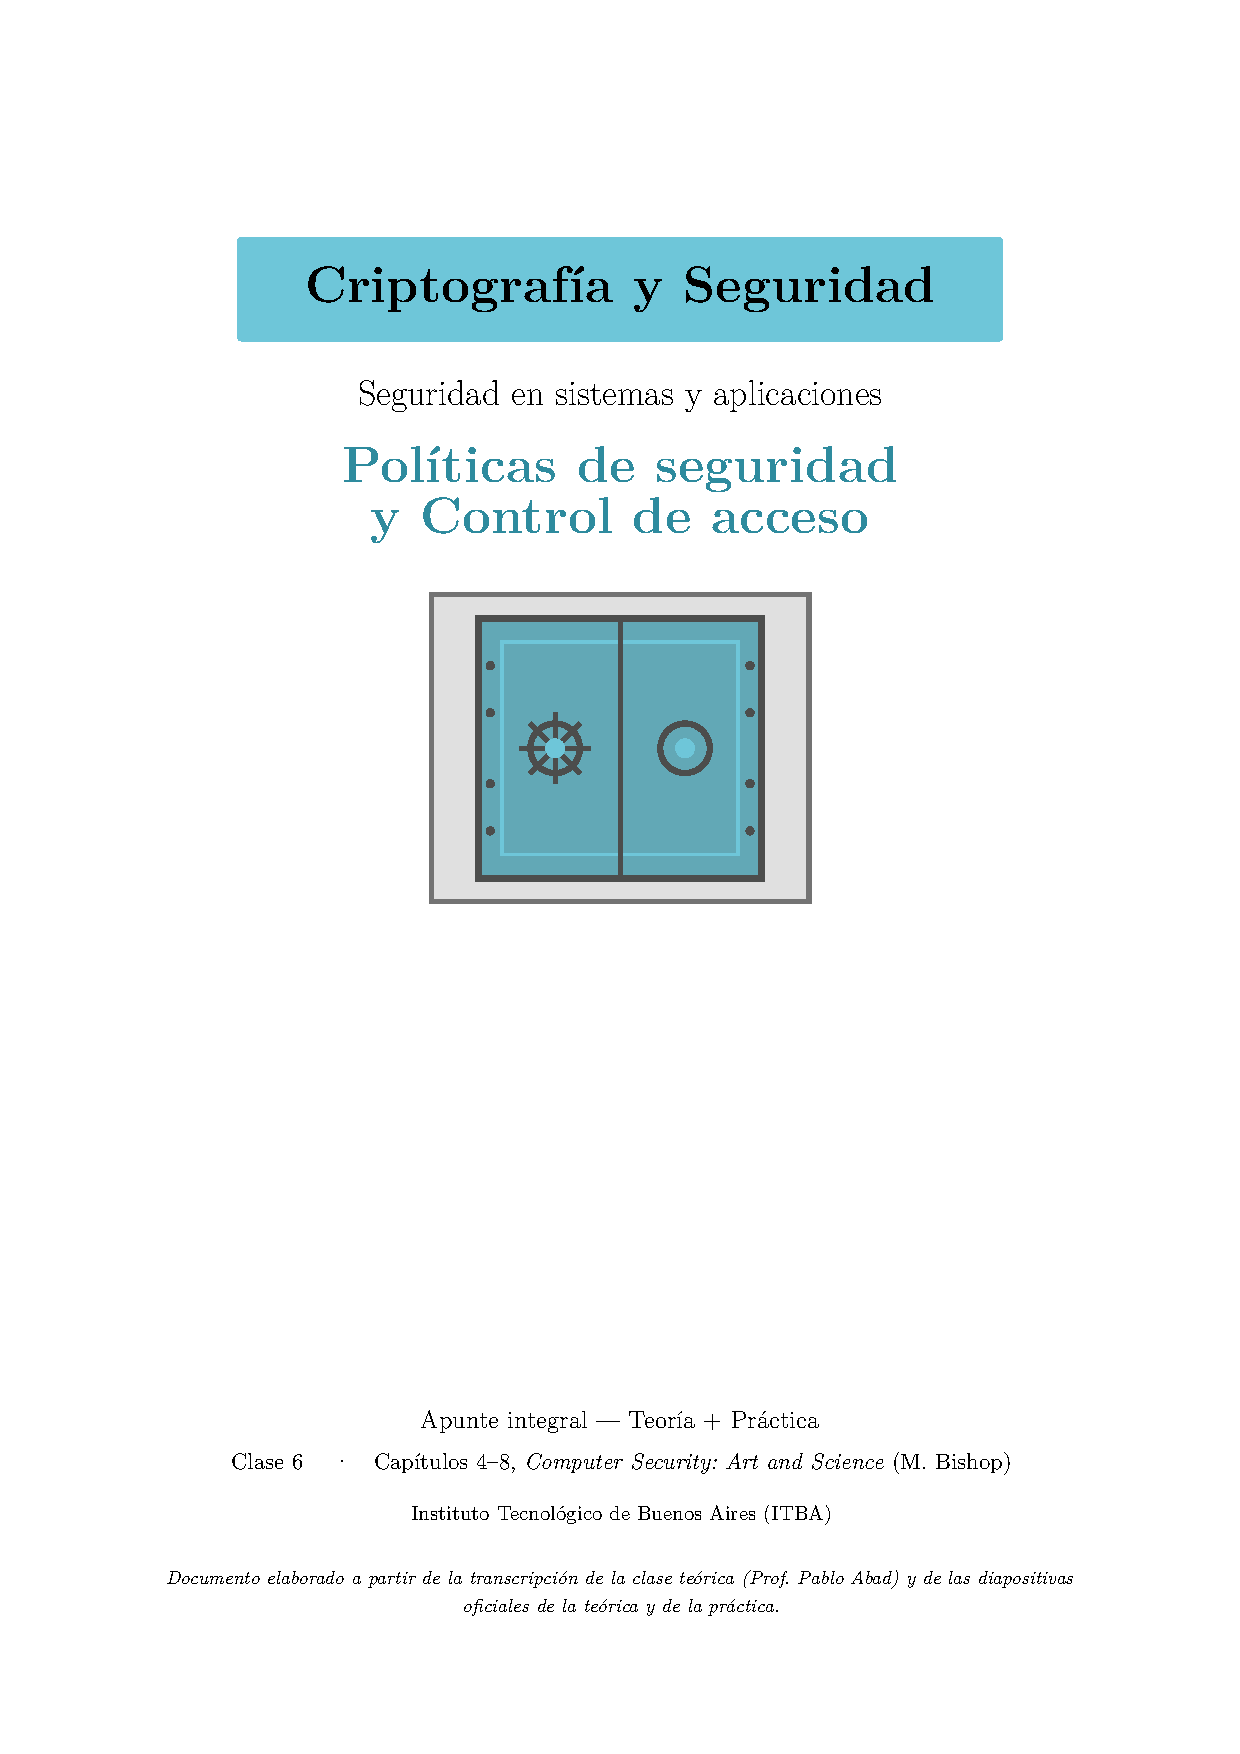
\includepdf[pages=-,addtotoc={1,subsection,2,{Clase 6 — Políticas y Control de Acceso (informe)},toc:c6}]{pdfs/clase06-politicas-control-acceso.pdf}
\phantomsection\label{src:clase7}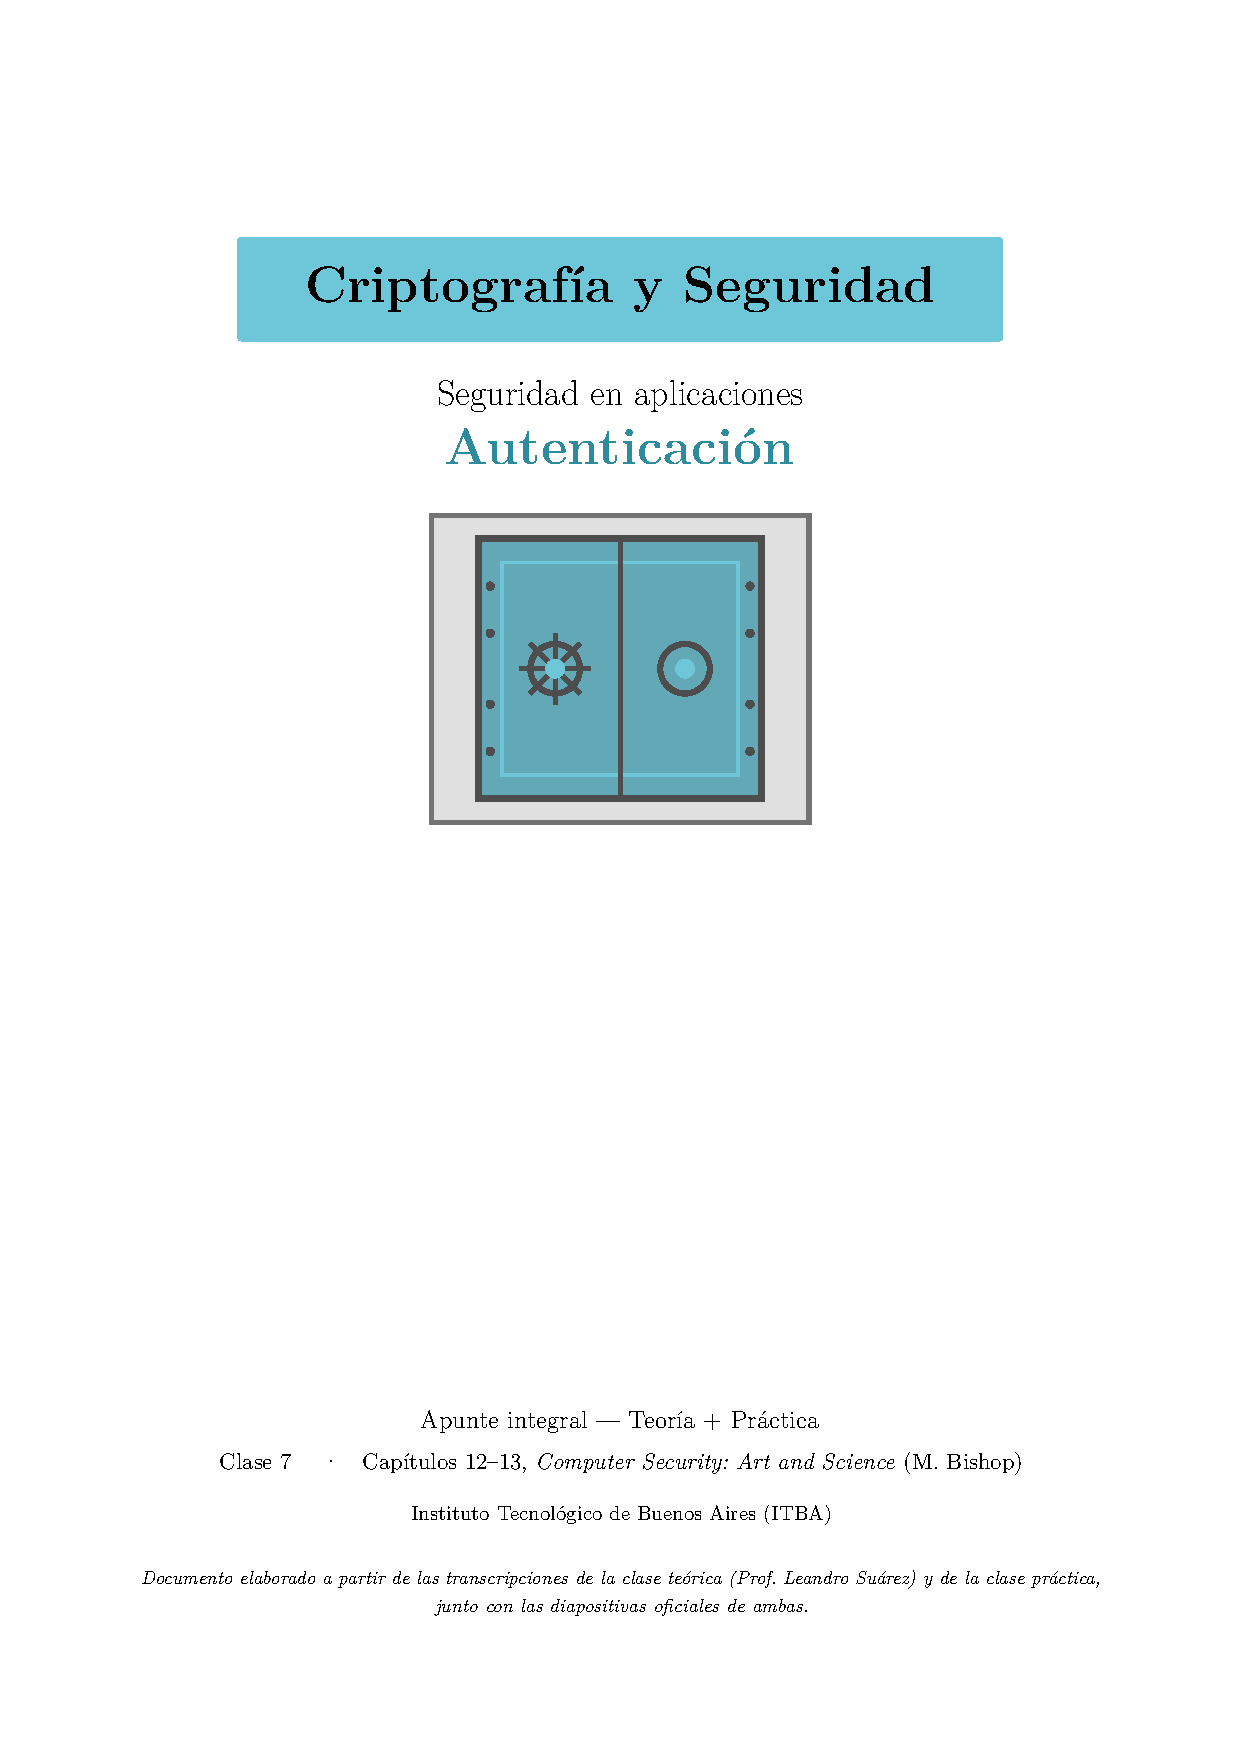
\includepdf[pages=-,addtotoc={1,subsection,2,{Clase 7 — Autenticación (informe)},toc:c7}]{pdfs/clase07-autenticacion.pdf}
\phantomsection\label{src:clase8}
\includepdf[pages=-,addtotoc={1,subsection,2,{Clase 8 — Principios de Diseño y Vulnerabilidades (informe)},toc:c8}]{pdfs/clase08-principios-diseno-seguridad.pdf}
\phantomsection\label{src:clase9}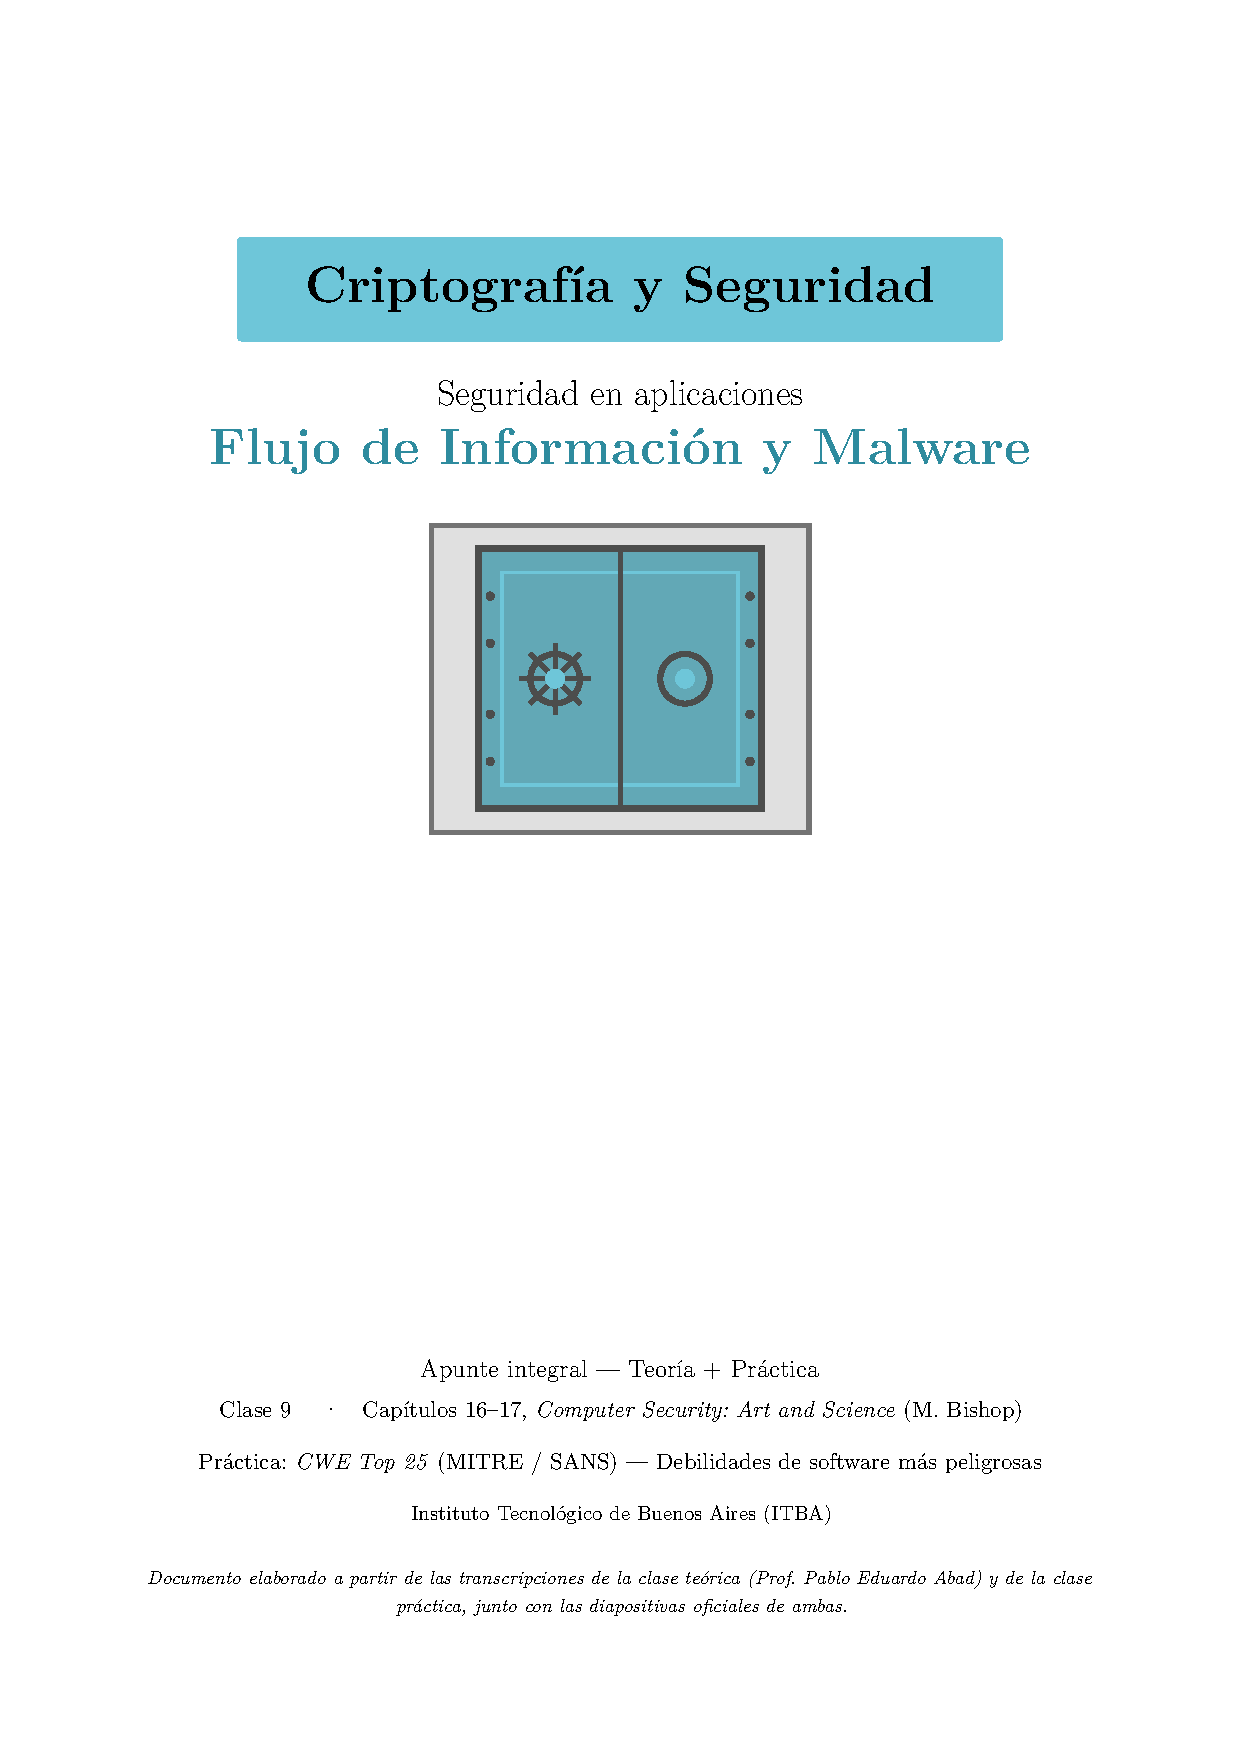
\includepdf[pages=-,addtotoc={1,subsection,2,{Clase 9 — Flujo de Información y Malware (informe)},toc:c9}]{pdfs/clase09-flujo-informacion-malware.pdf}
\phantomsection\label{src:clase10}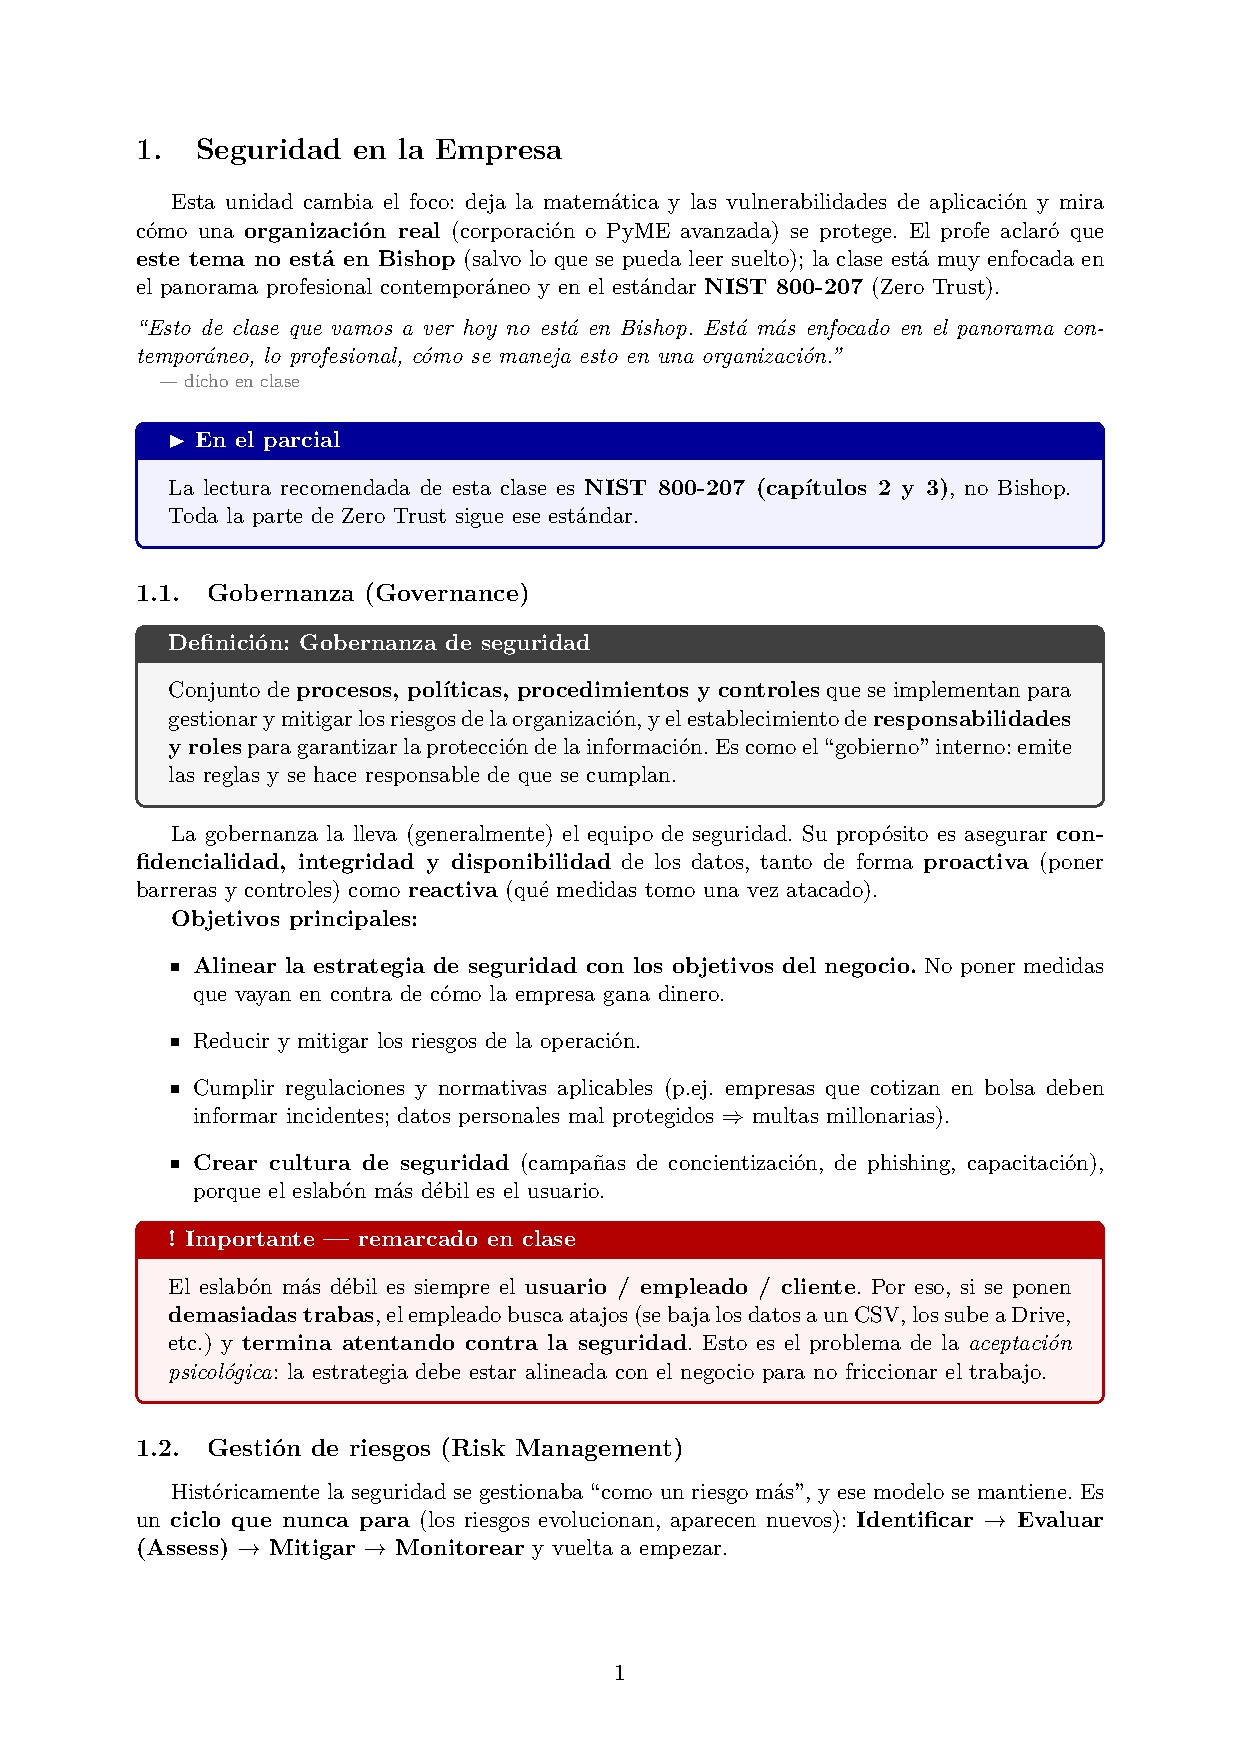
\includepdf[pages=-,addtotoc={1,subsection,2,{Clase 10 — Seguridad en la Empresa (resumen)},toc:c10}]{pdfs/clase10-seguridad-empresa.pdf}
\phantomsection\label{src:clase10b}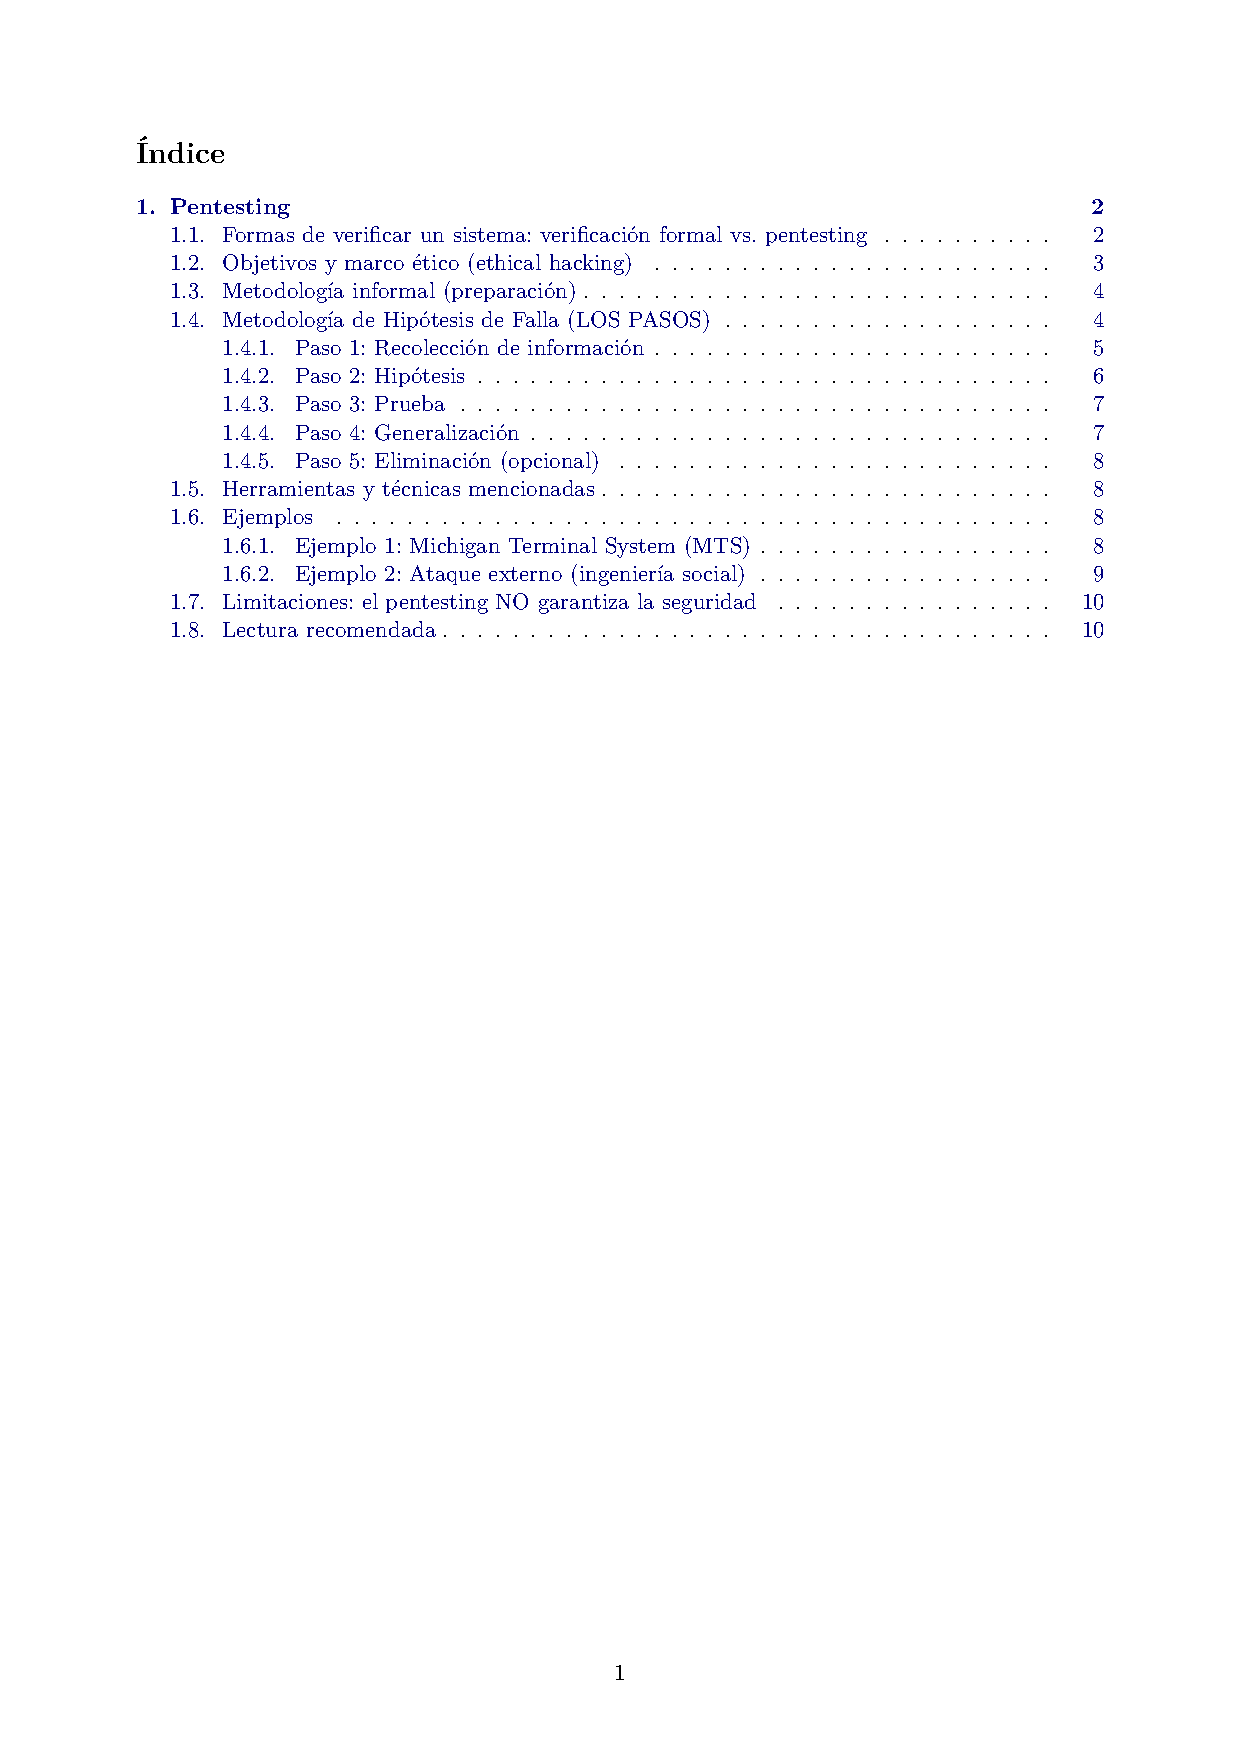
\includepdf[pages=-,addtotoc={1,subsection,2,{Clase 10b — Pentesting (resumen)},toc:c10b}]{pdfs/clase10b-pentesting.pdf}
\phantomsection\label{src:clase11}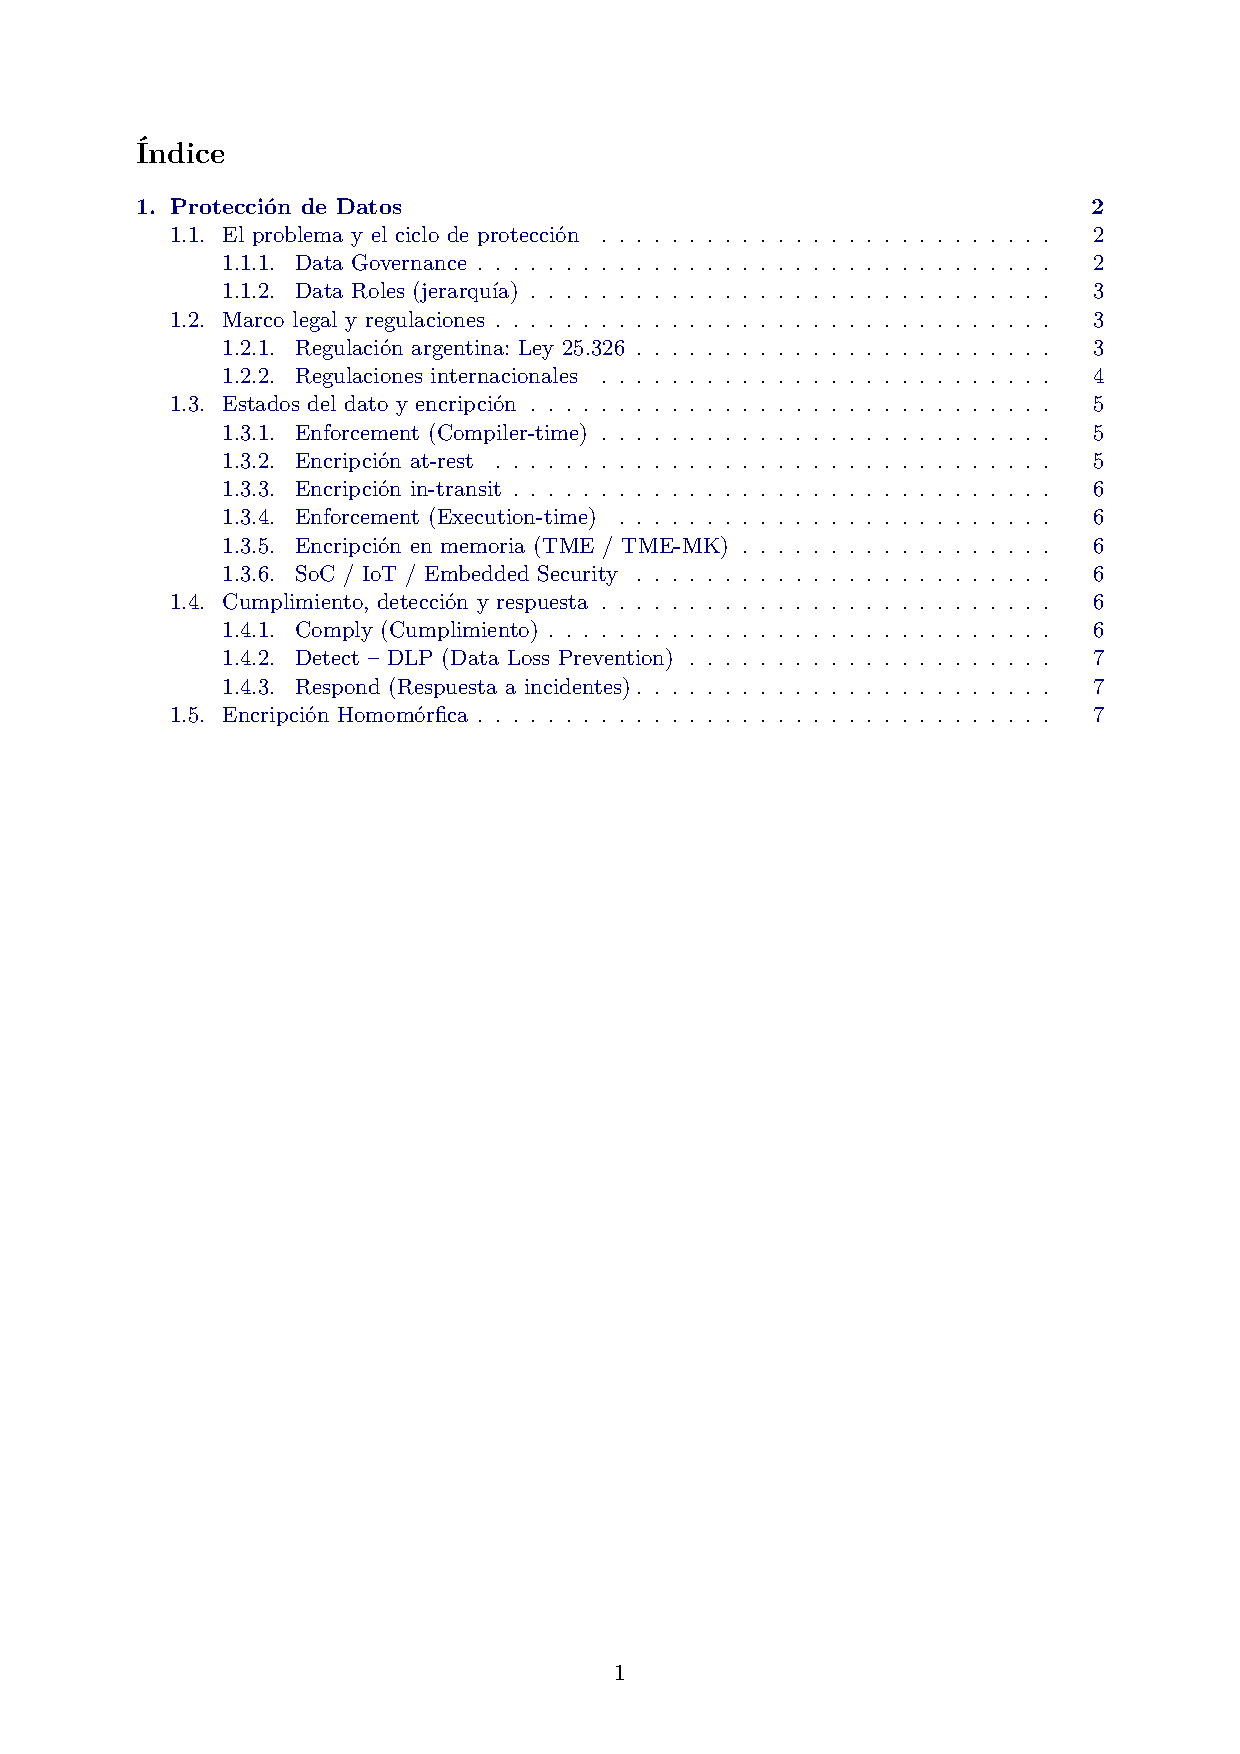
\includepdf[pages=-,addtotoc={1,subsection,2,{Clase 11 — Protección de Datos (resumen)},toc:c11}]{pdfs/clase11-proteccion-datos.pdf}

\phantomsection\label{src:p2013}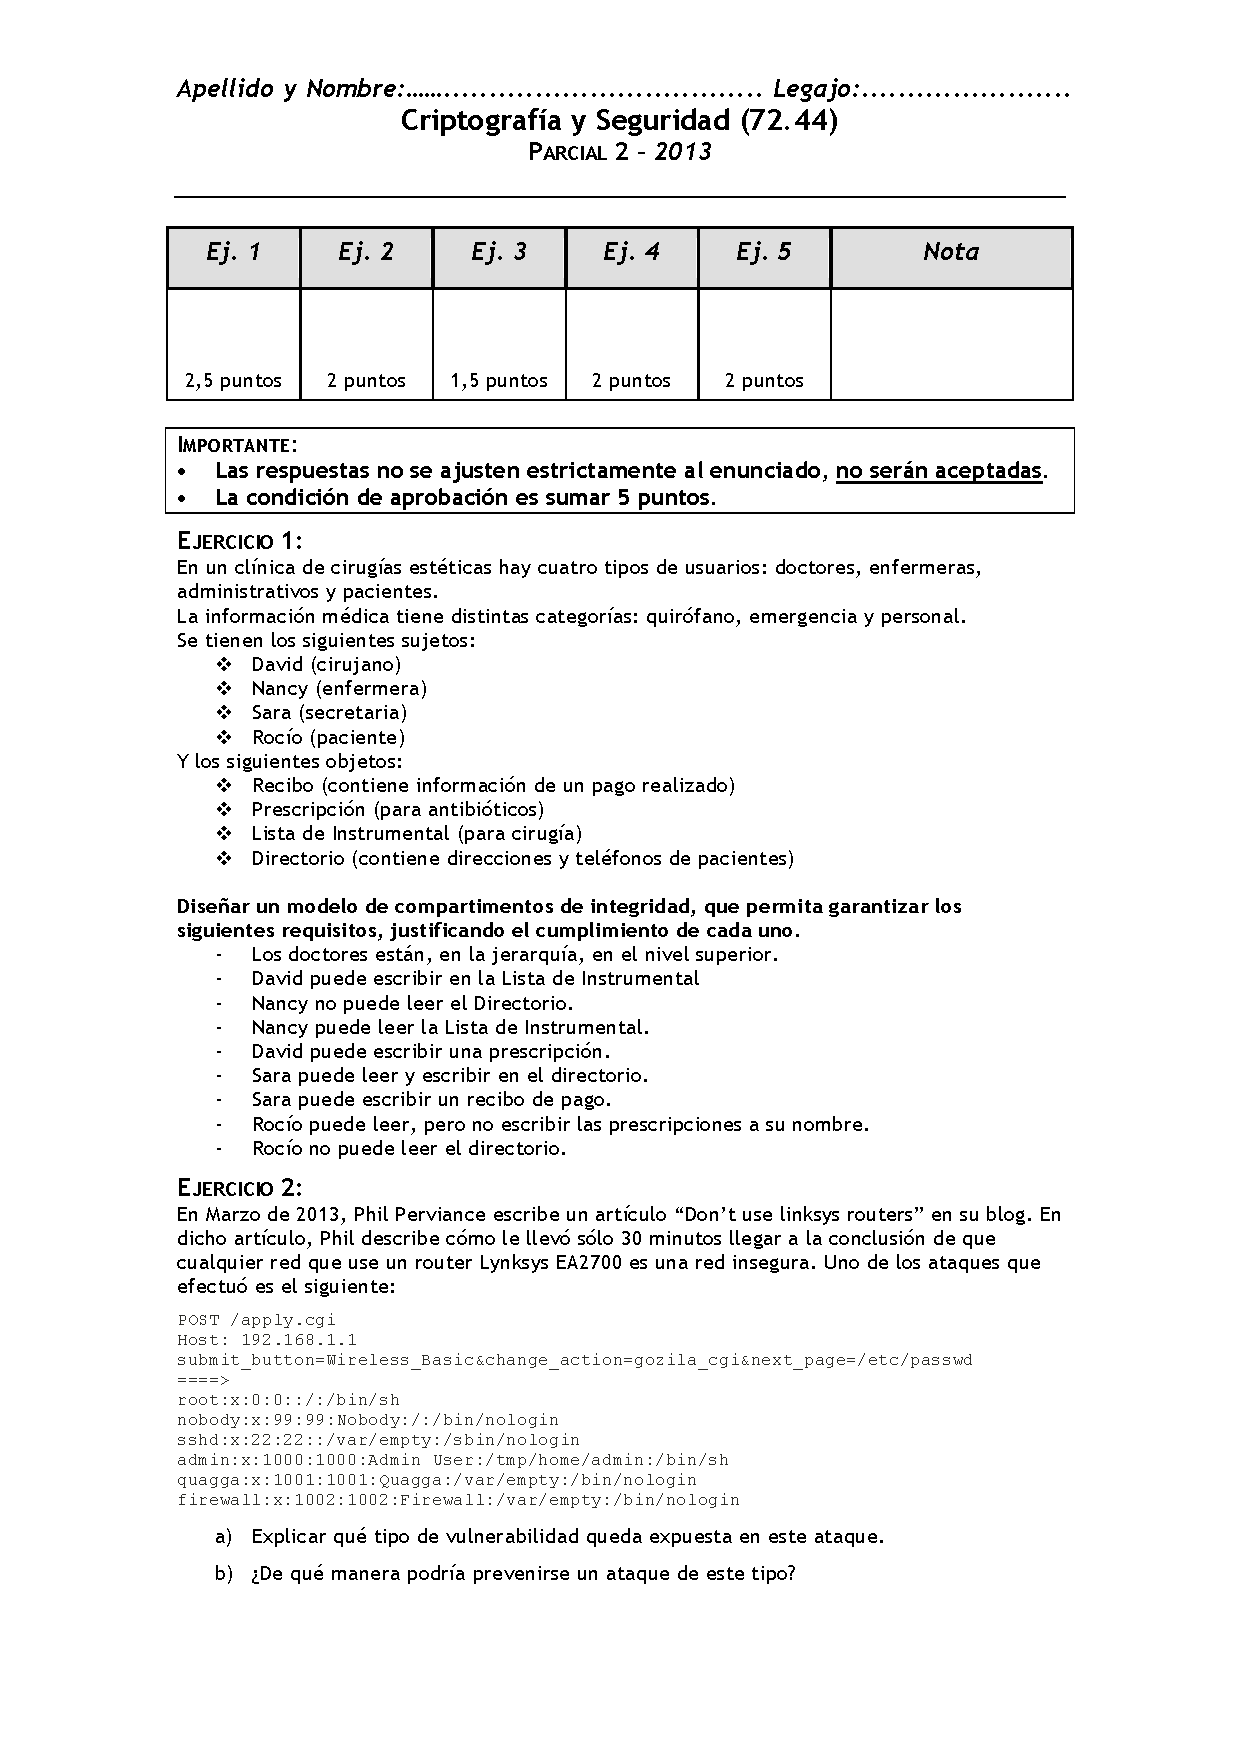
\includepdf[pages=-,addtotoc={1,subsection,2,{Parcial 2013},toc:p2013}]{pdfs/parcial-2013.pdf}
\phantomsection\label{src:p2016}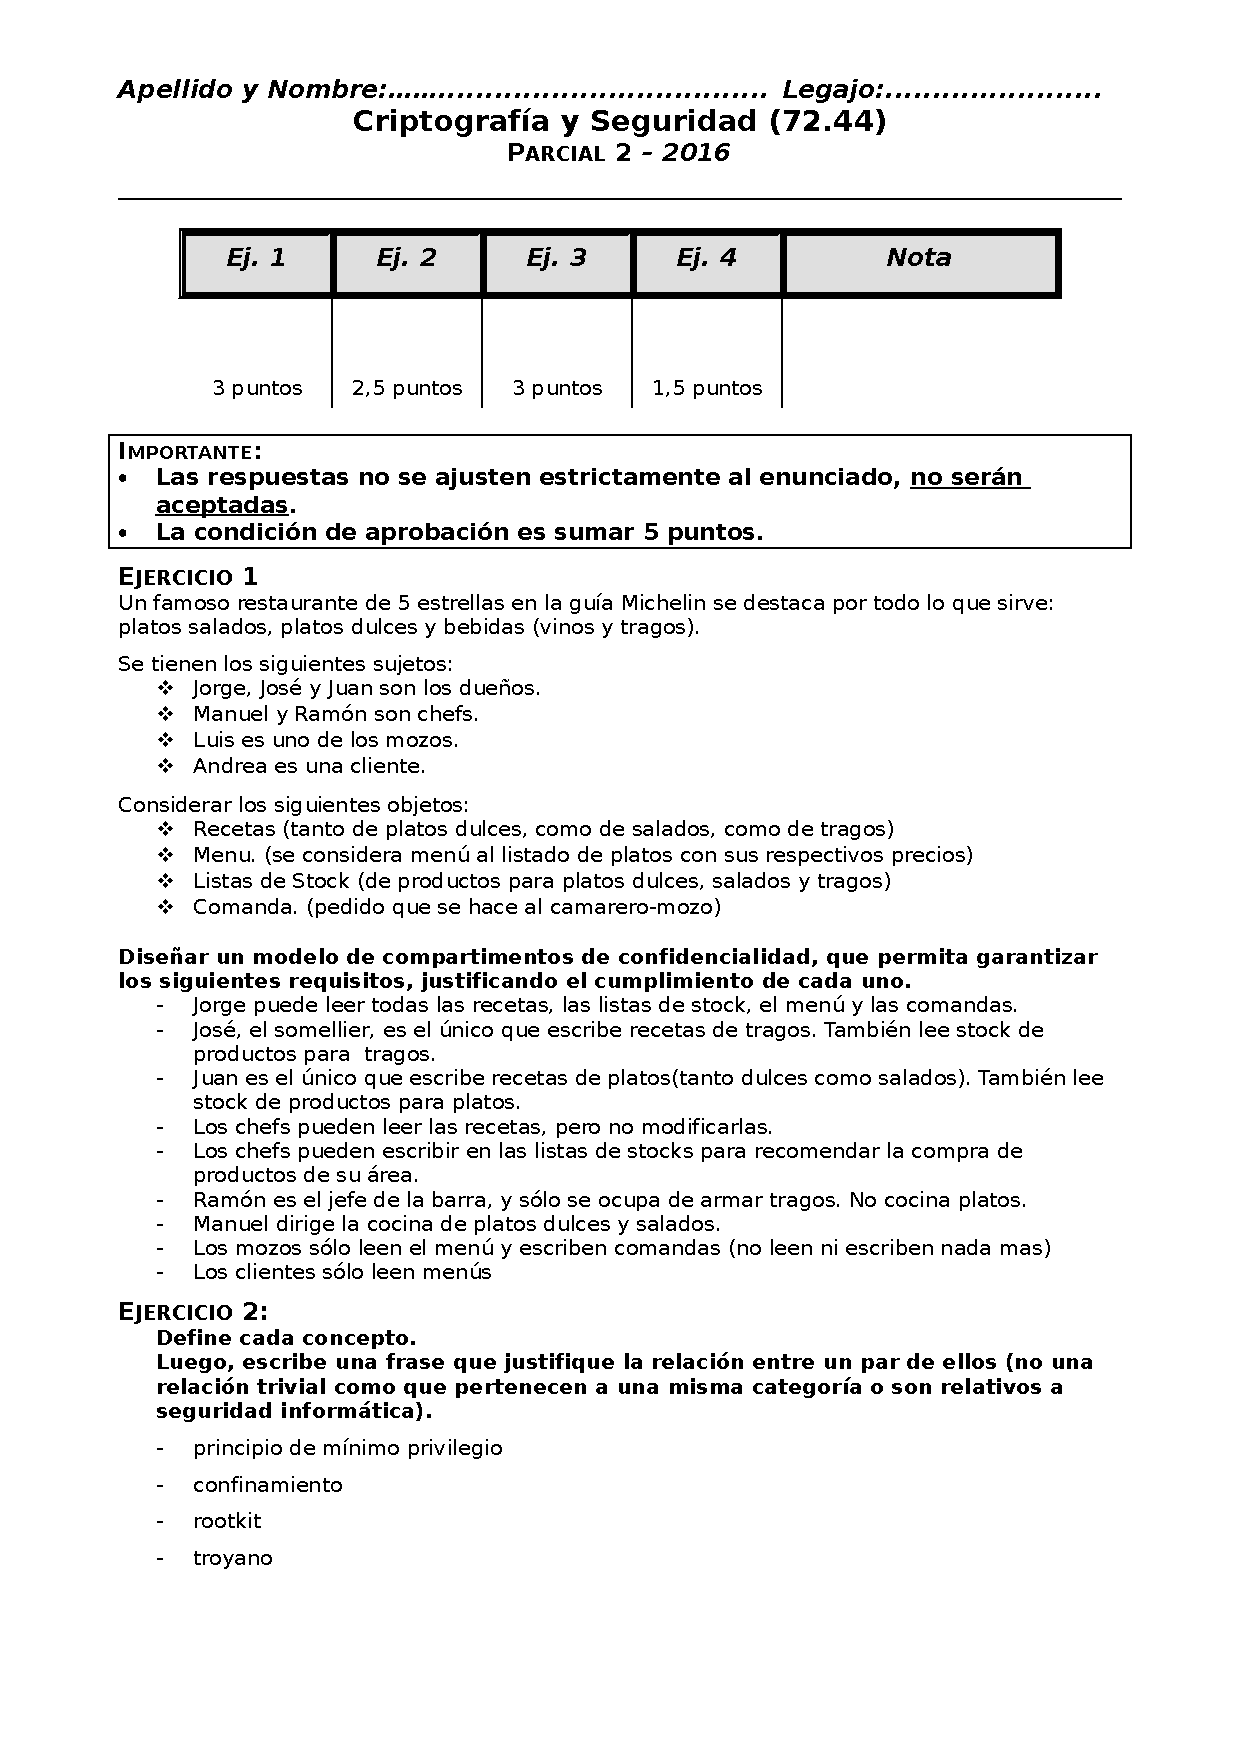
\includepdf[pages=-,addtotoc={1,subsection,2,{Parcial 2016},toc:p2016}]{pdfs/parcial-2016.pdf}
\phantomsection\label{src:p2017}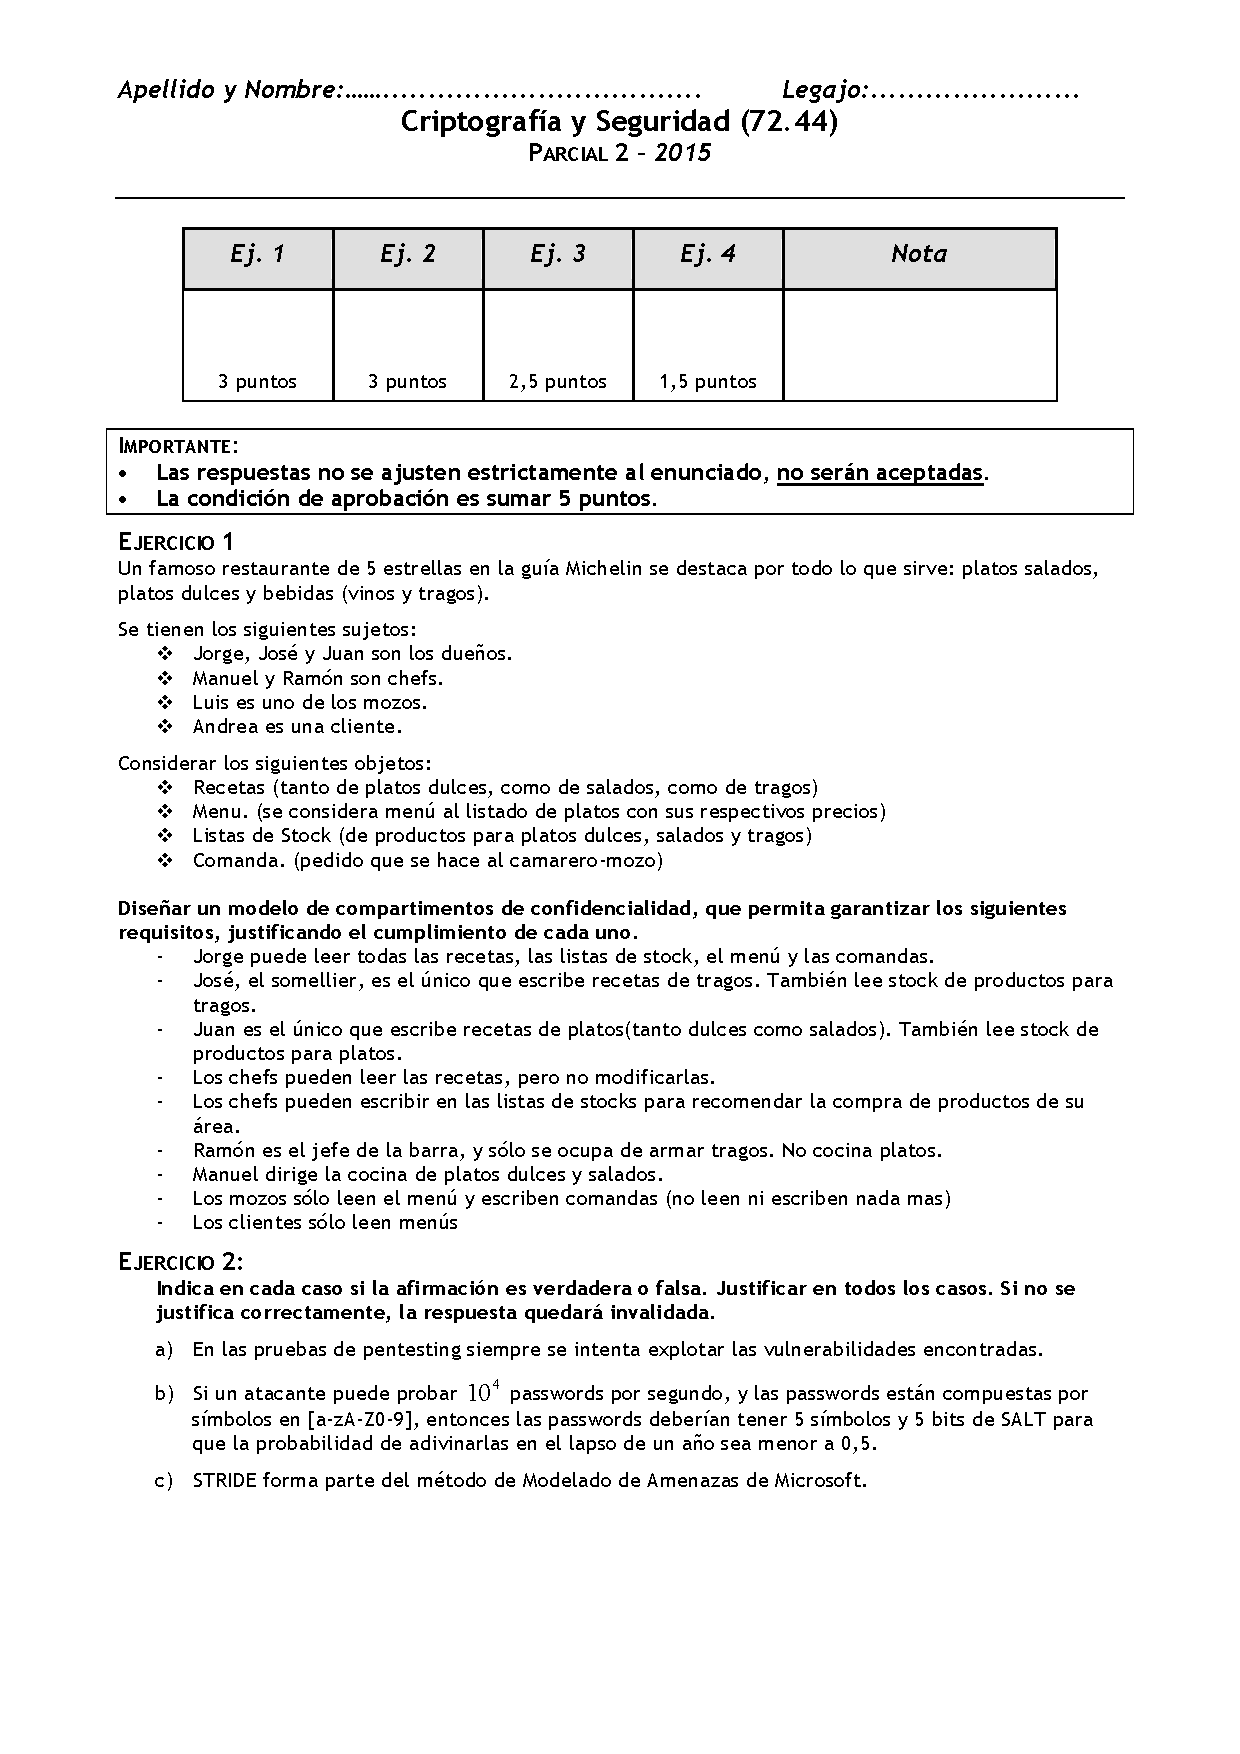
\includepdf[pages=-,addtotoc={1,subsection,2,{Parcial 2017},toc:p2017}]{pdfs/parcial-2017.pdf}
\phantomsection\label{src:p2018}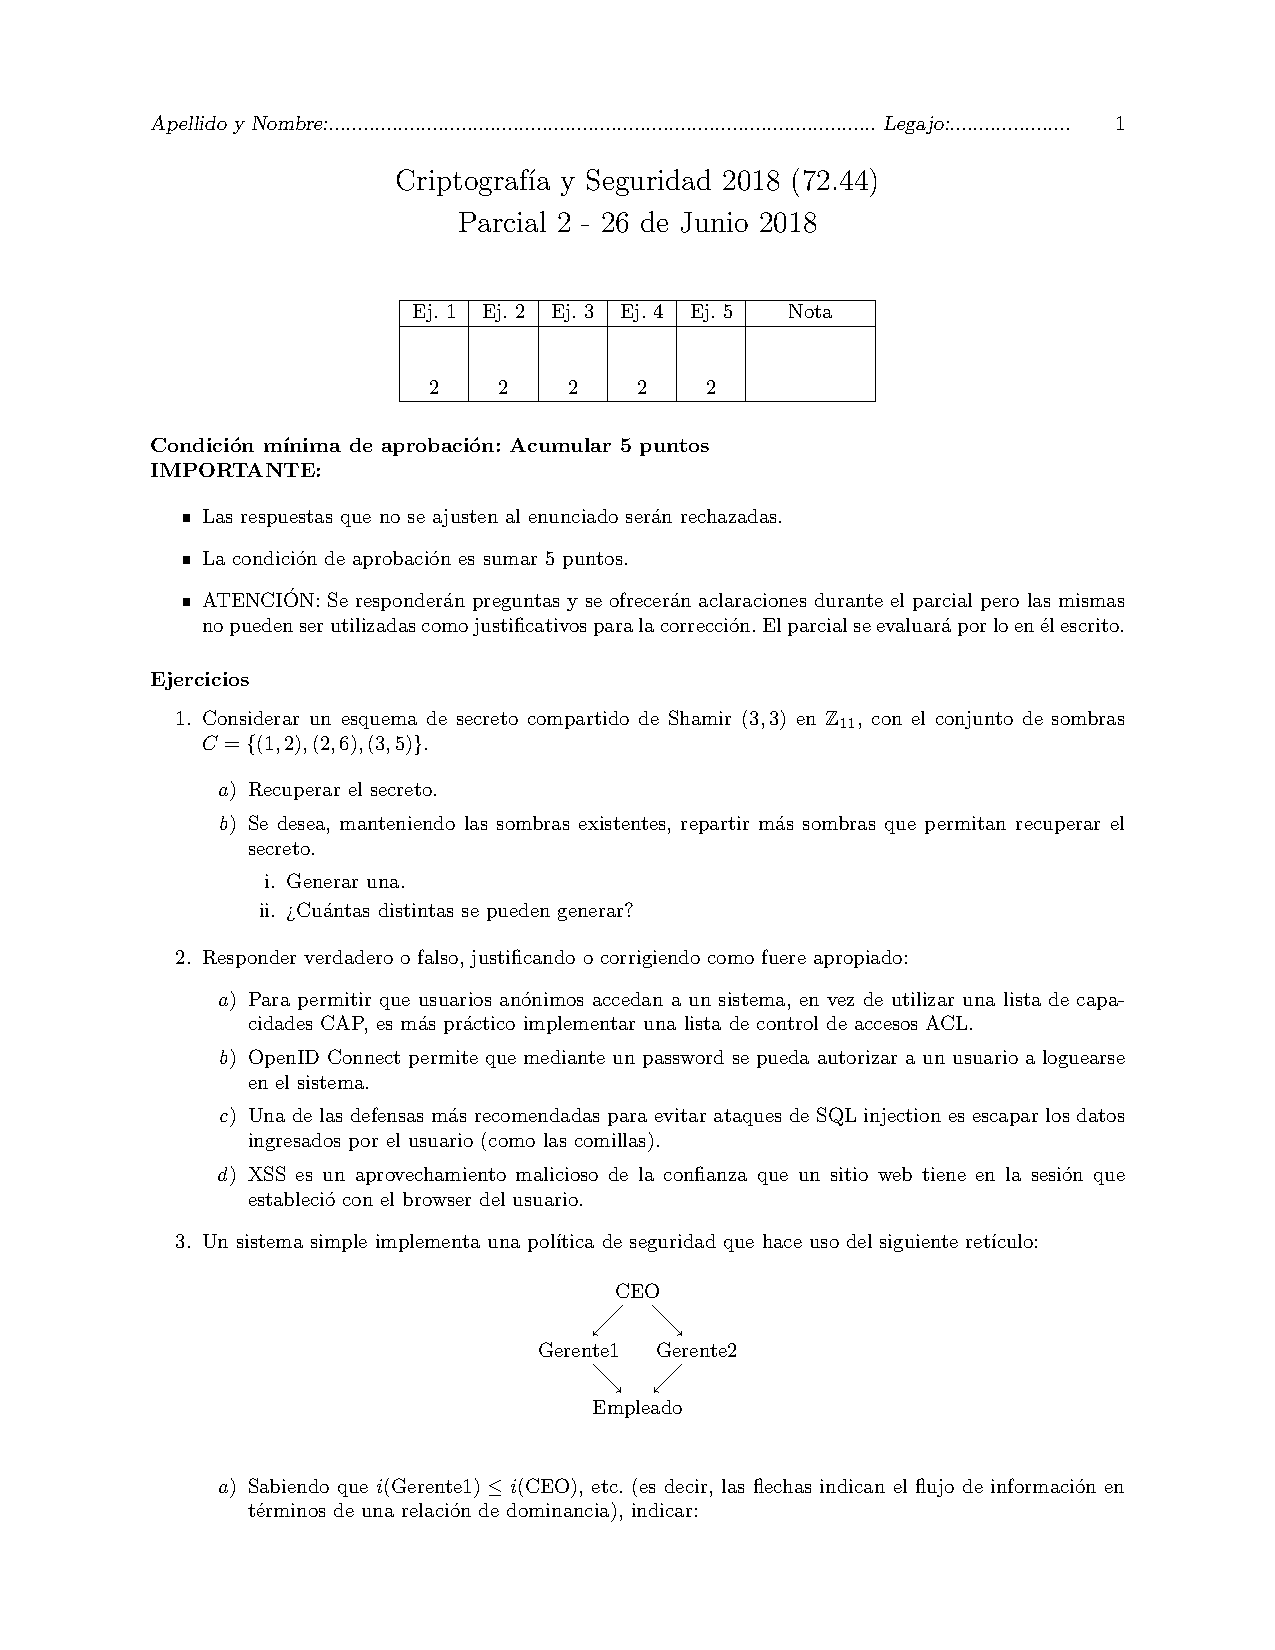
\includepdf[pages=-,addtotoc={1,subsection,2,{Parcial 2018 Q1},toc:p2018}]{pdfs/parcial-2018Q1.pdf}
\phantomsection\label{src:p2023}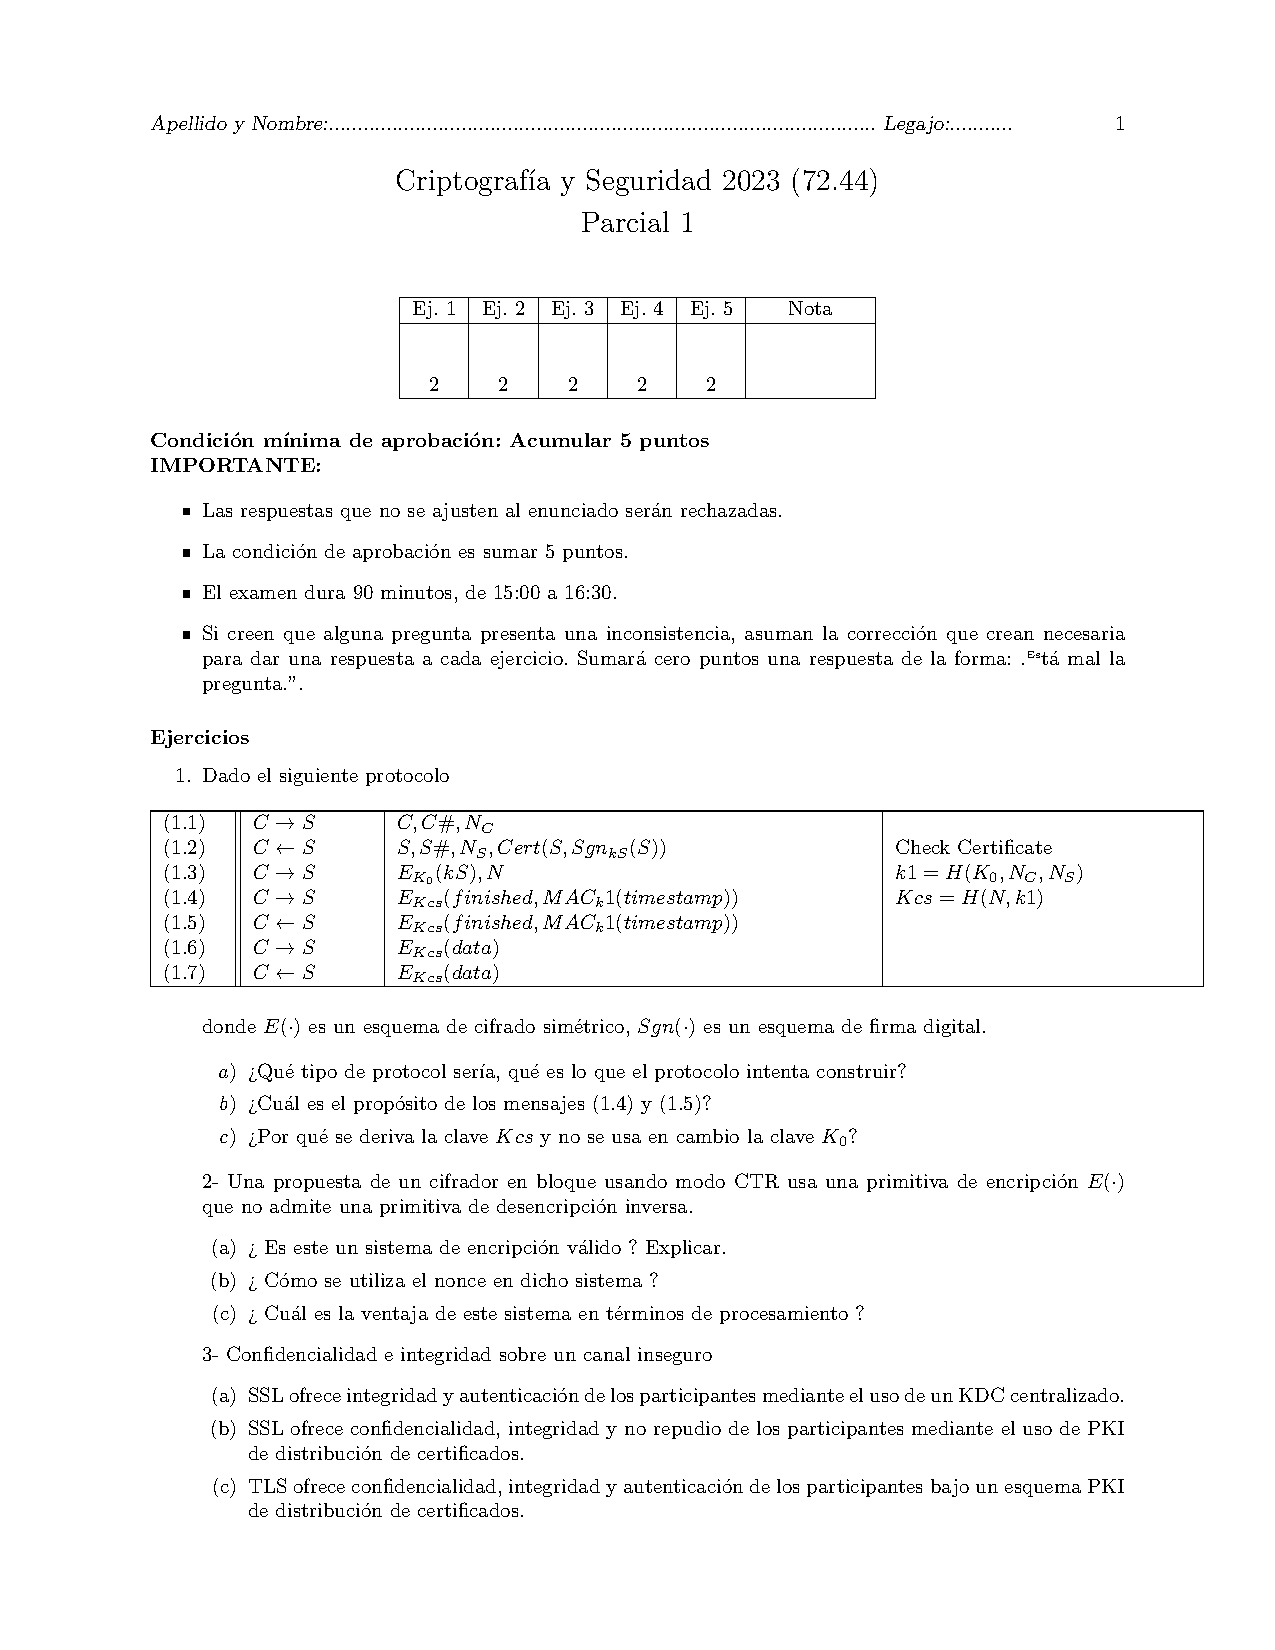
\includepdf[pages=-,addtotoc={1,subsection,2,{Parcial 2023 Q1 (Primera Parte)},toc:p2023}]{pdfs/parcial-2023Q1.pdf}
\phantomsection\label{src:r2023}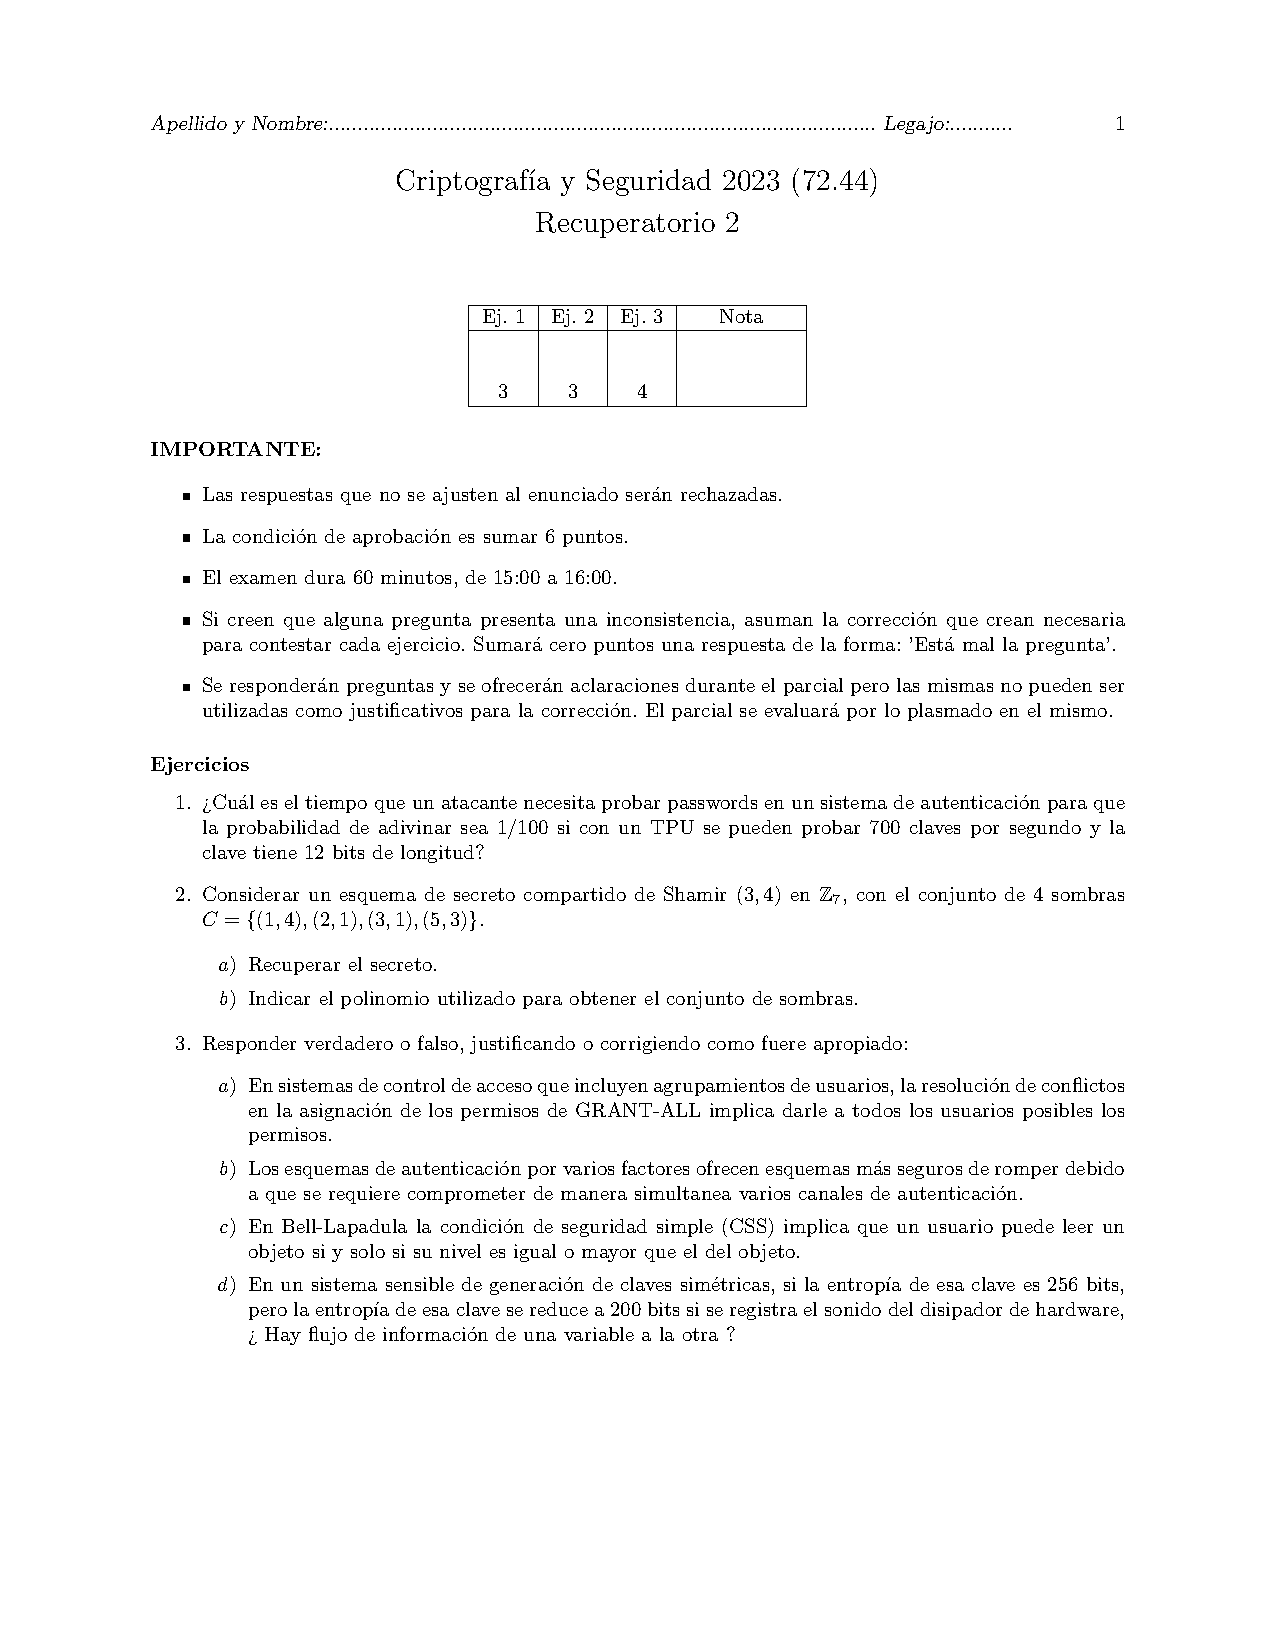
\includepdf[pages=-,addtotoc={1,subsection,2,{Recuperatorio 2023 Q1},toc:r2023}]{pdfs/recup-2023Q1.pdf}
\phantomsection\label{src:p2025q1}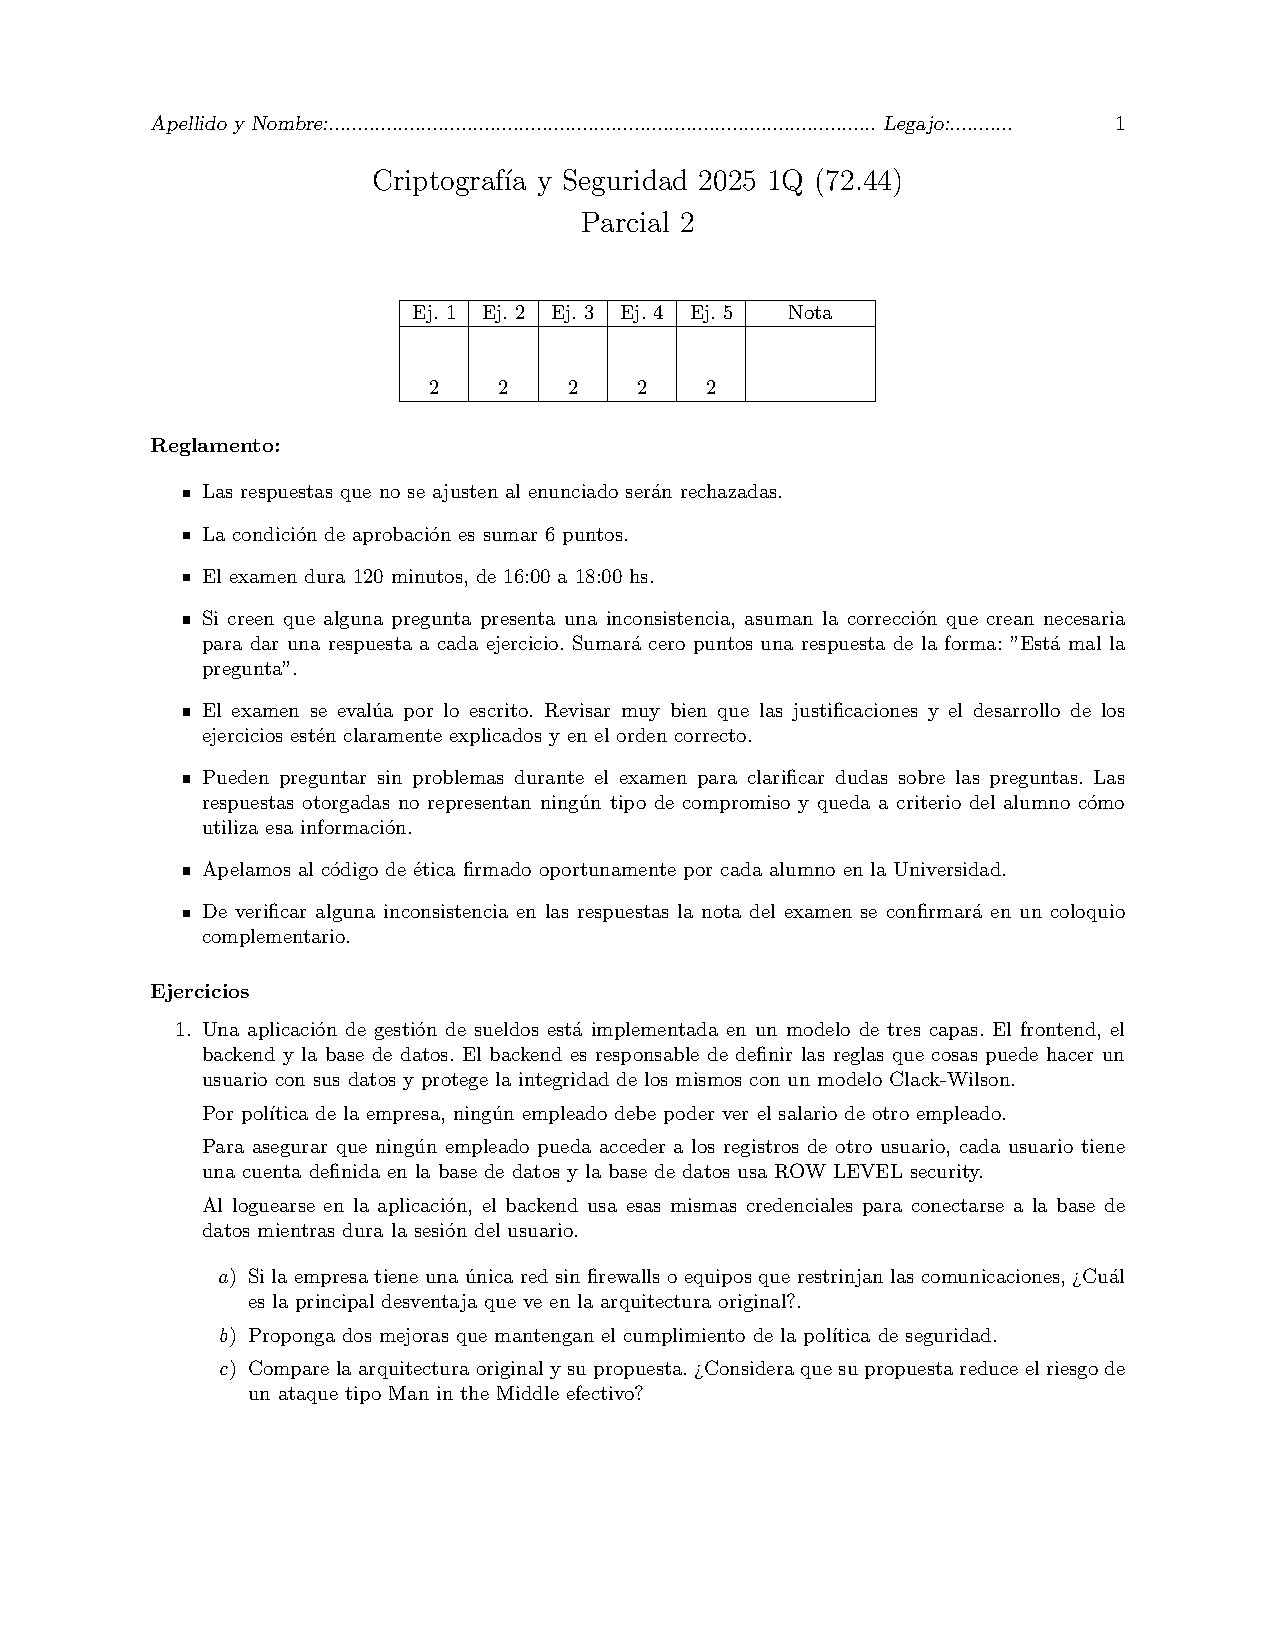
\includepdf[pages=-,addtotoc={1,subsection,2,{Parcial 2025 Q1},toc:p2025q1}]{pdfs/parcial-2025Q1.pdf}
\phantomsection\label{src:r2025q1}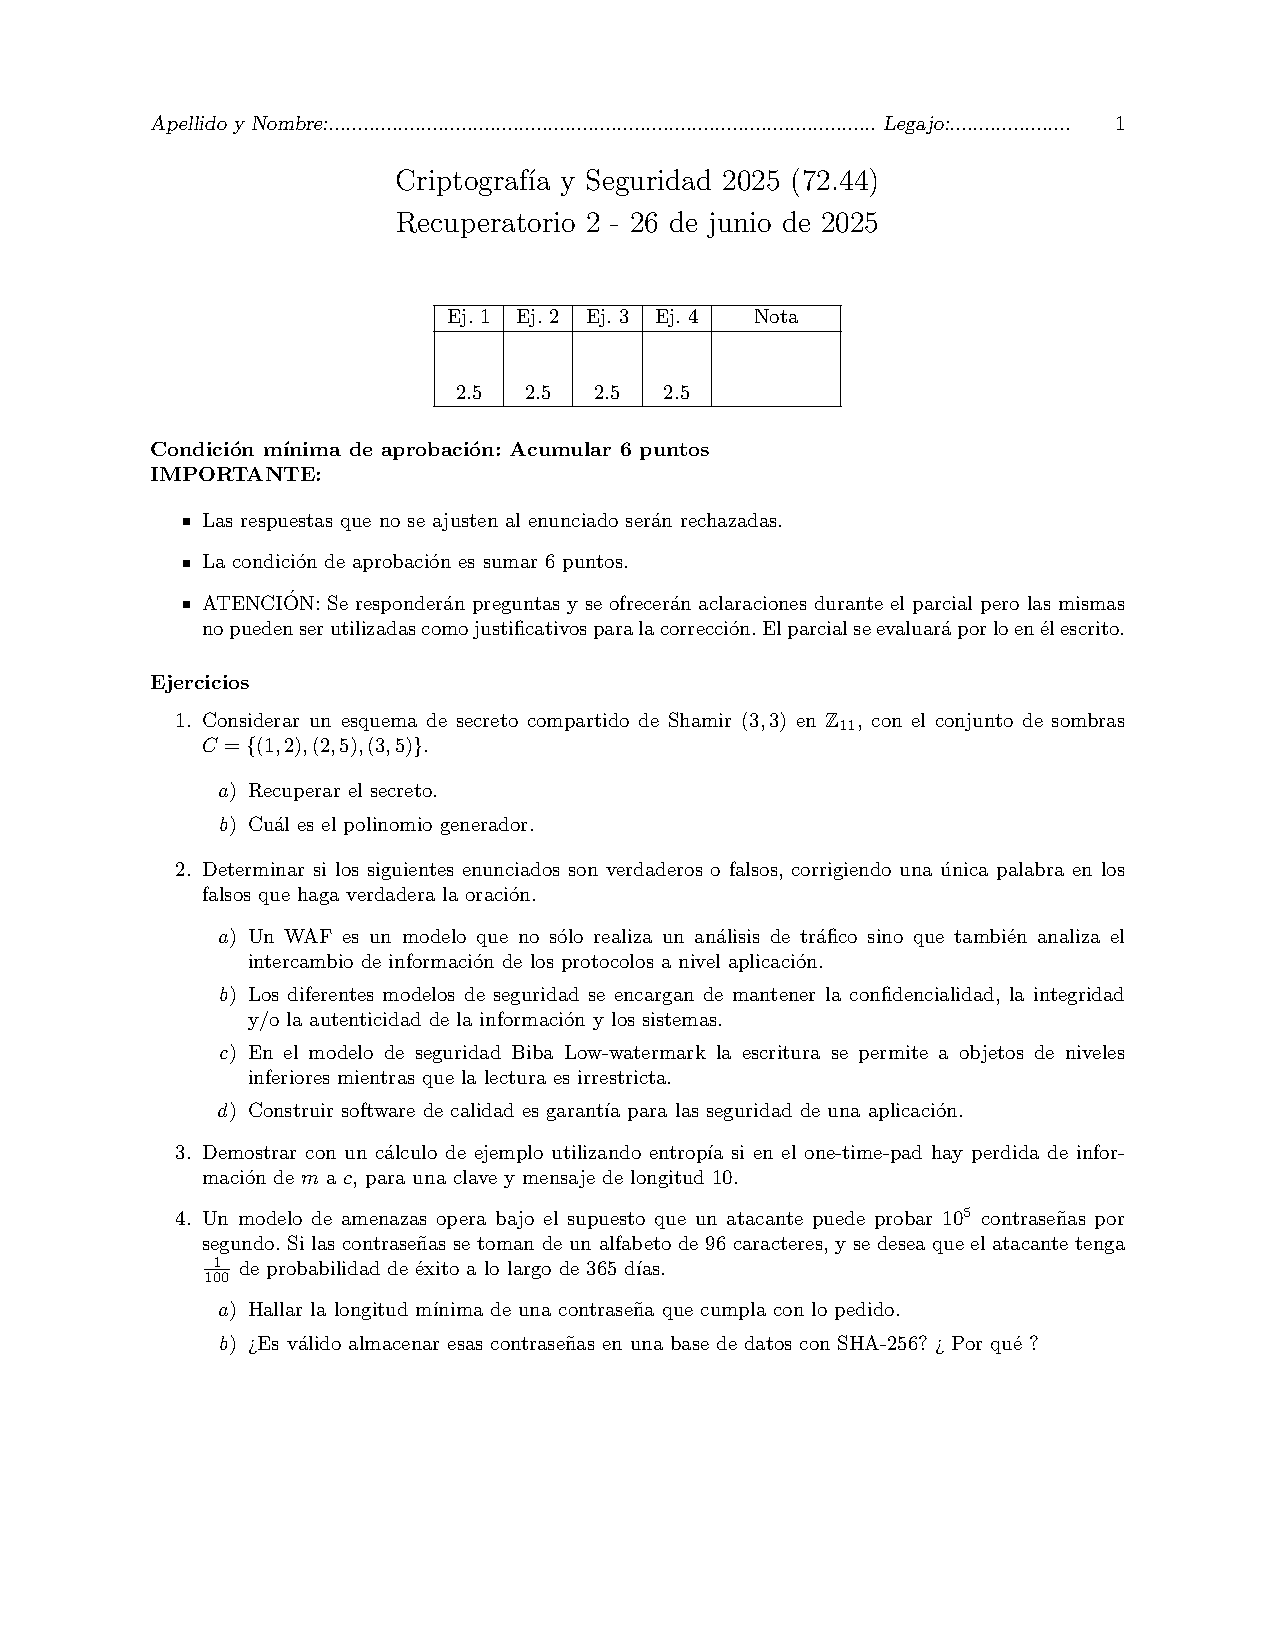
\includepdf[pages=-,addtotoc={1,subsection,2,{Recuperatorio 2025 Q1},toc:r2025q1}]{pdfs/recup-2025Q1.pdf}
\phantomsection\label{src:p2025q2}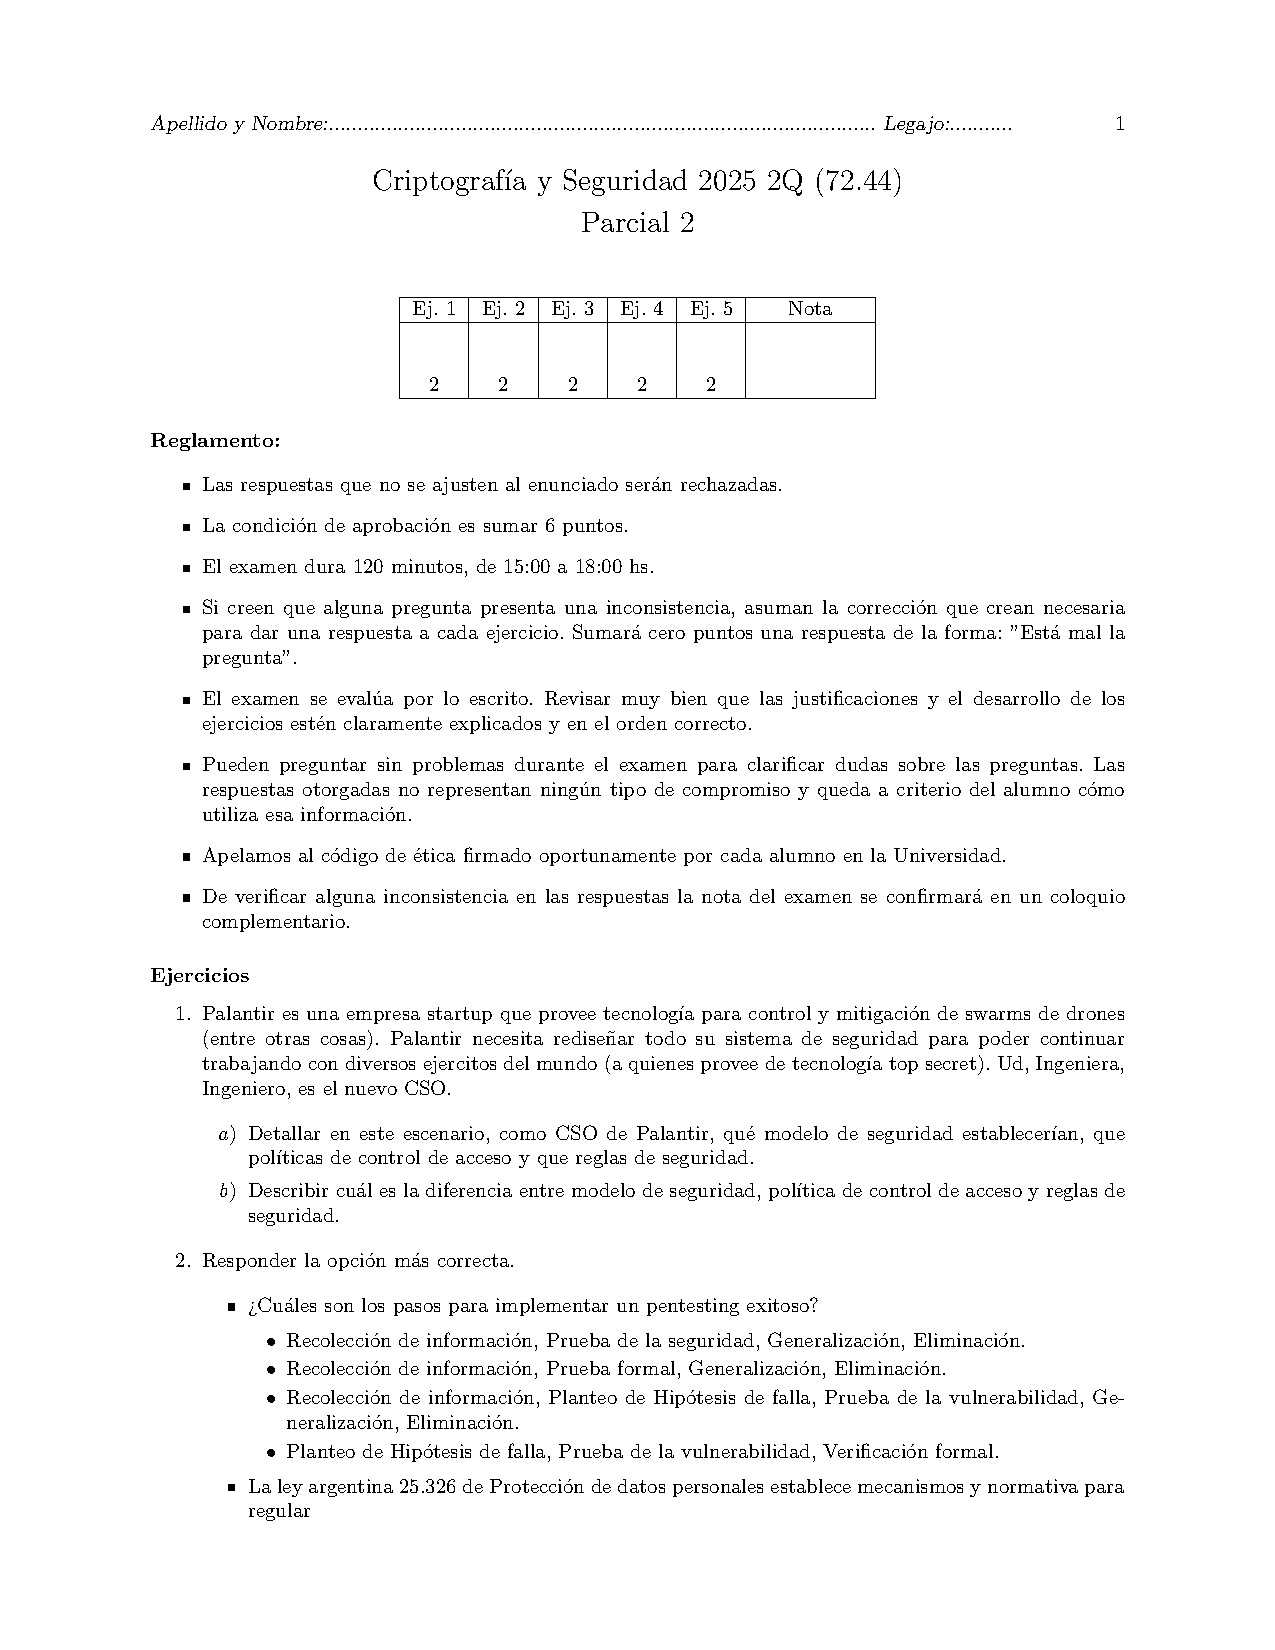
\includepdf[pages=-,addtotoc={1,subsection,2,{Parcial 2025 Q2},toc:p2025q2}]{pdfs/parcial-2025Q2.pdf}

\end{document}
